\documentclass{article}
\usepackage{amsmath}

% Add search paths for input files
\makeatletter
\def\input@path{{../}{../../}{../texinputs/}}
\makeatother

%%
%% Default settings for artisynth
%%
\NeedsTeXFormat{LaTeX2e}
%%\ProvidesPackage{artisynthDoc}[2012/04/05]

\usepackage[T1]{fontenc}
\usepackage[latin1]{inputenc}
\usepackage{listings}
\usepackage{makeidx}
\usepackage{latexml}
\usepackage{graphicx}
\usepackage{framed}
\usepackage{booktabs}
\usepackage{color}

\newcommand{\pubdate}{\today}
\newcommand{\setpubdate}[1]{\renewcommand{\pubdate}{#1}}
\newcommand{\code}[1]{{\tt #1}}

\iflatexml
\usepackage{hyperref}
\setlength\parindent{0pt} 
\else
%% then we are making a PDF, so include things that LaTeXML can't handle: 
%% docbook style, \RaggedRight
\usepackage{ifxetex}
\usepackage{xstring}
\usepackage{pslatex} % fixes fonts; in particular sets a better-fitting \tt font

\usepackage[most]{tcolorbox}
\definecolor{shadecolor}{rgb}{0.95,0.95,0.95}
\tcbset{
    frame code={}
    center title,
    left=0pt,
    right=0pt,
    top=0pt,
    bottom=0pt,
    colback=shadecolor,
    colframe=white,
    width=\dimexpr\textwidth\relax,
    enlarge left by=0mm,
    boxsep=0pt,
    arc=0pt,outer arc=0pt,
}%

\usepackage[A4]{artisynth_papersize}
%\usepackage[letter]{artisynth_papersize}
\usepackage[hyperlink]{asciidoc-dblatex} 

%\usepackage{verbatim}
\usepackage{ragged2e}
\setlength{\RaggedRightRightskip}{0pt plus 4em}
\RaggedRight
\renewcommand{\DBKpubdate}{\pubdate}
\renewcommand{\DBKreleaseinfo}{}
\fi

% set hypertext links to be dark blue:
\definecolor{darkblue}{rgb}{0,0,0.8}
\definecolor{sidebar}{rgb}{0.5,0.5,0.7}
\hypersetup{colorlinks=true,urlcolor=darkblue,linkcolor=darkblue,breaklinks=true}

%%%%%%%%%%%%%%%%%%%%%%%%%%%%%%%%%%%%%%%%%%%%%%%%%%%%%%%%%%%%%%%%%%%%%%%%%%%%%
%
% Define macros for handling javadoc class and method references
%
%%%%%%%%%%%%%%%%%%%%%%%%%%%%%%%%%%%%%%%%%%%%%%%%%%%%%%%%%%%%%%%%%%%%%%%%%%%%%
\makeatletter

% macro to enable line break if inside a PDF file
\def\pdfbreak{\iflatexml\else\\\fi}

% code inspired by http://stackoverflow.com/questions/2457780/latex-apply-an-operation-to-every-character-in-a-string
\def\removeargs #1{\doremoveargs#1$\wholeString\unskip}
\def\doremoveargs#1#2\wholeString{\if#1$%
\else\if#1({()}\else{#1}\taketherest#2\fi\fi}
\def\taketherest#1\fi
{\fi \doremoveargs#1\wholeString}

% Note: still doesn't work properly when called on macro output ...
% i.e., \dottoslash{\concatnames{model}{base}{foo}} fails 
\def\dottoslash #1{\dodottoslash#1$\wholeString\unskip}
\def\dodottoslash#1#2\wholeString{\if#1$%
\else\if#1.{/}\else{#1}\fi\dottaketherest#2\fi}
\def\dottaketherest#1\fi{\fi \dodottoslash#1\wholeString}

\def\hashtodot #1{\dohashtodot#1$\wholeString\unskip}
\def\dohashtodot#1#2\wholeString{\if#1$X%
\else\if#1\#{.}\else{#1}\fi\hashtaketherest#2\fi}
\def\hashtaketherest#1\fi{\fi \dohashtodot#1\wholeString}

%\dollartodot{#1} does the same thing as \StrSubstitute[0]{#1}{\$}{.}
% from the packahe xstring. We define \dollartodot instead because
% LaTeXML does not implement xstring.
%
% Note that for the substituion to work, we need \ifx instead of \if,
% since otherwise escaped characters won't work properly:
% if #1 = \$, then \if#1* seems to compare '\' and '$' (and output '*'),
% rather than comparing '$' to '*'
\def\dollartodot #1{\dodollartodot#1*\wholeString\unskip}
\def\dodollartodot#1#2\wholeString{\ifx#1*%
\else \ifx#1\${.}\else{#1}\fi\dollartaketherest#2\fi}
\def\dollartaketherest#1\fi{\fi \dodollartodot#1\wholeString}

% concatenates up to three class/method names together, adding '.' characters
% between them. The first and/or second argument may be empty, in which case
% the '.' is omitted. To check to see if these arguments are empty, we
% use a contruction '\if#1@@', which will return true iff #1 is empty
% (on the assumption that #1 will not contain a '@' character).
\def\concatnames
#1#2#3{\if#1@@\if#2@@#3\else #2.#3\fi\else\if#2@@#1.#3\else#1.#2.#3\fi\fi}

\newcommand{\javabase}{}
\newcommand{\setjavabase}[1]{\renewcommand{\javabase}{#1}}

\def\artisynthDocBase{@ARTISYNTHDOCBASE}

\iflatexml
\def\ifempty#1{\def\temp{#1}\ifx\temp\empty}%
\newcommand{\artisynthManual}[3][]{%
   \ifempty{#1}
      \href{@ARTISYNTHDOCBASE/#2/#2.html}{#3}%
    \else
      \href{@ARTISYNTHDOCBASE/#1/#2.html}{#3}%
    \fi
}
\else
\newcommand{\artisynthManual}[3][]{%
\href{https://www.artisynth.org/@ARTISYNTHDOCBASE/#2.pdf}{#3}}
\fi

%\href{@ARTISYNTHDOCBASE/#2/#2.html}{#3}}



\newcommand{\javaclassx}[2][]{%
% Includes code to prevent an extra '.' at the front if #1 is empty. It
% works like this: if '#1' is empty, then '#1.' expands to '.', and so 
% '\if#1..' will return true, in which case we just output '#2'.
\href{@JDOCBEGIN/\concatnames{\javabase}{#1}{#2}@JDOCEND}{#2}}
\newcommand{\javaclass}[2][]{%
\href{@JDOCBEGIN/\concatnames{}{#1}{#2}@JDOCEND}{\dollartodot{#2}}}
\newcommand{\javaclassAlt}[2]{%
\href{@JDOCBEGIN/\concatnames{}{}{#1}@JDOCEND}{#2}}

\newcommand{\javamethodArgsx}[2][]{%
\href{@JDOCBEGIN/\concatnames{\javabase}{#1}{#2}@JDOCEND}{#2}}
\newcommand{\javamethodArgs}[2][]{%
\href{@JDOCBEGIN/\concatnames{}{#1}{#2}@JDOCEND}{#2}}
\newcommand{\javamethodAlt}[2]{%
\href{@JDOCBEGIN/\concatnames{}{}{#1}@JDOCEND}{#2}}
\newcommand{\javamethodAltx}[2]{%
\href{@JDOCBEGIN/\concatnames{\javabase}{}{#1}@JDOCEND}{#2}}

\newcommand{\javamethodNoArgsx}[2][]{%
\href{@JDOCBEGIN/\concatnames{\javabase}{#1}{#2}@JDOCEND}{\removeargs{#2}}}
\newcommand{\javamethodNoArgs}[2][]{%
\href{@JDOCBEGIN/\concatnames{}{#1}{#2}@JDOCEND}{\removeargs{#2}}}

\newcommand{\javamethod}{\@ifstar\javamethodNoArgs\javamethodArgs}
\newcommand{\javamethodx}{\@ifstar\javamethodNoArgsx\javamethodArgsx}

%%%%%%%%%%%%%%%%%%%%%%%%%%%%%%%%%%%%%%%%%%%%%%%%%%%%%%%%%%%%%%%%%%%%%%%%%%%%%
%
% Define macros for sidebars
%
%%%%%%%%%%%%%%%%%%%%%%%%%%%%%%%%%%%%%%%%%%%%%%%%%%%%%%%%%%%%%%%%%%%%%%%%%%%%%

\iflatexml
\newenvironment{sideblock}{\begin{quote}}{\end{quote}}
\else
\usepackage[strict]{changepage}
\definecolor{sidebarshade}{rgb}{1.0,0.97,0.8}
\newenvironment{sideblock}{%
    \def\FrameCommand{%
    \hspace{1pt}%
    {\color{sidebar}\vrule width 2pt}%
    %{\vrule width 2pt}%
    {\color{sidebarshade}\vrule width 4pt}%
    \colorbox{sidebarshade}%
  }%
  \MakeFramed{\advance\hsize-\width\FrameRestore}%
  \noindent\hspace{-4.55pt}% disable indenting first paragraph
  \begin{adjustwidth}{}{7pt}%
  %\vspace{2pt}\vspace{2pt}%
}
{%
  \vspace{2pt}\end{adjustwidth}\endMakeFramed%
}
\fi

\iflatexml
\newenvironment{shadedregion}{%
  \definecolor{shadecolor}{rgb}{0.96,0.96,0.98}%
  \begin{shaded*}%
% Put text inside a quote to create a surrounding blockquote that
% will properly accept the color and padding attributes
  \begin{quote}%
}
{%
  \end{quote}%
  \end{shaded*}%
}
\else
\newenvironment{shadedregion}{%
  \definecolor{shadecolor}{rgb}{0.96,0.96,0.98}%
  \begin{shaded*}%
}
{%
  \end{shaded*}%
}
\fi

% Wanted to create a 'listing' environment because lstlisting is
% tedious to type and because under latexml it may need
% some massaging to get it to work properly. But hard to do
% because of the verbatim nature of listing
%\iflatexml
%\newenvironment{listing}{\begin{lstlisting}}{\end{lstlisting}}%
%\else
%\newenvironment{listing}{\begin{lstlisting}}{\end{lstlisting}}%
%\fi

\iflatexml\else
% fancyhdr was complaining that it wanted a 36pt header height ...
\setlength{\headheight}{36pt}
\fi

% macro for backslash character
\newcommand\BKS{\textbackslash}

% macro for double hyphen (to prevent conversion of -- into -)
\newcommand\DHY{-{}-}

% Convenience stuff
\newcommand{\ifLaTeXMLelse}[2]{%
  \iflatexml %
  #1 %
  \else %
  #2 %
  \fi %
}

\newcommand{\ifLaTeXML}[1]{ %
  \iflatexml %
  #1 %
  \fi %
}

% new methodtable environment for documenting methods

% base width of the method table
\newlength{\methodtablewidth}
\iflatexml
\setlength{\methodtablewidth}{1.4\textwidth}
\else
\setlength{\methodtablewidth}{0.94\textwidth}
\fi
% horizontal space added at end of call to \methodentry
\newlength{\methodskip}
\setlength{\methodskip}{0pt}
% lengths set inside methodtable environment:
\newlength{\methodsiglength} % length of the method signature
\newlength{\methodcomlength} % length of the method comment
\setlength{\methodsiglength}{0.5\methodtablewidth}
\setlength{\methodcomlength}{0.5\methodtablewidth}

% command to add a method to a method table:
% arg #1: package and signature for finding URL
% arg #2: anchor text
% arg #3: comment describing the method
\newcommand{\methodentry}[3]{%
\javamethodAlt{#1}{\parbox[t]{\methodsiglength}{#2}}&
{\parbox[t]{\methodcomlength}{#3}}\\%
\noalign{\vspace{\methodskip}}}

% methodtable environment takes two arguments, both scale factors for
% methodtablewidth:
% arg #1: width of the method signature column
% arg #2: width of the method comment column
\newenvironment{methodtable}[3][0pt]{%
\begingroup
\setlength{\topskip}{0pt}
\setlength{\methodskip}{#1}
\setlength{\methodsiglength}{#2\methodtablewidth}%
\setlength{\methodcomlength}{#3\methodtablewidth}%
\iflatexml
\begin{snugshade}
\else
\begin{tcolorbox}
\fi
\renewcommand{\arraystretch}{1}
\begin{tabular}{ll}}{%
\end{tabular}
\renewcommand{\arraystretch}{1}
\iflatexml
\end{snugshade}
\else
\end{tcolorbox}
\fi
\endgroup}

% commands for added top, mid and bottom lines in the table.
% uses booktabs for PDF, regular hline for HTML
\newcommand{\topline}{\iflatexml\hline\else\toprule\fi}
\newcommand{\midline}{\iflatexml\hline\else\midrule\fi}
\newcommand{\botline}{\iflatexml\hline\else\bottomrule\fi}
\newcommand{\blankline}{%
\multicolumn{2}{l}{\iflatexml{@SPACE}\else\phantom{M}\fi}\\}%
% add vertical space within a two colum method environment
\newcommand{\methodspace}[1]{%
\iflatexml
\multicolumn{2}{l}{@VERTSPACE[#1]}\\
\else
\noalign{\vspace{#1}}%
\fi}%
% break a line and add an indentation of 1em
\newcommand{\brh}{\\\phantom{M}}

\makeatother


\setcounter{tocdepth}{5}
\setcounter{secnumdepth}{3}

\title{ArtiSynth User Interface Guide}
\author{John Lloyd}
\setpubdate{Last update: February, 2023}
\iflatexml
\date{}
\fi

%======================================================
% Custom XML language definition and list environment
%     (Sanchez, 20 July 2012)
%======================================================
\definecolor{gray}{rgb}{0.4,0.4,0.4}
\definecolor{darkblue}{rgb}{0.0,0.0,0.6}
\definecolor{darkpurple}{rgb}{0.4,0.0,0.4}
\definecolor{cyan}{rgb}{0.0,0.4,0.4}
\lstdefinelanguage{XMLMenu}
{
  showstringspaces=false,
  columns=fullflexible,
  commentstyle=\color{gray}\upshape,
  basicstyle=\ttfamily\color{black},
  morestring=[b]",
  morecomment=[s]{<?}{?>},
  stringstyle=\color{blue},
 % morecomment=[s]{>}{<},
  identifierstyle=\color{darkpurple},
  keywordstyle=\color{cyan},
  morekeywords={xmlns,version,type,xsi,schemaLocation, text, icon, class,
		source, base, view, file, fontname, fontsize, fontstyle, 
		compact} % list your attributes here
}

%\newcommand{\inlineXML}[1]{\lstinline[language=XMLMenu]{#1}}

\newcommand{\openquot}{\iflatexml"\else``\fi}
\newcommand{\closequot}{\iflatexml"\else''\fi}
\newcommand{\quot}[1]{\openquot#1\closequot}

%======================================================

\begin{document}

\maketitle

\iflatexml{\large\pubdate}\fi

\tableofcontents

\section{Introduction}

This manual describes the ArtiSynth user interface (UI), and how it
can be used to edit models and interactively monitor and control their
simulation.

\subsection{User configuration folder}
\label{UserConfig:sec}

By default, ArtiSynth tries to store user-specific settings and
configuration information in various files located under the {\it user
configuration folder}, the path to which is given by
%
\begin{verbatim}
  <HOME>/ArtiSynthConfig
\end{verbatim}
%
where {\tt <HOME>} is the user's home folder. Default instances of
these files will be created when they are first accessed or recreated
if they are later found to be corrupt or missing.

\section{Loading, Simulating and Saving Models}

The first thing an ArtiSynth user is likely to want is to load a
demonstration model, and explore and simulate it.

An ArtiSynth model is defined by a Java class which is a subclass of
the ArtiSynth \javaclass[artisynth.core.workspace]{RootModel}
component. This class builds the model, serves as the root container
for all its components, and implements the {\tt advance()} method
which allows the model to be simulated.

A number of predefined demonstration models come bundled with the
ArtiSynth distribution and are declared within subpackages of {\tt
artisynth.demos}. These are generally simple models that illustrate
particular simulation capabilities. More complex anatomical models,
including those used in various research projects and mostly focused
on head and neck anatomy, are available in the separate project {\tt
artisynth\_models}, which must be downloaded separately (see
\href{http://www.artisynth.org/models}{www.artisynth.org/models} for
instructions). These anatomical models are declared within subpackages
of {\tt artisynth.models}.

To run user-defined models defined within Java packages that are {\it
outside} of the project {\tt artisynth\_core}, it is necessary to
arrange for their classpaths to be visible to the ArtiSynth
application. One way to do this is to add the classpaths to the
ArtiSynth external classpath, as described in Section
\ref{externalClassPath:sec}. If one is using an integrated development
environment (IDE) for Java compilation and execution, this linking can
also be done within the IDE.  More detailed information on this topic
is given in the section ``Making external models visible to
ArtiSynth'' of the ArtiSynth Installation Guide.

\subsection{Loading from the model menu}
\label{LoadingFromModelMenu}

\begin{figure}[ht]
\begin{center}
\iflatexml
   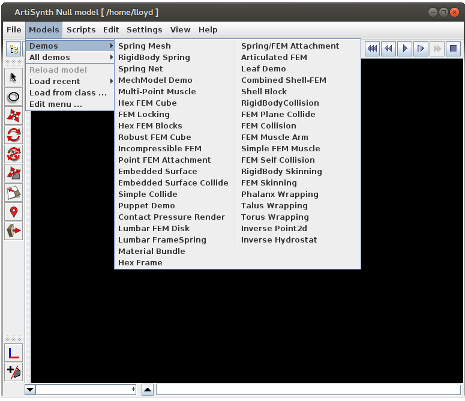
\includegraphics[]{images/ArtiSynthDemoMenu}
\else
   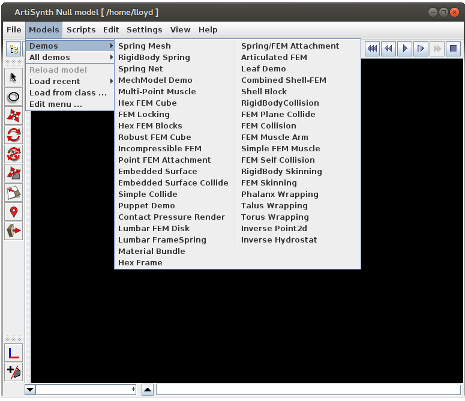
\includegraphics[width=0.65\textwidth]{images/ArtiSynthDemoMenu}
\fi
\end{center}
\caption{The ArtiSynth model selection menu.}
\label{ModelSelectionMenu:fig}
\end{figure}

Some models can be loaded directly using the {\sf Models} menu located
in the ArtiSynth menu bar (Figure \ref{ModelSelectionMenu:fig}). By
default, the upper part of this menu contains a number of submenus:

\begin{tabular}{ll} {\sf Demos} & - all models listed in the file {\tt
demoModels.txt} (described below);\\
{\sf All Demos} & - every model found in {\tt artisynth.demos} or its
subpackages, arranged hierarchically.
\end{tabular}

In addition, if {\tt artisynth\_models} has also been installed, or if
ArtiSynth otherwise detects the presence of the superpackage {\tt
artisynth.models}, then the {\sf Models} menu will also contain:

\begin{tabular}{ll} {\sf Models} & - all models listed in the file
{\tt mainModels.txt} (described below);\\
{\sf All Models} & - every model found in {\tt artisynth.models} or
its subpackages, arranged hierarchically.
\end{tabular}

Each submenu expands out to identify a set of models. Selecting one of
the models will cause it to be loaded into ArtiSynth and displayed in
the viewer. Hovering over one of the entries will display the full
classname of the associated {\tt RootModel}.  The files {\tt
demoModels.txt} and {\tt mainModels.txt} are located in the {\tt
settings} subfolder of the user configuration folder (Section
\ref{UserConfig:sec}); default instances of these are created the
first time ArtiSynth is run, and they can later be modified by the
user.

The lower part of the model menu, beneath the separator, contains
entries for reloading recent models (Section \ref{LoadingRecent:sec}),
loading a model from an explicitly specified class (Section
\ref{LoadingByClass:sec}), and customizing the upper part of the the
model menu (Section \ref{CustomizingMenus:sec}).

\begin{sideblock}
Model menu customization is is needed to create menu entries for root
models not defined within (or beneath) the packages {\tt
artisynth.demos} or {\tt artisynth.models}.
\end{sideblock}

\subsection{Loading directly by class}
\label{LoadingByClass:sec}

As mentioned above, models are defined by subclasses of 
\javaclass[artisynth.core.workspace]{RootModel}.
A model may therefore be loaded into ArtiSynth by
directly specifying the class that defines its {\tt RootModel}.  To do
this, choose {\sf ``Load from class ...''} from the lower part
of the model menu, 
which will bring up a model selection dialog as shown in Figure
\ref{modelClassSelector:fig}.

\begin{figure}[h]
\begin{center}
\iflatexml
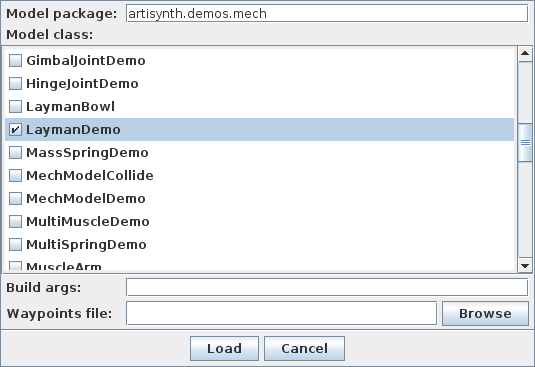
\includegraphics[]{images/modelClassSelector}
\else
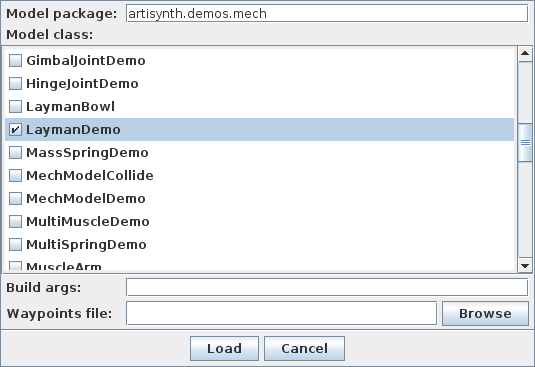
\includegraphics[width=4in]{images/modelClassSelector}
\fi
\end{center}
\caption{Dialog for selecting a model class.}%
\label{modelClassSelector:fig}
\end{figure}

Users should specify the name of the package containing the model in
the {\sf ``Model package''} field at the top. Using the {\tt <TAB>}
character in this field will invoke auto-completion based on currently
know packages, while repeated use of either {\tt <TAB>} or the up/down
arrows will scroll through known packages. Package entry is completed
using the {\tt <ENTER>} key, and any models that appear in that
package (but not its subpackages) will then be displayed in the {\sf ``Model
class''} panel below it. The user can then select the desired model by
clicking on it. In Figure \ref{modelClassSelector:fig}, the model
defined by the class {\tt artisynth.demos.mech.LaymanDemo} has been
selected.

If the model requires command-line style arguments to its {\tt
build()} method (as described in the section ``Implementing the
build() method'' of the \artisynthManual{modelguide}{ArtiSynth
Modeling Guide}), these can be entered in the {\sf ``Build args''}
field near the dialog bottom.  Arguments should be separated by white
space, with those containing white space placed between double
quotes `{\tt "}'.  The last field, {\sf ``Waypoints file''}, can
optionally be used to specify a file containing simulation way points
(Section \ref{Waypoints:sec}).  As with all externally loaded waypoint data, the
waypoints must match the current model structure.

When all desired settings have been made, the model can be loaded by
clicking the {\sf Load} button.

\subsection{Loading from a file}
\label{LoadingByFile:sec}

Finally, it is possible to load a model from a file.  Selecting {\sf
``Load model ...''} from the {\sf File} menu will bring up a File browser
that lets you select and load a model from an ArtiSynth model file.
ArtiSynth model files are text-based documents that contain a
hierarchical description of all the model's components, and are
typically identified by the extension {\tt .art}.

\begin{sideblock}
When loading a model from a {\tt .art} file, it is necessary to have
all classes associated with that model in the current Java classpath.
This can be an issue when loading files generated by other users using
application-specific Java code. Two possible solutions to this are:
(a) bundling the application-specific code into a {\tt .jar} file and
adding it to the external classpath (Section
\ref{externalClassPath:sec}), or (b) making sure that the file was
saved using only {\tt artisynth\_core} components, as described in
Section \ref{SavingSec}.
\end{sideblock}

\subsection{Loading recent models}
\label{LoadingRecent:sec}

After a model has been loaded by any of the methods described above,
it can be reloaded by selecting {\sf ``Reload model''} from the lower part
of the model menu. Models which have been recently loaded can be
reloaded by selecting {\sf ``Load recent''} from the {\sf Models} menu.

\subsection{Setting a startup model}

When working repeatedly with a specific model, it can be useful to set
that model to automatically load when ArtiSynth starts up. This can be
done by setting the {\it startup model}, by choosing {\sf ``Startup
model ...''} from the {\sf Settings} menu. This will open a
startup model dialog as shown in Figure
\ref{startupModelDialog:fig}.

\begin{figure}[h]
\begin{center}
\iflatexml
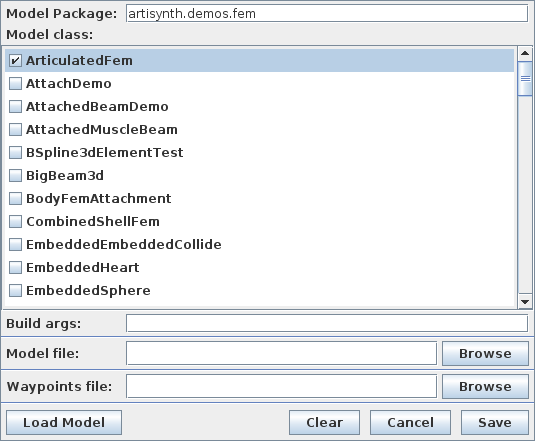
\includegraphics[]{images/startupModelDialog}
\else
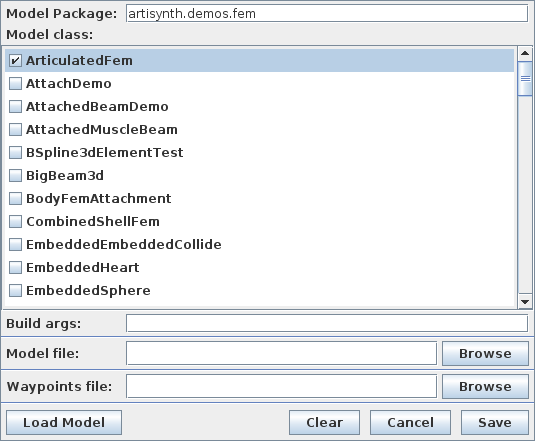
\includegraphics[width=4in]{images/startupModelDialog}
\fi
\end{center}
\caption{Dialog to set the startup model.}%
\label{startupModelDialog:fig}
\end{figure}

The model to load can be specified either by class or by file. To
specify the model by class, one uses the {\sf ``Model package''},
{\sf ``Model class''} and {\sf ``Build args''} fields to choose the
model class and optional {\tt build()} method arguments in
the same manner as described in Section \ref{LoadingByClass:sec}. To
specify the model by file, one instead uses the {\sf ``Model file''}
field to select a model file, as described in Section
\ref{LoadingByFile:sec}.

For either kind of model, it is also possible to use the {\sf
``Waypoints file''} field to specify a file of saved waypoints to be
loaded along with the model. As with all externally loaded waypoint
data, the waypoints must match the current model structure.
Waypoints are described in Section \ref{Waypoints:sec}.

\begin{itemize}

\item To save the startup model, click the {\sf Save} button at the
bottom of the dialog.

\item To clear the startup model (so that no model is loaded), click
the {\sf Clear} button followed by the {\sf Save} button.

\item To load a specified model immediately, click the {\sf Load
Model} button.

\end{itemize}

\subsubsection{Specifying models from the command line}

As an alternative to setting the startup model, one may instead use
the {\tt -model <classOrFileName>} command line option to specify a
model to load when ArtiSynth starts up. This can be useful when
running ArtiSynth from a script.  The {\tt <classOrFileName>} argument
may be either a class name or a {\tt .art} file name. If a class name
is specified and {\tt build()} method arguments are also required,
these may be listed within square brackets ({\tt [ ]}) separated by
white space. For example, to load the model class {\tt
projects.MyModel} and pass it the {\tt build()} arguments ``{\tt -size
50}'', one can invoke ArtiSynth from the command line using
%
\begin{verbatim}
> artisynth -model projects.MyModel [ -size 50 ]
\end{verbatim}
%

Models specified from the command line override the specified startup
model. To ensure that {\it no} model is loaded, one may specify
%
\begin{verbatim}
> artisynth -model none
\end{verbatim}
%

\subsection{Simulating a model}
\label{SimulatingSec}

Once a model is loaded, simulation of the model can be started,
paused, single-stepped, or reset using the play controls (Figure
\ref{PlayControlsFig}) located at the upper right of the ArtiSynth
window frame. Play controls are discussed in more detail in Section
\ref{PlayControlsSec}.

\begin{figure}[h]
\begin{center}
\iflatexml

\includegraphics[]{images/playControls}
\else

\includegraphics[width=2.5in]{images/playControls}
\fi
\end{center}
\caption{The ArtiSynth play controls. From left to right: step size
control, current simulation time, and the reset, skip-back,
play/pause, single-step, skip-forward and stop-all buttons.}%
\label{PlayControlsFig}
\end{figure}

Play controls are also available in the ArtiSynth timeline (Section
\ref{TimelineSec}).  Also, hitting the `{\tt p}', `{\tt s}'
and `{\tt r}' keys from within the viewer (Section
\ref{keyShortcutsSec}) can be used to play/pause, single step and
reset the simulation.


\subsection{Other toolbar controls}

The ArtiSynth application contains a toolbar that runs along the top
of the frame. The right side contains the play controls shown in
Figure \ref{PlayControlsFig}.

When a grid is enabled in the viewer (Section \ref{ViewerGrid}), a
text box appears in the center of the toolbar displaying the current
grid units (Section \ref{GridUnits}).

The left side of the toolbar contains the following buttons:

\begin{tabular}{l l l}
\iflatexml
\includegraphics{images/navpanelIcon}
\else
\includegraphics[width=.33in]{images/navpanelIcon}
\fi
& NavPanel: &
Shows or hides the navigation panel (Section \ref{navPanelSec})\\
\iflatexml

\includegraphics{images/resetState}
\else

\includegraphics[width=.33in]{images/resetState}
\fi
& Reset state: &
Resets the simulation state at time 0 to the current state.\\
\iflatexml
\includegraphics{images/rerender}
\else
\includegraphics[width=.33in]{images/rerender}
\fi
& Rerender: &
Rerenders all viewers and displays.\\
\iflatexml

\includegraphics{images/realtimeEnable}
\else

\includegraphics[width=.33in]{images/realtimeEnable}
\fi
& Enable real-time: &
If pressed (the default setting), forces simulations to run 
no faster than real time.
\end{tabular}

\begin{sideblock}
If real-time is enabled (via the last button), the ArtiSynth scheduler
will try to make the apparent simulation speed equal to real time.
Simulations can of course run much slower than real time if they
involve complex models with many degrees of freedom (such as large
finite element models). However, for simpler models, real-time can
also {\it increase} the overall simulation time, which is why the
option to disable real-time is provided.
\end{sideblock}

\subsection{Saving a model}
\label{SavingSec}

An ArtiSynth model can be saved to a file to be reloaded and used
later.  Selecting {\sf ``Save model as ...''} from the {\sf File} menu
will bring up a dialog that lets you select the name and directory for
the model file (Figure \ref{saveModelDialog:fig}).  If a model file
has already been specified, then one can save to it again by selecting
the {\sf Save model} menu item.  ArtiSynth model files are text-based
and are typically identified by the extension {\tt .art}.

\begin{figure}[h]
\begin{center}
\iflatexml
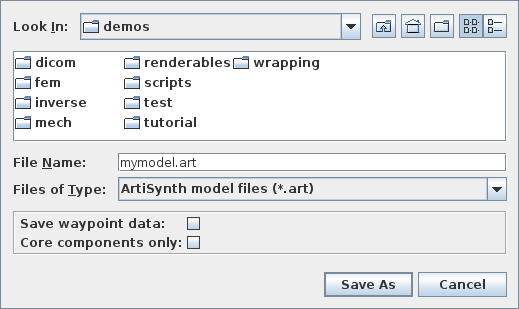
\includegraphics[]{images/saveModelDialog}
\else
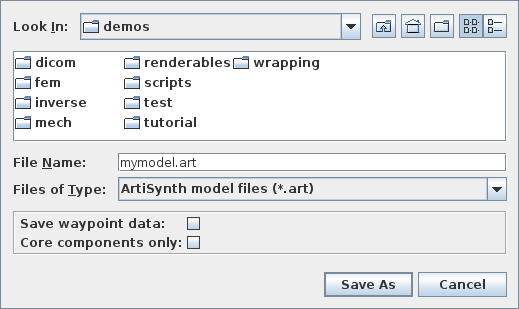
\includegraphics[width=.7\textwidth]{images/saveModelDialog}
\fi
\end{center}
\caption{The save model dialog.}%
\label{saveModelDialog:fig}
\end{figure}

When using the {\sf ``Save model as ...''} menu item, the user may choose
the following options:

\begin{description}

\item[Save waypoint data:] \mbox{}

Causes the state data for any valid waypoints (Section
\ref{waypointsSec}) to be saved (within the file) in addition to the
waypoint locations.  This is optional because a large number of
waypoints may significantly increase the file size for models with a
large state sizes.

\item[Core components only:] \mbox{}

Saves only those components which are
present in the main {\tt artisynth\_core} package. Any non-core
components, and any other components which have a hard dependency on
them, will not be written, and the user will be advised of this via a
message dialog.  The root model (Section \ref{hierarchySec}) is saved
as a pure instance of {\tt RootModel}, instead of the
application-specific class that was used to build it. This means that
any properties or class overrides specific to the application root
model class will not be present in the saved model. The advantage to
storing a model using only core components is that it can be loaded by
any {\it other} user running the same ArtiSynth version, without needing
access to any application-specific classes.

\end{description}

\subsection{Setting the external classpath}
\label{externalClassPath:sec}

As mentioned above, the classpath(s) for models declared {\it outside}
of {\tt artisynth\_core} must be made visible to ArtiSynth so that
they can be found and loaded. Detailed information on this topic is
given in the section ``Making external models visible to ArtiSynth''
of the ArtiSynth Installation Guide.

An easy way to make classpaths visible to ArtiSynth is to add them to
the {\it external classpath}, which is a list of top-level class
folders and/or {\tt .JAR} files containing the classes required to run
external models. These may include both model classes and any external
Java libraries that they require.

The external classpath is contained in a file named {\tt EXTCLASSPATH}
in the user configuration folder (Section \ref{UserConfig:sec}). This
file can be edited directly from ArtiSynth by selecting {\sf ``External
classpath ...''} from the {\sf Settings} menu, which will open the
editing dialog shown in Figure \ref{externalClasspathEditor:fig}.

\begin{figure}[h]
\begin{center}
\iflatexml
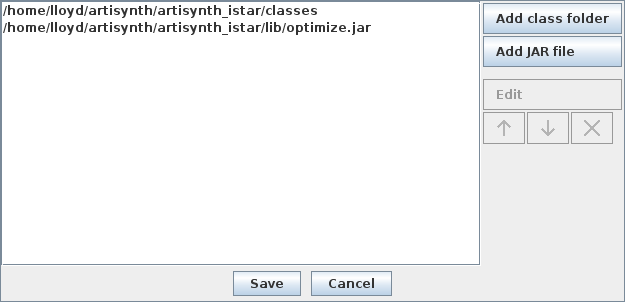
\includegraphics[]{images/externalClasspathEditor}
\else
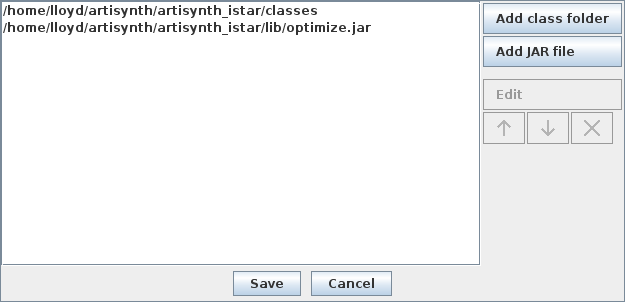
\includegraphics[width=5in]{images/externalClasspathEditor}
\fi
\end{center}
\caption{The external classpath editor.}%
\label{externalClasspathEditor:fig}
\end{figure}

The current class folders and {\tt JAR} files are listed, one per
line, in the large panel at the left. If the external classpath is
empty, this panel will be blank. New class folders or {\tt JAR} files
can be added using the {\sf ``Add class folder''} and {\sf ``Add JAR file''}
buttons at the right, which invoke file choosers appropriate to the
file type. Existing entries can be selected and then edited, moved up
or down in the list (using the up/down arrow buttons), or deleted
(using the {\sf X} button). When editing is complete, the updated
external classpath can be saved using the {\sf Save} button at the
bottom.

\begin{sideblock}
ArtiSynth must be restarted for external classpath changes to come
into effect.
\end{sideblock}

\subsection{The ArtiSynth working folder}
\label{workingDir:sec}

ArtiSynth maintains the notion of a {\it working folder}, which is
the default folder (or directory, in Unix parlance) under which the
files used to store various types of model information are stored.
This includes model files, as described above, along with other files
such as those used to store waypoints, probe configurations, or probe
data (Section \ref{savingLoadingProbes:sec}).

Chooser dialogs for these files will generally be initialized to the
working folder if their files have not been previously set.

The working folder is initialized to the system working folder from
which the ArtiSynth application is started. Once ArtiSynth is running,
it can be set by choosing {\sf ``Set working folder ...''} from the
{\sf File} menu, or by calling
\begin{verbatim}
   ArtisynthPath.setWorkingFolder (file)
\end{verbatim}
in code. When a model is saved (Section \ref{SavingSec}), the working
folder is saved with it and restored when the model file is
subsequently loaded.

\section{The Viewer}

The viewer provides interactive graphical rendering of the ArtiSynth
model and permits selection of its components. A viewer is integrated
into the ArtiSynth main frame; additional viewers can be created
if necessary.

\subsection{Viewer Toolbar}

Each viewer is provided with a toolbar (Figure \ref{ViewerToolbarFig}) equipped
with icons for controlling the viewpoint (Section \ref{ViewpointControlSec}) and
clipping planes (Section \ref{ClippingPlanesSec}). The toolbar for the main viewer
appears vertically at the lower left of the main frame, while toolbars
for additional viewers appear horizontally at the top.  Each is an
instance of Java's {\tt JToolBar}, and so can be moved and docked
accordingly.

\begin{figure}[h]
\begin{center}
\iflatexml
\includegraphics[]{images/viewerToolbar}
\else
\includegraphics[width=2.5in]{images/viewerToolbar}
\fi
\end{center}
\caption{The viewer toolbar.}%
\label{ViewerToolbarFig}
\end{figure}

\subsection{Viewpoint control}
\label{ViewpointControlSec}

The viewpoint can be controlled interactively using mouse drag
actions. There are three such actions:

\begin{description}

\item[Rotate] \mbox{}

Rotates the viewpoint about the viewer center point. By default, this
rotation is constrained so the viewer ``up'' direction remains
vertical in the view plane, but this can be changed using the viewer's
{\sf rotationMode} property (Section \ref{viewerSettings:sec}).

\item[Translate] \mbox{}

Translates the viewpoint in a plane perpendicular to the
line of sight.

\item[Zoom] \mbox{}

Zooms in or out by moving the viewpoint along the line of sight.

\end{description}

The mouse button and modifier key combinations required to effect
these actions depend on the application's {\it mouse bindings}, which
by default are set to either {\sf ThreeButton}, {\sf TwoButton}, or
{\sf OneButton} depending on the number of available mouse buttons.
Button/key combinations for each of these is described in the
following table,
%
\begin{center}
\begin{tabular}{|l|l|l|l|}
\hline
Action & {\sf ThreeButton} & {\sf TwoButton} & {\sf OneButton}\\
\hline
Rotate & 
{\tt MMB} & 
{\tt LMB}+{\tt ALT} & 
{\tt LMB}+{\tt ALT}\\
Translate & 
{\tt MMB}+{\tt SHIFT} & 
{\tt LMB}+{\tt ALT}+{\tt SHIFT} & 
{\tt LMB}+{\tt ALT}+{\tt SHIFT}\\
Zoom & 
{\tt MMB}+{\tt CTRL} & 
{\tt LMB}+{\tt ALT}+{\tt CTRL} & 
{\tt LMB}+{\tt ALT}+{\tt CTRL}\\
\hline
\end{tabular}
\end{center}
%
where {\tt MMB} and {\tt LMB} denote the {\it middle} and {\it left}
mouse buttons. If a mouse wheel is present, then this can also be used
to execute zoom actions.

\begin{sideblock}
Mouse bindings can also be set explicitly by the user and alternative
bindings are available; see Section \ref{MouseBindingsSec}.
\end{sideblock}

\label{axisAlignedViewpointsSec}
Predetermined viewpoints can also be selected using the {\it align
axis} button located on the viewer control bar.  Clicking on this
button produces a popup icon menu showing six different axis-aligned
views.  Each view is indicated by the two axes perpendicular to the
line of sight, with the X, Y, and Z axes illustrated by red, green,
and blue lines respectively. Some examples are:

%\begin{description}

\begin{tabular}{l l l}
\iflatexml
\includegraphics[]{images/alignFront}
\else
\includegraphics[width=.33in]{images/alignFront}
\fi
& Front: & Z axis up, X axis to the right.\\
\iflatexml
\includegraphics[]{images/alignBack} 
\else
\includegraphics[width=.33in]{images/alignBack} 
\fi
& Back: & Z axis up, X axis to the left.\\
\iflatexml
\includegraphics[]{images/alignTop} 
\else
\includegraphics[width=.33in]{images/alignTop} 
\fi
& Top: & Y axis up, X axis to the right.\\
\iflatexml
\includegraphics[]{images/alignBottom} 
\else
\includegraphics[width=.33in]{images/alignBottom} 
\fi
& Bottom: & Y axis down, X axis to the right.\\
\iflatexml
\includegraphics[]{images/alignLeft} 
\else
\includegraphics[width=.33in]{images/alignLeft} 
\fi
& Left: & Z axis up, y axis to the right.\\
\iflatexml
\includegraphics[]{images/alignRight} 
\else
\includegraphics[width=.33in]{images/alignRight} 
\fi
& Right: & Z axis up, y axis to the left.
\end{tabular}
%\end{description}

The align axis button itself displays the most recently selected
axis-aligned view, and the popup menu shows this view together with
five alternates which are chosen based on the current view.
Reselecting the current view will realign the viewer's viewpoint to
the current view; hitting the `{\tt v}' key from within the viewer
(Section \ref{keyShortcutsSec}) will do the same.

\subsection{Adding additional viewers}

Additional viewers can be created by selecting {\sf View > New viewer}
from the main menu. Each viewer provides independent viewing and
selection control for the current model.

%\begin{sideblock}
%We are considering adding an option whereby the main viewer can
%be split into four independent viewing panels, providing
%orthogonal projections of the front, side, and top, along
%with a general perspective projection. This arrangement is common
%in CAD and geometric modeling applications.
%\end{sideblock}

\subsection{World coordinate axes}
\label{worldCoordAxes:sec}

Hitting the 'a' key from within the viewer enables or
disables drawing of the world coordinate axes. By default, these are
drawn as simple lines, with the $x$, $y$ and $z$ axes colored red,
green and blue, respectively, and the axis length computed
automatically based on the model size.

\begin{figure}[h]
\begin{center}
\begin{tabular}{c c}
\iflatexml
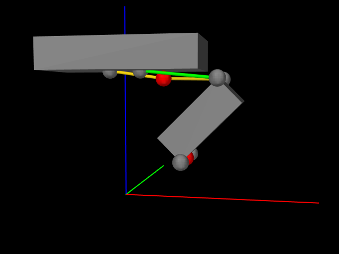
\includegraphics[]{images/viewerLineAxes} &
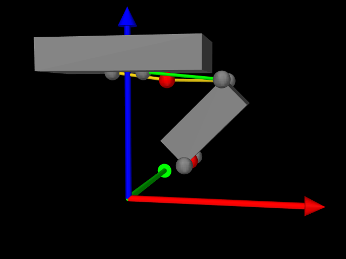
\includegraphics[]{images/viewerArrowAxes}
\else
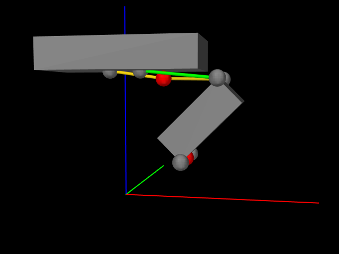
\includegraphics[width=3.2in]{images/viewerLineAxes} &
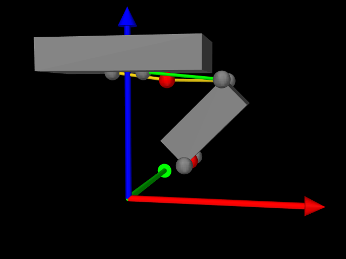
\includegraphics[width=3.2in]{images/viewerArrowAxes}
\fi
\end{tabular}
\end{center}
\caption{RigidBodyDemo with world coordinate axes drawn
as simple lines (left) and solid arrows (right).}%
\label{worldCoordAxes:fig}
\end{figure}

Axes can also be rendered as solid arrows by setting the {\sf
axisDrawStyle} property (Section \ref{viewerSettings:sec}) to {\tt
ARROW} instead of {\tt LINE}, and the axis length can be set
explicitly using the {\sf axisLength} property (Section
\ref{ViewerSpecificProps:sec}). Axes are not drawn if either {\sf
axisLength} is 0 {\it or} {\sf axisDrawStyle} is set to {\sf OFF}.

\subsection{Orthographic vs. perspective projection}
\label{ProjectionSec}

The user can toggle between orthographic and perspective projection by
selecting {\sf View > Orthographic view} or {\sf View > Perspective
view} from the main menu. Toggling can also be achieved using the
`{\tt o}' key shortcut (Section \ref{keyShortcutsSec}) within the
viewer.

\subsection{Viewer grid}
\label{ViewerGrid}

Hitting the `{\tt g}' key within the viewer enables or disables a grid
(Figure \ref{viewerGridFig}). Grid cells are square and appear in two
resolutions, with {\it major cells} subdivided into a number of {\it
minor cells}. Major cells are typically rendered more brightly than
minor cells. By default, the grid computes the cell sizes
automatically based on the current viewer zoom-level. However, it is
possible to set an explicit grid resolution (see
\ref{GridUnits}).

The grid is located in the plane perpendicular to the line of sight of
the most recently selected axis-aligned view. To change the grid
plane, select a new axis aligned viewpoint (Section
\ref{axisAlignedViewpointsSec}).

\begin{figure}
\begin{center}
\iflatexml
\includegraphics[]{images/viewerGrid}
\else
\includegraphics[width=0.66\textwidth]{images/viewerGrid}
\fi
\end{center}
\caption{Viewer showing the grid.}%
\label{viewerGridFig}
\end{figure}

\subsubsection{Grid units}
\label{GridUnits}

When the grid is enabled, a box labeled {\sf Grid:} appears in the
toolbar on top of the main ArtiSynth frame which gives the current
resolution of the grid, displayed as {\tt S/N}, where {\tt S} is the
size of each major grid cell and {\tt N} is the number of subdivisions
per cell. If there are no subdivisions, then the {\tt /N} is omitted.
For example, in Figure \ref{viewerGridFig}, this appears as {\tt Grid:
1/10}, which means that the major grid cells have a size of 1.0 and
are each divided into 10 subdivisions. The numeric value of the ratio
{\tt S/N} gives the minor cell size.

By default, the grid automatically resizes itself to the current
viewer zoom level, choosing well-rounded numbers for the grid cell
size. Auto-sizing can be enabled or disabled by right-clicking on the
{\tt Grid:} label and choosing {\sf Turn auto-sizing on} or {\sf Turn
auto-sizing off}, as appropriate. The user can also specify an
explicit value for the grid resolution by entering the desired {\tt
S/N} value (or just an {\tt S} value) into the {\tt Grid:} box.
Specifying an explicit value will disable auto-sizing, unless {\tt S}
is specified as 0 or the special value {\tt *} is entered, both of
which will re-enable auto-sizing.

\subsubsection{Axis labeling}
\label{AxisLabels}

Hitting the `{\tt l}' key within the viewer enables or disables
labeling of the major divisions along the horizontal and vertical axis
(Figure \ref{gridLabels:fig}). The division lines along which these
labels appear are automatically adjusted so as to ensure proper label
visibility, and do not necessarily correspond to the x, y, or z axes.

\begin{figure}[h]
\begin{center}
\iflatexml
\includegraphics[]{images/gridLabels}
\else
\includegraphics[width=0.66\textwidth]{images/gridLabels}
\fi
\end{center}
\caption{Viewer grid with axis labels visible.}%
\label{gridLabels:fig}
\end{figure}

It is possible to control various properties associated with
axis labeling, such as which axes are labeled, and the label size and
color. See the next section on {\sf Grid properties}.

\subsubsection{Grid properties}
\label{GridProperties}

The grid has a number of properties that can be set by right-clicking
in the viewer and choosing {\sf Set viewer grid properties} (or by
right-clicking on the {\tt Grid:} label and choosing {\sf Set
properties}). This will bring up a property dialog, such as that shown
in Figure \ref{GridPropDialog:fig}.

\begin{figure}
\begin{center}
\iflatexml
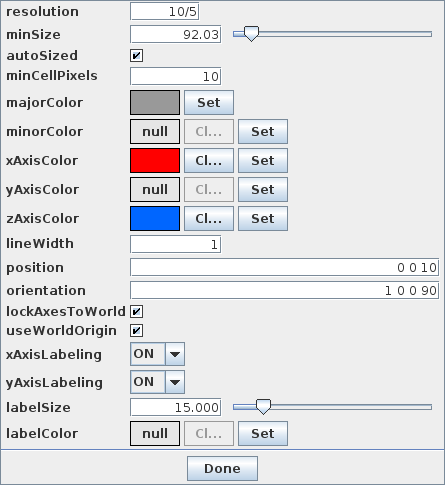
\includegraphics[]{images/gridPropDialog}
\else
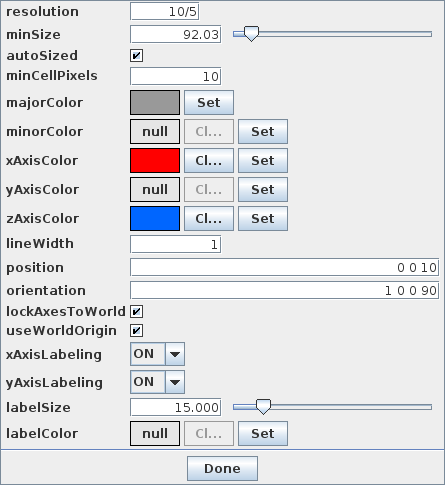
\includegraphics[width=0.5\textwidth]{images/gridPropDialog}
\fi
\end{center}
\caption{Dialog to control the grid properties.}%
\label{GridPropDialog:fig}
\end{figure}

Properties that can be set include:

\begin{description}

\item[resolution]\mbox{}

Grid resolution, as described above.

\item[autoSized]\mbox{}

If {\tt true}, causes the grid resolution to be recomputed as the user
adjusts the view position, orientation, and zoom.

\item[minCellPixels]\mbox{}

Minimum number of pixels that should appear in a minor cell division
when autosizing.

\item[majorColor]\mbox{}

Color to use for the major axis lines.

\item[minorColor]\mbox{}

Color to use for the minor axis lines.

\item[xAxisColor]\mbox{}

Color to use for the grid line that corresponds to the world y axis,
or the horizontal axis if {\sf lockAxesToWorld} is false.

\item[yAxisColor]\mbox{}

Color to use for the grid line that corresponds to the world y axis,
or the vertical axis if {\sf lockAxesToWorld} is false.

\item[zAxisColor]\mbox{}

Color to use for the grid line that corresponds to the world z
axis.

\item[lineWidth]\mbox{}

Width of the grid lines, in pixels.

\item[position]\mbox{}

Translation position of the grid, in world coordinates.

\item[orientation]\mbox{}

Orientation of the grid, in world coordinates.

\item[lockAxesToWorld]\mbox{}

If {\tt true}, forces the grid to stay aligned with the orientation
and position of the world axes. In particular, the horizontal and
vertical axes will always be parallel to one of the x, y, or z world
axes, the grid center will be a multiple of major cell sizes from the
origin, and axis labels will be set relative to the world origin.

\item[useWorldOrigin]\mbox{}

If {\tt true}, causes the principal horizontal and vertical axes to be
aligned with the world origin. Otherwise, the axes will be aligned
with the grid center. This property can only be {\tt true} if {\sf
lockAxesToWorld} is also {\tt true}.

\item[xAxisLabeling]\mbox{}

Enables labeling of the x axis.

\item[yAxisLabeling]\mbox{}

Enables labeling of the y axis.

\item[labelSize]\mbox{}

'em' size of the label text, in pixels.

\item[labelColor]\mbox{}

If set, specifies the color used to draw the label text. Otherwise,
the major axis color is used.

\end{description}

\subsection{Clipping planes}
\label{ClippingPlanesSec}

The user can add clipping planes to the viewer. These are useful for
restricting what is rendered and allowing a better view of interior
structures, as shown in (Figure \ref{clipPlaneFig}).

\begin{figure}
\begin{center}
\iflatexml
\includegraphics[]{images/clipPlane}
\else
\includegraphics[width=0.66\textwidth]{images/clipPlane}
\fi
\end{center}
\caption{Clipping plane showing interior of tongue model (left), disabled (center), and in slice mode (right).}%
\label{clipPlaneFig}
\end{figure}

\subsubsection{Adding and removing}

To add a clipping plane, left click on the {\sf add clip plane}
button \includegraphics[width=.25in]{images/addClipPlane} located on the
viewer toolbar. This will create a clipping plane located in the plane
perpendicular to the current line of sight.

It will also add to the viewer toolbar a {\sf clip plane} icon
\includegraphics[width=.25in]{images/clipPlaneIcon} for controlling the
clipping plane. Right-clicking on this icon will bring up an option
menu.

To delete a clipping plane, right-click on its icon and
select {\sf Delete}.

\subsubsection{Moving}

A clip plane is associated with a coordinate system and can be moved
and/or rotated by dragging on the trans-rotate transformer located at
its coordinate system origin. The clip region is the half space lying
in the direction of the +z axis.

The transformer itself can be made invisible/visible by right-clicking
on the clip plane icon and selecting {\sf Hide transformer} or {\sf Show
transformer}.

\subsubsection{Offsets}

The clipping region is the half space lying in the direction of the +z
axis of the plane's local coordinate system. By default, clipping is
actually offset by a small distance along the +z axis, so that small
objects (such as points) lying in the x-y plane remain
visible. The amount of this offset is controlled by the plane's
{\sf offset} property, which is set to a nominal default value. To control
this property directly, right-click on the clip plane icon and select
{\sf Set properties}. This will bring up a panel which allows the offset
to be adjusted.

\subsubsection{Enabling/disabling}

Left clicking on the clip plane icon will enable/disable
clipping. Disabling clipping allows the plane to be used as a regular
movable grid. When clipping is disabled, the icon
will change to the form
\includegraphics[width=.25in]{images/clipPlaneOffIcon}.

\subsubsection{Slicing mode}

Clipping planes can be placed in a {\it slicing mode}, whereby half-spaces
in both the positive and negative z directions are clipped. The result
is a small slice about the local x-y plane (Figure \ref{clipPlaneFig},
right). The width of this slice is controlled by the plane's {\sf offset}
property, as described above.

To enable or disable slicing, right-click on the clip plane icon
and select {\sf Enable slicing} or {\sf Disable slicing}.

\subsubsection{Other features}

\begin{description}

\item[Properties]\mbox{}

Various properties associated with the plane, such as its color, line
width, cell resolution, etc., can be set explicitly by the user. To do
this, right-click on the icon, select {\sf Set properties}, and edit
the resulting property panel.  Most properties are the same as those
described for the main viewer grid in \ref{GridProperties}.

\item[Grid visibility]\mbox{}

To make the grid invisible/visible, right-click on the icon
and select {\sf Hide grid} or {\sf Show grid}.

\item[Alignment with world axes]\mbox{}

The clip plane can be aligned so that it's
normal lies along the positive or negative direction of either the x,
y, or z world axes. Right-click on the icon and select the
appropriate option. Clipping is performed so that
the half-space lying in the direction of the normal is clipped.

\item[Alignment with current line of sight]\mbox{}

To align the clipping plane so that it is perpendicular to the
current line of sight, right-click on the icon and select {\sf Reset}.

\end{description}

\subsection{Indicating 3D positions with the mouse}
\label{indicatingPositionsSec}

It is possible to use a viewer in combination with a mouse to specify the
position of a 3D point in space. This is commonly employed in the
editing operations described in Section \ref{componentEditingSec}.

To specify a point, the user left-clicks the mouse in the viewer, at
the screen position located over the point's desired position. The 3D
position is then determined by intersecting the ray indicated by the
mouse clock with some appropriate surface or plane. Typically, a plane
perpendicular to the viewing direction and passing through the model's
center is used. Alternatively, some interactions provide a {\sf constrain
to plane} option, which causes the ray to be intersected with a viewer
clipping plane (Section \ref{ClippingPlanesSec}), providing more precise control
over the point's position. This requires that the viewer presently
contain at least one clipping plane. If more than one clipping plane
is present, the first one is used.

In other applications, the desired point may be known to lie on a 3D
surface, in which case the position is determined by intersecting the
ray with a 3D surface mesh.

\subsection{Viewer properties}
\label{viewerSettings:sec}

Viewers export a number of properties that control various aspects of
their look and feel. Some of these can be modified collectively for
all viewers by choosing {\sf ``Settings > Viewers ...''} from the
main menu, which opens a {\it viewer settings} dialog (Figure
\ref{viewerSettingsDialog:fig}).

\begin{figure}[h]
\begin{center}
\iflatexml
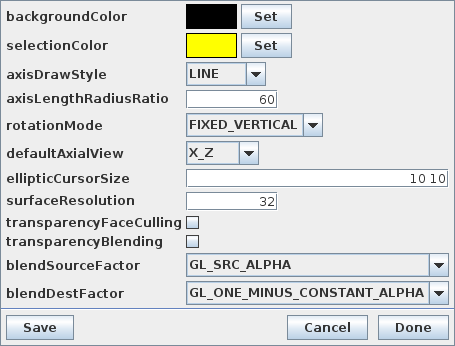
\includegraphics[]{images/viewerSettings}
\else
\includegraphics[width=3.5in]{images/viewerSettings}
\fi
\end{center}
\caption{Viewer settings dialog.}%
\label{viewerSettingsDialog:fig}
\end{figure}

Various properties can be set by this dialog, as described below.
Clicking the {\sf Save} button will save the current settings to the
user's preferences (Section \ref{Preferences:sec}) so that they will
be set automatically when ArtiSynth is restarted.

Properties set by the viewer settings dialog include:

\begin{description}

\item[backgroundColor]\mbox{}

Color of the viewer background.

\item[selectionColor]\mbox{}

Color used to highlight selected items.

\item[axisDrawStyle]\mbox{}

Controls how world coordinate axes are drawn (Section
\ref{worldCoordAxes:sec}), with {\sf LINE} and {\sf ARROW} specifying
simple lines and solid arrows, respectively.

\item[axisRadiusRatio]\mbox{}

A ratio which can be used to determine the radius for an axis when the
radius is not explicitly specified. The radius is computed by
multiplying the ratio by the axis length. This is typically used when
rendering coordinate axes as solid arrows and has a default value of
0.016.

\item[rotationMode]\mbox{}

Controls how the eye-to-world rotation is adjusted when the mouse is
used to perform a rotate action (Section \ref{ViewpointControlSec}).
The default value is {\sf FIXED\_VERTICAL}, which constrains the
viewer's ``up'' vector to remain vertical with respect to the view
plane, at the expense of preventing the eye-to-world rotation from
being adjustable to an arbitrary value. Alternate values include {\sf
CONTINUOUS}, which enables a track-ball type rotation that does allow
arbitrary adjustment of the eye-to-world rotation, and {\tt OFF},
which disables rotation adjystment.

\item[defaultAxialView]\mbox{}

Sets the default axis alignment indicating how the 3D world axes
correspond to the horizontal ``right'' and vertical ``up'' view plane
directions.  Each setting takes the form $R$\_$U$, where $R$ is the
world axis pointing right and $U$ is the axis pointing up, and $R$ and
$U$ can each be either {\tt X}, {\tt Y}, {\tt Z}, {\tt NX}, {\tt NY},
or {\tt NZ}, indicating the positive or negative $x$, $y$ or $z$ axis.

\item[ellipticCursorSize]\mbox{}

Size of the elliptic cursor (Section \ref{ellipticSelection:sec}) in
the horizontal and vertical directions. The default value is
$(10, 10)$.

\item[surfaceResolution]\mbox{}

Controls the number of faces or segments used for
rendering built-in curved primitives, such as cylinders and
spheres. For cylinders, it controls the number of sides, while for
spheres it controls the number of longitudinal slices. A larger number
produces a smoother effect at increased graphical cost. The default
value is 32.

\end{description}

For OpenGL based viewers, the following properties are also provided
to control how transparency is rendered:

\begin{description}

\item[transparencyFaceCulling]\mbox{}

Enables or disables face culling when rendering transparency.

\item[transparencyBlending]\mbox{}

Enables or disables transparency blending (via {\tt glEnable()} or
{\tt glDisable()} using {\tt GL\_BLEND}) when rendering transparency.

\item[blendSourceFactor]\mbox{}

Specifies the first (source) argument to {\tt glBlendFunc()}.

\item[blendDestFactor]\mbox{}

Specifies the second (destination) argument to {\tt glBlendFunc()}.

\end{description}

\subsubsection{Viewer-specific properties}
\label{ViewerSpecificProps:sec}

Viewer properties can also be set on a per-viewer basis. To do this,
invoke the context menu (usually right-click) in the viewer when
nothing is selected, and choose {\sf Set viewer properties}.
Individual properties include all those described above (except with
{\tt defaultAxialView} renamed to {\tt axialView}), together with the
following additional properties:

\begin{description}

\item[axisLength]\mbox{}

Axis lengths used to render the world axes (Section
\ref{worldCoordAxes:sec}).

\item[viewControlMask]\mbox{}

If set to {\tt ALONG\_X\_ONLY} or {\tt ALONG\_Y\_ONLY}, mouse-based
view control inputs are restricted to those in the x or y screen
directions, respectively. This makes it easier to limit changes in the
view point. The default value is {\tt NONE} (no restriction).

\item[eye]\mbox{}

Location of the eye position, in world coordinates.

\item[center]\mbox{}

Location of the viewing frustum center, in world coordinates.

\end{description}

\begin{sideblock}
Setting a viewer-specific property, such as the background color, will
generally cause it to have a value that differs from its counterpart
in the viewer settings (because the value was set for only a single
viewer). On the other hand, properties set in the viewer settings will
be applied to {\it all} open viewers.
\end{sideblock}

\subsection{Mouse Bindings}
\label{MouseBindingsSec}

The ArtiSynth GUI was originally designed for a three-button mouse, in
which the left button is used for selection, the middle button
controls the viewpoint, and the right button is used to activate the
context menu. These are used in conjunction with the modifier keys
{\tt SHIFT} and {\tt CTRL} to effect different actions.

For systems that do not have a three-button mouse, ArtiSynth by
default detects the number of mouse buttons and adjusts the mouse
bindings so that the {\tt ALT} key emulates the middle button and the
{\tt META} key emulates the right button.

\begin{sideblock}
The {\tt META} key is usually associated with either the {\tt COMMAND}
key (Mac) or the {\tt WINDOWS} key.
\end{sideblock}

\begin{figure}[h]
\begin{center}
\iflatexml
\includegraphics[]{images/mouseSettingsDialog}
\else
\includegraphics[width=3in]{images/mouseSettingsDialog}
\fi
\end{center}
\caption{Mouse bindings dialog.}%
\label{mouseSettingsDialog:fig}
\end{figure}

Mouse bindings can also be explicitly set by the user, by choosing
{\sf ``Settings > Mouse ...''} from the main menu, which opens a {\it
mouse bindings} dialog (Figure \ref{mouseSettingsDialog:fig}).  This
allows the user to change the bindings, and also for any given binding
describes the button/key combinations to effect various actions. If
the {\sf ``Auto detect''} checkbox is selected, then the bindings are
determined automatically from the number of available mouse buttons.
Unchecking this box allows the bindings to be set explicitly using the
{\sf Bindings} selector. The dialog also allows control of the scale
factor used for mouse wheel zoom actions.

Clicking the {\sf Save} button in the mouse bindings dialog will save
the current bindings  to the user's preferences (Section
\ref{Preferences:sec}) so that they will be set automatically when
ArtiSynth is restarted. Mouse bindings can also be specified
explicitly at startup using the {\tt -mousePrefs <bindings>} command
line option.

Currently, there are five bindings available:

\begin{description}

\item[ThreeButton]\mbox{}

Default bindings for a three-button mouse.

\item[TwoButton]\mbox{}

Default bindings for a two-button mouse. The middle mouse button
is emulated with the {\tt ALT} key.

\item[OneButton]\mbox{}

Default bindings for a one-button mouse. The middle and right mouse
buttons is emulated with the {\tt ALT} and {\tt META} keys.

\item[Laptop]\mbox{}

Legacy bindings for a two-button mouse.

\item[Mac]\mbox{}

Legacy bindings for a Mac type one-button mouse.

\end{description}

Tables showing the button and modifier key combinations that effect
different actions for each of these are given below, with {\tt LMB},
{\tt MMB}, and {\tt RMB} denoting the left, right and middle mouse
buttons.  Actions marked with an asterisk (*) are drag actions which
can have their modifier keys invoked or removed during a drag
operation. Button/key combinations for {\sf ThreeButton}, {\sf
TwoButton}, and {\sf OneButton} are:

\begin{center}
\begin{tabular}{|l|l|l|l|}
\hline
Action & {\sf ThreeButton} & {\sf TwoButton} & {\sf OneButton}\\
\hline
\hline
\multicolumn{4}{|l|}{Viewpoint control (Section \ref{ViewpointControlSec})}\\
\hline
Rotate view & 
{\tt MMB} & {\tt LMB}+{\tt ALT} & {\tt LMB}+{\tt ALT}\\
Translate view & 
{\tt MMB}+{\tt SHIFT} & {\tt LMB}+{\tt ALT}+{\tt SHIFT} & 
{\tt LMB}+{\tt ALT}+{\tt SHIFT}\\
Zoom view & 
{\tt MMB}+{\tt CTRL} & {\tt LMB}+{\tt ALT}+{\tt CTRL} & 
{\tt LMB}+{\tt ALT}+{\tt CTRL}\\
\hline
\multicolumn{4}{|l|}{Component selection (Section \ref{viewerSelectionSec})}\\
\hline
Select components & 
{\tt LMB} & {\tt LMB} & {\tt LMB}\\
Multiple selection & 
{\tt LMB}+{\tt CTRL} & {\tt LMB}+{\tt CTRL} & {\tt LMB}+{\tt CTRL}\\
Elliptic selection & 
{\tt LMB} & {\tt LMB} & {\tt LMB}\\
Elliptic deselection$^*$ & 
{\tt LMB}+{\tt SHIFT} & {\tt LMB}+{\tt SHIFT} & {\tt LMB}+{\tt SHIFT}\\
Resize elliptic cursor & 
{\tt LMB}+{\tt SHIFT}+{\tt CTRL} & {\tt LMB}+{\tt SHIFT}+{\tt CTRL} & 
{\tt LMB}+{\tt SHIFT}+{\tt CTRL}\\
Context menu & 
{\tt RMB} & {\tt RMB} & {\tt LMB}+{\tt META}\\
\hline
\multicolumn{4}{|l|}{Manipulator controls (Section \ref{TransformerToolsSec})}\\
\hline
Move dragger & 
{\tt LMB} & {\tt LMB} & {\tt LMB}\\
Dragger constrain$^*$ & 
{\tt LMB}+{\tt SHIFT} & {\tt LMB}+{\tt SHIFT} & {\tt LMB}+{\tt SHIFT}\\
Dragger reposition$^*$ & 
{\tt LMB}+{\tt CTRL} & {\tt LMB}+{\tt CTRL} & {\tt LMB}+{\tt CTRL}\\
\hline
\end{tabular}
\end{center}

while those for {\sf Laptop} and {\sf Mac} are:

\begin{center}
\begin{tabular}{|l|l|l|}
\hline
Action & {\sf Laptop} & {\sf Mac}\\
\hline
\hline
\multicolumn{3}{|l|}{Viewpoint control (Section \ref{ViewpointControlSec})}\\
\hline
Rotate view & 
{\tt LMB} & {\tt LMB}+{\tt ALT}\\
Translate view & 
{\tt LMB}+{\tt SHIFT} & {\tt LMB}+{\tt ALT}+{\tt SHIFT} \\
Zoom view & 
{\tt LMB}+{\tt ALT} & {\tt LMB}+{\tt ALT}+{\tt META} \\
\hline
\multicolumn{3}{|l|}{Component selection (Section \ref{viewerSelectionSec})}\\
\hline
Select components & 
{\tt LMB}+{\tt CTRL} & {\tt LMB} \\
Multiple selection & 
{\tt LMB}+{\tt SHIFT}+{\tt CTRL} & {\tt LMB}+{\tt META} \\
Elliptic selection & 
{\tt LMB}+{\tt CTRL} & {\tt LMB} \\
Elliptic deselection$^*$ & 
{\tt LMB}+{\tt SHIFT}+{\tt CTRL} & {\tt LMB}+{\tt SHIFT} \\
Resize elliptic cursor & 
{\tt LMB}+{\tt SHIFT}+{\tt CTRL} & {\tt LMB}+{\tt SHIFT}+{\tt CTRL}\\
Context menu & 
{\tt RMB} & {\tt LMB}+{\tt CTRL} \\
\hline
\multicolumn{3}{|l|}{Transformer control (Section \ref{TransformerToolsSec})}\\
\hline
Move dragger & 
{\tt LMB} & {\tt LMB} \\
Dragger constrain$^*$ & 
{\tt LMB}+{\tt SHIFT} & {\tt LMB}+{\tt SHIFT} \\
Dragger reposition$^*$ & 
{\tt LMB}+{\tt ALT} & {\tt LMB}+{\tt ALT} \\
\hline
\end{tabular}
\end{center}

\subsection{Keyboard shortcuts}
\label{keyShortcutsSec}

When the viewer has the keyboard focus, the following key shortcuts
are available:

\begin{center}
\begin{tabular}{|l|l|}
\hline
Key & Operation \\
\hline
{\tt q} & quit ArtiSynth \\
{\tt t} & toggle time line visibility \\
{\tt z} & undo last command \\
\hline
\multicolumn{2}{|l|}{Play controls (Section \ref{SimulatingSec}):}\\
\hline
{\tt p} or {\tt SPC} & play/pause\\
{\tt s} & single step \\
{\tt r} & reset \\
\hline
\multicolumn{2}{|l|}{Viewer controls:}\\
\hline
{\tt v} & reset view (Section \ref{ViewpointControlSec})\\
{\tt o} & toggle orthographic/perspective view 
(Section \ref{ProjectionSec})  \\
{\tt a} & toggle visibility of axes showing world coordinates\\
{\tt g} & toggle viewer grid (Section \ref{ViewerGrid})\\
{\tt l} & toggle viewer grid labels\\
\hline
\multicolumn{2}{|l|}{%
Selection and transformer (Sections \ref{viewerSelectionSec} 
and \ref{TransformerToolsSec}):}\\
\hline
{\tt ESC} & select parent of last selection\\
{\tt c} & clear selection\\
{\tt d} & reset elliptic cursor size to default\\
{\tt w} & set current transformer frame to world coordinates\\
{\tt b} & set current transformer frame to body/local coordinates\\
\hline
\end{tabular}
\end{center}

\section{Component Navigation and Selection}

An ArtiSynth model is composed of a hierarchical arrangement of
model components (each of which implements the interface 
\javaclass[artisynth.core.modelbase]{ModelComponent}), 
some of which may themselves
be models. The graphical interface allows users to navigate this
hierarchy and select individual components. Selected components
can then be edited, or have specific properties modified or attached
to probes or control panels.

\subsection{The component hierarchy}
\label{hierarchySec}

An example component hierarchy is shown in Figure
\ref{hierarchyFig}. At the top is a {\it root model} (class
\javaclass[artisynth.core.workspace]{RootModel}), 
in this case named {\tt Rigid Body Spring}.  The
root model in turn contains a list of models, one of which is a
mechanical model named {\tt msmod}, which here contains particles and
rigid bodies.

It is important to node that in the component hierarchy, any collection
of components is itself a component (usually an instance of
\javaclass[artisynth.core.modelbase]{ComponentList}). 
This provides automatic ``grouping'' of
components of like type, but does introduce additional levels into the
hierarchy. Hence the particle {\tt red} is a child not of {\tt msmod},
but rather the component list {\tt particles}.

\begin{figure}
\begin{center}
\iflatexml
\includegraphics[]{images/hierarchy}
\else
\includegraphics[width=0.66\textwidth]{images/hierarchy}
\fi
\end{center}
\caption{A sample component hierarchy.}%
\label{hierarchyFig}
\end{figure}

\subsubsection{Component names and numbers}

Model components may be assigned a string name; at the time of
this writing names may not begin with a digit, have zero length, contain
the characters `{\tt .}' or `{\tt /}', or equal the reserved word {\tt this}.
Components which do not have an assigned name are
called {\it nameless}.

All components have a {\it number}, even if they do not have a name. The
number is assigned automatically when the component is added to the
parent, and is guaranteed to be persistent until the component is
removed from the parent.

\subsubsection{Component path names}
\label{pathNamesSec}

The names and/or numbers of a component's ancestors can be used to
form a {\it component path name}. This path has a construction completely
analogous to Unix file path names, with the `{\tt /}' character acting as
a separator. Absolute paths start with `{\tt /}' and begin with the root
model. Relative paths omit the leading `{\tt /}' and can begin lower down
in the hierarchy.  The absolute path name of the {\tt red} particle in
Figure \ref{hierarchyFig} would be

\begin{verbatim}
/Rigid Body Spring/models/msmod/particles/red
\end{verbatim}

For nameless components in the path, their
numbers can be used instead:

\begin{verbatim}
 /Rigid Body Spring/models/msmod/rigidBodies/1
\end{verbatim}

Numbers can be used even for components that have names.
Hence a path name consisting only of numbers, as in

\begin{verbatim}
 /0/0/0/3/1
\end{verbatim}

is legal, although it most likely to appear only in machine-generated
output.

\subsection{Navigation panel selection}
\label{navPanelSec}

A navigation panel in the main ArtiSynth frame allows direct
navigation of the component hierarchy. The panel can be
open or closed by clicking on the main toolbar icon 
\iflatexml
\includegraphics[]{images/navpanelIcon}.
\else
\includegraphics[width=.25in]{images/navpanelIcon}.
\fi

Figure \ref{navpanelFig} shows an navigation panel containing a superset
of the hierarchy diagrammed in Figure \ref{hierarchyFig}.

\begin{figure}
\begin{center}
\iflatexml
\includegraphics[]{images/navpanel}
\else
\includegraphics[width=0.30\textwidth]{images/navpanel}
\fi
\end{center}
\caption{An typical navigation panel display.}%
\label{navpanelFig}
\end{figure}

Left clicking on any component in the navigation panel selects that
component. Clicking while pressing the {\tt CTRL} key (or the {\tt
CMD} key on some platforms, such as Mac) allows selection of multiple
components. Clicking while pressing the {\tt SHIFT} key allows
selection of a range of components.

\subsubsection{Large numbers of nameless components}

In some cases, such as finite element models, the number of child
components can be very large (on the order of thousands). In order to
keep the navigation panel size manageable, the number of nameless
children displayed is limited to a set number (currently 100).  If the
number of nameless children exceeds this number, the display will be
augmented with an expand icon {\tt >{}>{}>}. Clicking on this will expand the
display to include all nameless components, and the expand icon will
be replaced by a contract icon {\tt <{}<{}<}. Clicking on the contract icon
will cause the extra nameless components to be hidden again.
This is illustrated in Figure \ref{navpanelExpandContractFig}.

\begin{figure}
\begin{center}
\begin{tabular}{cc}
\iflatexml
  \includegraphics[]{images/navpanelCompact}&
  \includegraphics[]{images/navpanelExpand}\\
\else
  \includegraphics[width=2.25in]{images/navpanelCompact}&
  \includegraphics[width=2.25in]{images/navpanelExpand}\\
\fi
\end{tabular}
\end{center}
\caption{Expansion of nameless components in the navigation panel.}%
\label{navpanelExpandContractFig}
\end{figure}

\subsection{Viewer selection}
\label{viewerSelectionSec}

Components that are rendered in the viewer can generally be selected
by variety of methods (the exception is for a few renderable
components that do not support selection). These methods include {\it click},
{\it box}, and {\it elliptic} selection. The top two icons in the
selection toolbar at the left of the ArtiSynth frame control the
current selection method. In addition, hitting the `{\tt c}' key
from within the viewer
(Section \ref{keyShortcutsSec}) clears the current selection.

\subsubsection{Click and box selection}

Click and box selection are enabled by the arrow icon at the top of
the selection toolbar:

\vspace{\parskip}
\iflatexml
\includegraphics[]{images/selectTool}
\else
\includegraphics[width=.33in]{images/selectTool}
\fi

Click selection involves left clicking on a component, causing it to
be selected. Selection of multiple components is enabled by left
clicking with a modifier key, which is usually {\tt CTRL}
but may be different for some legacy mouse bindings 
(Section \ref{MouseBindingsSec}).

\begin{sideblock}
Click selection selects only those components which are actually
visible to the viewer; components which are hidden cannot be selected
this way.
\end{sideblock}

Box selection is effected by left-clicking and dragging in the viewer,
causing the selection of all components rendered within the resulting
drag box. Because this often results in the selection of more
components than desired, it may be useful to employ a selection filter
(Section \ref{selectionFiltersSec}). Any components within the drag
box which are already selected will be deselected.

\begin{sideblock}
Box selection acts on {\it all} (filtered) components within the view
frustum defined by the drag box, including those which are hidden
from view.
\end{sideblock}

\subsubsection{Elliptic selection}
\label{ellipticSelection:sec}

Elliptic selection is enabled by the elliptic icon near the top of
the selection toolbar:

\vspace{\parskip}
\iflatexml
\includegraphics[]{images/ellipticSelectTool}
\else
\includegraphics[width=.33in]{images/ellipticSelectTool}
\fi

This causes an additional elliptic cursor (which defaults to a circle)
to be drawn around the mouse cursor. Selection is effected by
dragging, and causes all visible objects within the ellipse to be
selected. The selection process is cumulative, with subsequent drags
selecting additional components. As with all selection operations, a
filter can be set to restrict the components that are selected
(Section \ref{selectionFiltersSec}). Generally, the drag select
operation requires no modifier keys, although it may with some legacy
mouse bindings (Section \ref{MouseBindingsSec}).

It is also possible to {\it deselect} components in the same way, by
using the {\tt SHIFT} modifier key to cause drag operations to
cumulatively deselect components.
	
\begin{sideblock}
Elliptic selection selects only those components which are actually
visible to the viewer; components which are hidden cannot be selected
this way.
\end{sideblock}

The elliptic cursor used for selection can be resized, either
interactively, or by setting the {\tt ellipticCursorSize} property of
the viewer (Section \ref{viewerSettings:sec}). To interactively change
the cursor size, initiate a drag operation with the {\tt CTRL} and
{\tt SHIFT} modifiers. Finally, the `{\tt
d}' key shortcut within the viewer will cause the cursor to be reset
to its default size.

\subsubsection{Selection filtering}
\label{selectionFiltersSec}

It is possible to limit viewer selection to components of a specific
type. This can be done using the selection filter widget at the bottom
left of the main ArtiSynth frame Figure
\ref{selectionFilterWidgetFig}.

\begin{figure}
\begin{center}
\iflatexml
\includegraphics[]{images/selectionFilterWidget}
\else
\includegraphics[width=0.40\textwidth]{images/selectionFilterWidget}
\fi
\end{center}
\caption{The selection filter widget.}%
\label{selectionFilterWidgetFig}
\end{figure}

To enable filtering, type into the widget text box the class name of
the component type you wish to restrict filtering to. It is generally
only necessary to enter the leaf name of the class (e.g., {\tt Particle}
or {\tt AxialSpring}), and the system will then find the full
class name by searching the ArtiSynth class path.

Once filtering is enabled, only components which are instances
(including subclasses) of the specified type will be selectable.

Previously selected filters can be recalled using a history
list accessible using the leftmost arrow button on the
selection widget.

To remove selection filtering, enter the special filter {\tt *}, either by
typing this in the text box, or using the history list.

\subsection{Selection display}
\label{selectionDisplaySec}

The selection display Figure \ref{selectionDisplayWidgetFig} at the bottom of the
main ArtiSynth frame shows the full path name of the last component
added to the selection list. This is useful for identifying components
in detail.

If no components are selected, then the selection display is blank.

\begin{figure}
\begin{center}
\iflatexml
\includegraphics[]{images/selectionDisplay}
\else
\includegraphics[width=0.50\textwidth]{images/selectionDisplay}
\fi
\end{center}
\caption{The selection display widget.}%
\label{selectionDisplayWidgetFig}
\end{figure}

The selection display is useful for disambiguating situations where it
is not clear what component we have actually selected in the viewer.
For example, FEM models keep their surface mesh contained within a
descendant component. Selecting the surface mesh will cause this
container component to be selected and highlighted, making it {\it
appear} as though the FEM model itself is selected rather than the
container. Checking the selection display makes it clear what
component has actually been selected. If desired, one can easily
navigate to one of the ancestor components using parent selection, as
described in the next section.

\subsection{Selecting parent and ancestor components}
\label{selectingAncestorsSec}

Sometimes, when you select a component, you actually want to select
one of it's ancestor components. 

There are several ways to do this:

\begin{enumerate}

\item Hit the escape ({\sf ESC}) key within the viewer window. This
will select the parent of the currently selected component. Hitting
escape repeatedly is a fast way to proceed up the component hierarchy.

\item Click on the ``up'' arrow located at the left of the selection
display (Figure \ref{selectionDisplayWidgetFig}). This will also
select the parent of the currently selected component.

\end{enumerate}

Parent selection is particularly useful in the commonly occurring
situation where a composite component is not rendered and therefore
not selectable in the viewer. For instance, suppose we wish to select
a FEM model. One can select any renderable descendant of the model,
such as a node, element, or its surface mesh (if displayed), and then
use repeated parent selection until the model itself is selected.

\subsection{Highlighting selected components}

Selected components are rendered in the viewer using a special
selection color (yellow at the time of this writing). It is important
to note that descendants of a selected component are {\bf not} presently
rendered in any special way. For instance, if an FEM is selected, it's
nodes and elements will be rendered normally. 

While this has the potential to be confusing, we have not yet found
this to be problematic, as the navigation panel and selection display
provide alternative indicators as to what is currently selected.

\section{Model Manipulation}
\label{ModelManipulation}

Various tools located within the selection toolbar at the left of the
main ArtiSynth frame allow models to be manipulated in various ways.
These include modifying component locations, orientations, and
geometry using the transformer tools (Section
\ref{TransformerToolsSec}), exerting point forces on selected
components using the pull controller (Section
\ref{PullControllerSec}), and adding marker points to certain
components types (Section \ref{MarkerTool}).

The behavior of these tools is somewhat context dependent.  For
example, the transformer tools will only transform those {\it
transformable} components which implement the
\javaclass[artisynth.core.modelbase]{TransformableGeometry}
interface. The behavior may also vary depending on whether or not
simulation is in progress.

\subsection{Dragger fixtures}
\label{draggerFixturesSec}

The transformation tools employ the dragger fixtures shown
in Figure \ref{transformToolsFig}, which allow 3D geometrical
transformations to be performed within the viewer.

\begin{figure}
\begin{center}
\iflatexml
\includegraphics[]{images/transformTools}
\else
\includegraphics[width=0.80\textwidth]{images/transformTools}
\fi
\end{center}
\caption{Dragger fixtures: translator, rotator, and transrotator.}%
\label{transformToolsFig}
\end{figure}

\begin{description}

\item[Translator]\mbox{}

Effects a translation. The x, y, and z axes are
indicated by red, green, and blue lines. Dragging any line causes
a one-dimensional motion along the associated axis. Dragging one
of the boxes causes a two-dimensional motion in the associated plane.

\item[Rotator]\mbox{}

Effects a rotation. Rotation about the
x, y, and z axes is indicated by red, green, and blue circles.
Selecting and dragging along one of these circles produces
a rotation about the corresponding axis.

\item[TransRotator]\mbox{}

Combines the translator and rotator into a single tool. One difference
is that the axes of the transRotator move with any rotation,
and so operations are done with respect to the transRotator coordinate frame
at the beginning of the drag.

\end{description}

\begin{sideblock}
Under the default mouse bindings, the basic drag operations involving
these fixtures are invoked using the left mouse button with no
modifier keys. Additional modifier keys allow constrained transformation
or repositioning of the fixture, as described below.
\end{sideblock}

\subsection{Transformer tools}
\label{TransformerToolsSec}

A number of transformer tools use the dragger fixtures described
above to translate, rotate, and scale components. Once a tool is
activated, then selecting one or more transformable components will
cause the corresponding dragger fixture to appear in the viewer at the
components' location. If a single component is selected and 
that component is 
associated with a coordinate frame (by implementing the
\javaclass[artisynth.core.modelbase]{HasCoordinateFrame} interface), 
then the dragger's initial position
and orientation are aligned with this coordinate frame.
Otherwise, the dragger is initially placed at the center of the
components' bounding box and its orientation is aligned to world
coordinates.

To request that a dragger's initial orientation is {\it always}
aligned with world coordinates, choose {\sf ``Interaction ...''}  from
the {\sf Settings} menu and set {\sf initDraggersInWorld} to {\tt
true}.

%\iflatexml
%% HACK: we put a '.' before the image to get LaTeXML to set it on the
%% same line as the following text.
%.\includegraphics[]{images/selectTool}
%\else
%\includegraphics[width=.33in]{images/selectTool}
%\fi
%{\sf Selection:}\\
%Click and box selection mode. Turns off manipulation.
%
%\vspace{\parskip}
%\iflatexml
%.\includegraphics[]{images/ellipticSelectTool}
%\else
%\includegraphics[width=.33in]{images/ellipticSelectTool}
%\fi
%{\sf Elliptic Selection:}\\
%Elliptic selection mode. Turns off manipulation.

\vspace{\parskip}
\iflatexml
% HACK: we put a '\phantom{.}' before the image to get LaTeXML to set
% it on the same line as the following text.
\phantom{.}\includegraphics[]{images/translateTool}
\else
\includegraphics[width=.33in]{images/translateTool}
\fi
{\sf Translation:}\\
Translates selected components using the translator dragger.

\vspace{\parskip}
\iflatexml
\phantom{.}\includegraphics[]{images/rotateTool}
\else
\includegraphics[width=.33in]{images/rotateTool}
\fi
{\sf Rotation:}\\
Rotates selected components using the rotator dragger.

\vspace{\parskip}
\iflatexml
\phantom{.}\includegraphics[]{images/transRotateTool}
\else
\includegraphics[width=.33in]{images/transRotateTool}
\fi
{\sf TransRotation:}\\
Translates and rotates selected components
using the transRotate dragger. The transformation reference frame
moves with the tool.

\vspace{\parskip}
\iflatexml
\phantom{.}\includegraphics[]{images/constrainedTool}
\else
\includegraphics[width=.33in]{images/constrainedTool}
\fi 
{\sf Constrained translation:}\\
Translates selected components using the translate dragger while ensuring that
they are constrained to remain on a surface mesh. Only components with
an associated surface mesh (such as FrameMarkers attached to a
RigidBody) can be transformed this way.

\vspace{\parskip}
\iflatexml
\phantom{.}\includegraphics[]{images/scaleTool}
\else
\includegraphics[width=.33in]{images/scaleTool}
\fi
{\sf Scaling:}\\
Scales selected components using the transrotator
fixture. Instead of translating, translational drag operations
scale the component along the x, y, or z axes, or in the
x-y, y-z, or z-x planes. Rotational operations, if
used in conjunction with an appropriate modifier key,
can be used to change the orientation of the scaling axes,
as described in \ref{ChangingTransformerPose}.

%\end{description}

\subsubsection{Constrained transformation}

Under the default mouse bindings, pressing the {\tt SHIFT} modifier
key causes drag operations to be constrained to discrete step sizes.
Rotation operations are constrained to
intervals of five degrees, while translation operations are
constrained to either the grid spacing (if a grid is selected, see
\ref{ViewerGrid}), or to a suitable well-rounded number depending on
the viewer's zoom level.

\subsubsection{Transformer repositioning}
\label{ChangingTransformerPose}

Under the default mouse bindings, pressing the {\tt CTRL} modifier key
causes the dragger fixture to move independently of the selected
objects. This allows the transformer frame to be changed relative to
the selected objects being manipulated; this is particularly useful
for changing the orientation of the scaling directions in the scaling
tool.

If a single objects is being transformed (as opposed to a group of
selected objects), the application will remember the modified
transformer frame if the object is deselected and then reselected. The
default frame can be restored by hitting the 'u' key (Section
\ref{ChangingTransformerBaseFrame:sec}).

\subsubsection{Changing the transformer base frame}
\label{ChangingTransformerBaseFrame:sec}

By default, a transformer is assigned a local coordinate frame for the
object(s) that it is positioning, based on either the object's own
body frame (if it has one), or the objects' bounding box. This frame
will then move with the transformer, and may also move relative to the
object(s) if the transformer is repositioned (Section
\ref{ChangingTransformerPose}).

Sometimes, it may be desirable to explicitly reset the transformer's
frame. This may be done using the following shortcut keys in the
viewer (while a transformer tool is being used and objects are
selected):

\begin{description}

\item[{\tt w}]\mbox{}

Set the transformer frame to the world coordinate system, allowing
subsequent transformations to be performed in world coordinates;

\item[{\tt b}]\mbox{}

Reset the transformer frame to the local frame for the object(s),
based on either the object's body frame or the objects' bounding box.
For single a object, any changes to the transformer frame that were
made using the {\tt CTRL} modifier (Section
\ref{ChangingTransformerPose}) will be restored.

\item[{\tt u}]\mbox{}

Reset the transformer frame to the {\it default} local frame for the
object(s), based on either the object's body frame or the objects'
bounding box.  For single a object, any changes to the transformer
frame that were made using the {\tt CTRL} modifier (Section
\ref{ChangingTransformerPose}) will be removed.

\end{description}

\subsection{Pull manipulation}
\label{PullControllerSec}

\vspace{\parskip}
\iflatexml
\phantom{.}\includegraphics[]{images/pullTool}
\else
\includegraphics[width=.33in]{images/pullTool}
\fi
{\sf Pull tool:}\\
Pulls on certain components using a spring-like force
when simulation is running.

\begin{figure}[h]
\begin{center}
\iflatexml
\includegraphics[]{images/pullManipulation}
\else
\includegraphics[width=0.6\textwidth]{images/pullManipulation}
\fi
\end{center}
\caption{Applying pull manipulation (blue arrow) to a rigid body 
attached to a multi-point spring.}%
\label{PullManipulationFig}
\end{figure}

Selecting the {\it pull} tool allows a user to interactively apply a
spring-like force to certain component types by clicking on it and
then dragging (Figure \ref{PullManipulationFig}). Double clicking on
the component adds a {\it pull point} that persists between mouse
clicks; to remove the pull point, double click on the viewer
background.

The pull tool works on points, rigid bodies, FEM models, or any other
component that implements the
\javaclass[artisynth.core.mechmodels]{PointAttachable} interface and
has a surface mesh. Pull manipulation is only effective when
simulation is running.  It works by adding a special {\tt
PullController} to the current root model's set of controllers. When
attached to the root model, the controller attempts to estimate an
appropriate spring stiffness based on the overall mass and dimensions
of the first underlying {\tt MechModel}.

If necessary, the pull tool's stiffness setting can also be adjusted
manually by selecting {\sf PullController > properties} in the {\sf
Settings} menu.  Render properties for the pull controller can be set
from this menu also.

\subsection{Marker tool}
\label{MarkerTool}

\vspace{\parskip}
\iflatexml
\phantom{.}\includegraphics[]{images/markerTool}
\else
\includegraphics[width=.33in]{images/markerTool}
\fi
{\sf Marker tool:}\\
Adds point markers to certain components.

Selecting the {\it marker} tool allows a user to interactively add
point markers to various components in the model.

Markers can be added by double-clicking on rigid bodies, FEM models,
and other components that implement the
\javaclass[artisynth.core.mechmodels]{IsMarkable} interface.

\begin{sideblock}
Markers are typically added to a component's surface mesh, and in such
cases it is necessary that this surface mesh be visible. For FEM
models in particular, the {\sf surfaceRendering} property should be
set to something other than {\tt None}. To ensure this is the case,
select the FEM model, right-click and choose {\sf ``Edit properties
...''}, and examine the setting for {\sf surfaceRendering}. An FEM model
can sometimes {\it appear} to have a visible surface mesh, even if it
doesn't, if its {\sf elementWidgetSize} property is close to 1.
\end{sideblock}

The markers themselves are added to the current root model at a
location that depends on the component being marked:

\begin{itemize}
\item {\bf Rigid bodies:} marker is added to the {\tt frameMarker}
list for the body's parent {\tt MechModel};

\item {\bf FEM models:} marker is added to the FEM model's {\tt marker} list;

\item {\bf IsMarkable components:} marker is added to the root model's
{\tt marker} list (which is created on demand if needed).

\end{itemize}

In order for added markers to be visible, the component list into
which they are placed needs to be visible, with its point rendering
properties set to appropriate values. That usually means that {\sf
pointStyle} is set to {\tt SPHERE} or {\tt CUBE}, with {\tt
pointRadius} set to a value commensurate with the model's dimensions,
{\it or} {\sf pointStyle} is set to {\tt POINT}, with {\sf pointSize}
set to a sufficiently large value in pixels.  If not set within the
list itself, the point rendering properties will be inherited from
ancestor components. For example, if a {\tt MechModel}'s point render
properties are set for good visibility, then all points within
subcomponents will be visible unless these setting have been
overridden at a lower point in the hierarchy.

\begin{sideblock}
If markers are not appearing when using the marker tool, use the
navigation panel to open the component list to which the markers are
added (as described above). Verify that markers are actually being
appended to the end of the list. If they are not, ensure that the
component's surface mesh is visible. If they are, select the list
itself, right-click, and choose {\sf ``Edit render props ...''}. Check
that {\sf visible} is {\tt true}, and that {\sf pointStyle} and {\sf
pointRadius} (or {\sf pointSize}) are set appropriately.
\end{sideblock}

Once created, markers can be removed by selecting them and choosing
{\sf Delete} from the context menu.

\section{Editing Properties}

Most ArtiSynth model components have properties which can be 
changed onscreen through the graphical interface. Properties
include a diverse set of attributes ranging from stiffness and
damping for AxialSprings, position and velocity for particles and
rigid bodies, or whether or not a component is dynamic.

The underlying software architecture of the property interface is 
described in the Properties chapter of the\\
\artisynthManual{maspack}{Maspack Reference Manual}.

\subsection{Property panels}
\label{propertyPanelsSec}

To edit properties for a set of components, select the components in
question, then right-click in either the viewer or the navigation
panel, and select {\sf Edit properties}. This will create a {\it property
panel} for all properties which are common to the selected components.
All typical property panel is shown in Figure \ref{propertyPanelFig}.

Property panels are initialized with the current values of the selected
components, providing a view of the current property state. A blank
property value will be displayed when more than one component is selected and 
the corresponding property value differs across components.

Some properties are {\it read only}. In this case, the corresponding
widget in the property panel will display the value but will be
disabled.

\begin{figure}[h]
\begin{center}
\iflatexml
\includegraphics[]{images/propertyPanel}
\else
\includegraphics[width=0.40\textwidth]{images/propertyPanel}
\fi
\end{center}
\caption{A typical property panel.}%
\label{propertyPanelFig}
\end{figure}

Property panels are non-modal and persistent. 
They can be deleted by
closing them or clicking the {\sf OK} button. Clicking the {\sf Cancel} button
will cause the properties to be reset to their values at the time to
panel was created.

Normally, a property panel will refresh its widget values whenever the
model view is rerendered. In particular, this will happen repeatedly
while simulation is running. To disable the automatic refresh, click
the {\sf live updating} button 
\iflatexml
\includegraphics{images/liveUpdateIcon}
\else
\includegraphics[width=.25in]{images/liveUpdateIcon}
\fi
at the lower
left of the panel.

\subsubsection{Inheritable properties}

Some properties are inheritable. The value of an inheritable property
can be {\it explicitly} set or it can be inherited.  If inherited, then it
inherits its value from ancestor components further up the hierarchy.
More specifically, if a property's value is inherited, then the value
is obtained from the nearest ancestor in which the same property
exists and is explicitly set.  If no such ancestor exists, then the
property is set to a default value.

The inherited/explicit status of an inheritable property is controlled
by an additional button placed at the left of the property widget
(Figure \ref{inheritedButtonFig}).  Clicking this button toggles the
inherited/explicit status.  If set to inherited, then the property's
value is determined from the hierarchy and the updated value is placed
in the widget.  Setting the value in the widget itself will cause the
inheritable status to be set to explicit, and the value of inherited
instances of the same property in descendant nodes will be updated
accordingly.

\begin{figure}
\begin{center}
\iflatexml
\includegraphics[]{images/inheritedButton}
\else
\includegraphics[width=0.90\textwidth]{images/inheritedButton}
\fi
\end{center}
\caption{Property panel showing YoungsModulus as inherited (left) and 
explicitly set (right).}%
\label{inheritedButtonFig}
\end{figure}

\subsection{Render properties}

Render properties are associated with any component that is
renderable. They are defined in the class 
\javaclass[maspack.render]{RenderProps}. 
Because of their complexity, they are adjusted
through a separate panel from the standard property panel.

To adjust the property panel for a set of components, select the components
in question, using either the viewer window or navigation panel, and then right 
click in either the viewer or the navigation panel. Several options may appear
in the context menu:

\begin{description}

\item[Edit render props]\mbox{}

This will create a special property panel allowing the render properties for
the selected components to be set (see Section \ref{renderPropSettingsSec}
and Figure \ref{renderpropsFig}).

\item[Clear render props]\mbox{}

This will actually remove the render properties
from the selected components (i.e., their render properties will be
set to {\tt null}).  Nominally, this means that the components will not be
rendered, {\it unless} their parents take responsibility for rendering
children without render properties. The latter behavior is common for
lists of particles, springs, finite elements, etc., in order to
avoid the need for defining render properties in a large number
of objects.

\item[Set visible]\mbox{}

This option will appear if any of the selected objects are
invisible. Selecting it will set the render properties so
that all components are visible.

\item[Set invisible]\mbox{}

This option will appear if any of the selected objects are
visible. Selecting it will set the render properties so
that all components are invisible.

\end{description}

\subsubsection{Render property settings}
\label{renderPropSettingsSec}

\begin{figure}[h]
\begin{center}
\iflatexml
\includegraphics[]{images/renderProps}
\else
\includegraphics[width=3in]{images/renderProps}
\fi
\end{center}
\caption{A typical panel for adjusting render properties.}%
\label{renderpropsFig}
\end{figure}

There are a large number of render property settings. Loosely
speaking, they are divided into generic settings, along with those
related to faces, lines, and points. How these are used depends on
what is being rendered. Mesh rendering typically uses the face
settings, along with the line settings to render edges if the
{\tt drawEdges} property is set {\tt true}.  Line settings are also used for
rendering axial springs and the edges of FEM elements.  Point settings
are used for rendering any subclass of Point, including Particle and
FemNode. 

Not all render properties may appear in a render panel; usually, only
those properties relevant to the selected components will be
presented.

\begin{description}

\item[Generic properties:]
\hfil \\
\begin{description}
\item[visible:]
Whether or not the component is visible.
\item[alpha:]
The transparency for polygonal faces (range 0 to 1. Default is 1, for
opaque).
\item[shading:] 
How polygons are shaded ({\tt FLAT}, {\tt SMOOTH},
{\tt METAL} and {\tt NONE}).  For viewer implementations there may be no
difference between {\tt SMOOTH} and {\tt METAL}.
\item[shininess:]
Shininess parameter for polygons (range 0 to 128). Default is 32.
\item[specular:]
If not {\tt null}, specifies the specular reflectance color.
\end{description}

\item[Face related properties:]
\hfil \\
\begin{description}
\item[faceStyle:]
Which polygonal faces are drawn ({\tt FRONT}, {\tt BACK},
{\tt FRONT\_AND\_BACK}, {\tt NONE}).
\item[faceColor:] 
Color used for drawing faces.
\item[backColor:]
Color used for drawing backs of faces. If null, {\tt faceColor} is used.
\item[drawEdges:] 	
If true, face edgesof the polygons are drawn explicitly.
\end{description}

\item[Texture mapping properties:]
\hfil \\
\begin{description}
\item[colorMap:]
If not {\tt null}, specifies the image source file and properties
for color mapping.
\item[normalMap:]
If not {\tt null}, specifies the image source file and properties
for normal mapping.
\item[bumpMap:]
If not {\tt null}, specifies the image source file and properties
for bump mapping.
\end{description}

\item[Edge related properties:]
\hfil \\
\begin{description}
\item[edgeColor:]
The color for edges.
\item[edgeWidth:]
Edge width in pixels.
\end{description}

\item[Line related properties:]
\hfil \\
\begin{description}
\item[lineStyle:] 
How lines are drawn ({\tt CYLINDER}, {\tt LINE}, or {\tt SPINDLE}).
\item[lineColor:]
The color for lines.
\item[lineWidth:]
Line width in pixels when {\tt LINE} style is selected.
\item[lineRadius:]
Cylinder radius when {\tt CYLINDER} or {\tt SPINDLE} style is selected.
\end{description}

\item[Point related properties:]
\hfil \\
\begin{description}
\item[pointStyle:] 
How points are drawn ({\tt SPHERE} or {\tt POINT}).
\item[pointColor:] 
The color for points.
\item[pointSize:] 
Point size in pixels when {\tt POINT} style is selected.
\item[pointRadius:] 	
Sphere radius used when {\tt SPHERE} style is selected.
\end{description}

\end{description}

A typical panel for editing render properties is shown in Figure
\ref{renderpropsFig}. Texture mapping properties, if present, are
normally hidden by default and can be exposed by clicking on the {\sf
expand...} button.

\section{The Timeline}
\label{TimelineSec}

The {\it timeline} is a panel that provides ``play'' controls for
starting and stopping the simulation, and allows the user to
graphically arrange temporal sequences of probes and waypoints to
control and monitor the simulation. If not initially visible, its
visibility can be toggled by hitting the `{\tt t}' key from within the
viewer (Section \ref{keyShortcutsSec}).

\subsection{Probes and waypoints}
\label{ProbesAndWaypoints:sec}

ArtiSynth allows models to connect to special components, known as
{\it probes}, which can either supply input values or monitor output
values over time as the simulation proceeds. Probes attached to
simulation inputs are known as {\it input probes} (class
\javaclass[artisynth.core.probes]{InputProbe}), while those attached
to outputs are known as {\it output probes} (class
\javaclass[artisynth.core.probes]{OutputProbe}).  Each probe has a
{\it start time} and a {\it stop time}, and implements an
\javamethodAlt{artisynth.core.probes.Probe.apply()}{apply(t0,t1)} method
that supplies (or collects) data for the simulation step between time
{\tt t0} and {\tt t1}.  Probes are described in more detail, along
with specifics about how to code them into applications, in the
``Simulation Control'' chapter of the
\artisynthManual{modelguide}{ArtiSynth Modeling Guide}.

The most commonly used probe subclasses are
\javaclass[artisynth.core.probes]{NumericInputProbe} and
\javaclass[artisynth.core.probes]{NumericOutputProbe}, each of which
is associated with a vector of floating point values that are
interpolated over time. This data is usually connected to various
model component properties, and used to either set (for input probes)
or collect (for output probes) the values of those properties. The
size of the vector is known as the probe's {\it vector size} and
matches the properties that the probe is connected to. For example, a
probe controlling a single muscle excitation value will have a vector
size of one, whereas a probe collecting the 3D velocity of a point
will have a vector size of three.

Within a numeric probe, data is defined by a temporal sequence of {\it
knots points} which give the vector values at prescribed times, with
values in between determined by interpolation (Section
\ref{interpolation:sec}). For input probes, the knot density is often
sparse, whereas for output probes it matches the sample rate at which
data is collected, which is usually the simulation step size.

Input and output probes are arranged and displayed graphically in the
timeline, within a set of {\it tracks} (Section
\ref{probesAndTracks:sec}). Each probe is displayed as a bar within
one of these tracks. The display for numeric probes can also be
expanded to show a graph of the numeric data (Section
\ref{numericProbeDisplaysSec}).

ArtiSynth allows models to set temporal {\it waypoints}, which are
designated times at which the model state is saved during
simulation. This allows the simulation to be later reset to that time
without having to recompute the simulation from the beginning.  A
special type of waypoint is known as a {\it breakpoint}, which causes
the simulation to pause when it is reached. The timeline displays the
waypoints, and allows them to be created and edited (Section
\ref{waypointsSec}).

\subsection{Basic timeline structure}

The basic structure of the timeline is shown in 
Figure \ref{timelineFig}.

\begin{figure}[h]
\begin{center}
\iflatexml
\includegraphics[]{images/timeline}
\else
\includegraphics[width=.75\textwidth]{images/timeline}
\fi
\end{center}
\caption{The timeline panel, containing: (A) zoom controls, (B) play
controls, (C) save button, (D) time cursor, (E) toolbar, (F) waypoint
track, (G) input track, (H) output track.}%
\label{timelineFig}
\end{figure}

The {\it toolbar} at the top contains the following widgets:

\begin{description}

\item[Zoom controls]\mbox{}

Shrinks or expands the timescale.

\item[Play controls]\mbox{}

Starts, pauses, or resets the simulation.

\item[Save button]\mbox{}

Saves the data for all output probes with attached files.

\item[Time box]\mbox{}

Shows the current simulation time.

\item[Time step box]\mbox{}

Shows the length of time associated with a ``single step'' command.

\end{description}

\subsubsection{Play controls}
\label{PlayControlsSec}

The play controls are in turn comprised of the following buttons:

\begin{tabular}{l l l}
\iflatexml
\includegraphics{images/reset}
\else
\includegraphics[width=.33in]{images/reset}
\fi
& Reset: &
Resets the simulation to the beginning at time 0.\\
\iflatexml
\includegraphics{images/fastBackward}
\else
\includegraphics[width=.33in]{images/fastBackward}
\fi
& Skip-back: &
Moves the simulation time backward to the
previous valid waypoint (see Section \ref{waypointsSec}).\\
\iflatexml
\includegraphics{images/play}
\else
\includegraphics[width=.33in]{images/play}
\fi
& Play: &
Starts the simulation.\\
\iflatexml
\includegraphics{images/pause}
\else
\includegraphics[width=.33in]{images/pause}
\fi
& Pause: &
Takes the place of the play button and pauses the simulation.\\
\iflatexml
\includegraphics{images/singleStep}
\else
\includegraphics[width=.33in]{images/singleStep}
\fi
& Single-step: &
Advances the simulation by a single step, specified in the
time step box.\\
\iflatexml
\includegraphics{images/fastForward}
\else
\includegraphics[width=.33in]{images/fastForward}
\fi
& Skip-forward: &
Moves the simulation time forward to the next
valid waypoint (see Section \ref{waypointsSec}).\\
\iflatexml
\includegraphics{images/stopAll}
\else
\includegraphics[width=.33in]{images/stopAll}
\fi
& Stop-all: &
Stops the simulation {\it and} any currently running
Jython commands and scripts (Section \ref{JythonScripting:sec}).
\end{tabular}

\subsubsection{Tracks}

The timeline proper is divided into a number of tracks. At the top is
the {\it waypoint track}, which is used to arrange waypoints and
breakpoints. Below that are a variable number of {\it input} and {\it
output} tracks, which are used respectively for arranging the input
and output probes.

\subsection{Viewing and setting waypoints}
\label{waypointsSec}

\subsubsection{Waypoints}
\label{Waypoints:sec}

Waypoints are arranged along the waypoint track at the top of the
timeline and are indicated by a small rectangular blue box
(Figure \ref{waypointsFig}). A solid box indicates a waypoint that contains a
valid state and thus can be advanced to using the fast forward/backward
buttons.

\begin{figure}
\begin{center}
\iflatexml
\includegraphics[]{images/waypoints}
\else
\includegraphics[width=0.66\textwidth]{images/waypoints}
\fi
\end{center}
\caption{Waypoints (blue) and breakpoints (red) arranged in the waypoint track.}%
\label{waypointsFig}
\end{figure}

To add a waypoint, right-click on the waypoint track.  A popup menu will
show a number of options, including {\sf Add waypoint here}, which adds a
waypoint at the current location of the time cursor, and {\sf Add
waypoint(s)}, which will bring up a dialog prompting for a specific time
to add a Waypoint. The "Add Waypoint" dialog also contains a {\sf repeat}
field, which will cause additional waypoints to be added with a spacing
indicated by the time value, and an option to create breakpoints instead
of waypoints.

Once created, waypoints can be moved by dragging them. They can also
be deleted by right-clicking on them and selecting the {\sf Delete waypoint}
option.

To delete all the waypoints, select {\sf Delete waypoints}, either
from the main {\sf File} menu, or after right-clicking on the waypoint
track.

\subsubsection{Breakpoints}

Breakpoints are waypoints that also cause the simulation to stop.
They are displayed in red instead of blue.

Breakpoints can be added in the same way as waypoints, i.e., by right
clicking on the waypoint track and selecting {\sf Add breakpoint here} or
{\sf Add waypoint(s)}.

Waypoints can be converted into breakpoints (and vice versa) through
the context menu.

\subsubsection{Saving and loading}
\label{SavingLoadingWaypoints:sec}

It is possible to save and load waypoints to and from an external
file. The following menu options may be selected to do this, either
from the main {\sf File} menu, or after right-clicking on the waypoint
track:

\begin{description}

\item[Save waypoints as ...] \mbox{}

Brings up a file chooser that allows the user to specify a file for
saving all waypoints and their state data. Clicking {\sf Save As}
completes the operation.

\item[Save waypoints] \mbox{}

If a waypoint file has already been specified using either {\sf ``Save
waypoints as ...''} or {\sf ``Load waypoints ...''}, then all waypoints and
their state data are saved to that file.

\item[Load waypoints ...] \mbox{}

Brings up a file chooser that allows the user to specify a file from
which waypoints and their state data will be loaded. Clicking {\sf
Load} completes the operation.  The new waypoints are added to
any existing ones, but previously waypoints are not deleted. Checks
are made to help ensure that the waypoint data is consistent with the
model's current state.

\item[Reload waypoints] \mbox{}

Identical to {\sf ``Load waypoints ...''}, except that it uses a file that
has already been specified using either {\sf ``Save waypoints as ...''} or
{\sf ``Load waypoints ...''}.

\item[Delete waypoints] \mbox{}

Deletes all waypoints {\it except} the one at time zero.

\end{description}

\begin{sideblock}
Waypoint files are currently stored as binary files. The reason for
this is that the required storage is about 1/2 of that required for
text files, while the writing and parsing times are as much as
$10 \times$ faster.
\end{sideblock}

\subsection{Tracks and probes}
\label{probesAndTracks:sec}

Probes are arranged on tracks located beneath the waypoint track.  Input
probes must be placed on input tracks and output probes must be placed
on output tracks.  Furthermore, probes on the same track are not allowed
to overlap.

\begin{sideblock}
{\bf Note:}\\
In the future, additional restrictions may be placed on
what type of probe can be placed on what track.
\end{sideblock}

Probes can be moved horizontally to different times as well as vertically
onto different tracks.  They can also be stretched by dragging the edges
of the probe and cropped by holding the control key while stretching.

On the left side of the timeline is the track panel, which
contains a number of track control widgets (Figure \ref{trackPanelFig}).

\begin{figure}
\begin{center}
\iflatexml
\includegraphics[]{images/trackPanel}
\else
\includegraphics[width=0.66\textwidth]{images/trackPanel}
\fi
\end{center}
\caption{Close up of the track panel, showing: (A) track panel, (B)
expand all button, (C) mute all button, (D) expand button, (E) mute
button.}%
\label{trackPanelFig}
\end{figure}

\subsubsection{Creating, moving, and deleting tracks}

New tracks may be added by right-clicking in the waypoint track and
selecting {\sf Add input track} or {\sf Add output track}. 

The vertical location of a track can be moved by left clicking on it
in the left panel and dragging it up or down to a new location.

A track can be deleted by right-clicking on the track in
the track panel and selecting {\sf Delete track}.

\subsubsection{Muting tracks}

A track can be {\it muted} or {\it unmuted} by clicking on its gray mute button
in the track panel (Figure \ref{trackPanelFig}). All probes on a muted track are
ignored during simulation.

All tracks can be muted, thus disabling all probes, by clicking
on the mute all button in the gray panel above the tracks.

\subsubsection{Expanding tracks}

A track can be {\it expanded} or {\it collapsed} by clicking on its green
expand button in the track panel (Figure \ref{trackPanelFig}). Expanding a track
creates an additional area in which the data associated with the
track's probes may be displayed (see Figure \ref{numericDisplayFig}). The way
in which this data is displayed is probe-specific. Probes containing
numeric data usually show their data graphically, as described in
Section \ref{numericProbeDisplaysSec}.

\subsubsection{Grouping tracks}

Multiple contiguous tracks can be selected by clicking on them while
holding the control key.  Furthermore, they can be {\it grouped} together
or {\it ungrouped} by selecting the appropriate option from the context
menu.  Grouped tracks can be collapsed, moved simultaneously and
muted together.

\subsection{Numeric probe displays}
\label{numericProbeDisplaysSec}

Data associated with numeric probes is displayed as a graph within the
display (Figure \ref{numericDisplayFig}), with each entry in a probe's
data vector drawn as a separate trace.  If the probe's vector size is
greater than one, each trace is drawn using a different color (up to a
limit, after which colors are recycled).

\begin{figure}
\begin{center}
\iflatexml
\includegraphics[]{images/numericDisplay}
\else
\includegraphics[width=0.66\textwidth]{images/numericDisplay}
\fi
\end{center}
\caption{Expanded input and output tracks showing numeric data.}%
\label{numericDisplayFig}
\end{figure}

\subsubsection{Setting the range and display properties}

The range and other properties of the display can be set by right
clicking in the display and selecting {\sf ``Edit range and properties
...''}, which creates a dialog that allows these to be adjusted. If the
{\sf autoRanging} property is set to {\tt true}, then the display range
automatically expands as needed to accommodate new data. Display ranges
can also be adjusted to fit the current data by right-clicking in the
display and selecting {\sf Fit ranges to data}.

Large data displays (Section \ref{LargeDisplay:sec}) contain
additional GUI-based features to adjust the display range.

\subsubsection{Visibility control}

As mentioned above, each entry in a numeric probe's data vector is
rendered in a different color (up to a limit).  If the vector size is
large (say more than three or four), or if there is much overlapping
of values, then the result can be difficult to visualize.

To manage this problem, numeric displays provide a {\it legend} tool that
allows the user to control the color, drawing order, and visibility
for each vector entry (Figure \ref{legendFig}).

\begin{figure}
\begin{center}
\iflatexml
\includegraphics[]{images/legend}
\else
\includegraphics[width=0.30\textwidth]{images/legend}
\fi
\end{center}
\caption{Legend tool for controlling display visibility.}%
\label{legendFig}
\end{figure}

To create the legend tool, right-click in the display panel and select
{\sf Show legend}. Each row in the legend tool is associated with an
entry in the data vector. The dimensions of the vectors are listed,
followed by the color the entry is drawn in and a toggle controlling
its visibility.  Entries are rendered in bottom-to-top order, so those
at the top will be most visible.

\begin{itemize}

\item To change an entry's color, click the {\sf Set} button, which
will bring up a color menu.

\item To make an entry visible or invisible, use the {\sf Visible}
toggle box.

\item To change the order in which an entry is drawn, click and drag the
entry vertically within the panel.

\end{itemize}

\subsubsection{Editing and scaling data}
\label{EditingData:sec}

As mentioned in Section \ref{ProbesAndWaypoints:sec}, numeric probe data
is described by a temporal sequence of {\it knots}, between which data
is interpolated as described in Section \ref{interpolation:sec}.

Knot points can be made visible or invisible by setting the display's
{\sf knotsVisible} property. This can also be done by right-clicking
in the display and selecting {\sf Show knot points} or {\sf Hide knot
points}. The rendered size of the knot, in pixels, is controlled by
the {\sf knotSize} property.

\begin{sideblock}
Since output probes typically have a very high knot density, their
knots are set to be invisible by default.
\end{sideblock}

For input probes, knot points (when visible) can be edited by moving,
adding, or deleting them:

\begin{itemize}

\item To move a knot point, left click on the knot and drag it.

\item To add a knot point, place the mouse at the desired location
and double left-click.

\item To delete a knot point, right-click on the knot and select 
{\sf Delete knot point}.

\item To edit a knot point data value, right-click on the knot and
select {\sf Edit knot point}.

\end{itemize}

The data for all numeric probes (input or output) can be scaled by
right-clicking in the display and selecting {\sf ``Scale data ...''}.
This allows the user to enter a scaling factor that is applied
uniformly to all the knot points.

\subsubsection{Interpolation control}
\label{interpolation:sec}

The data between knot points in a numeric probe is interpolated, using
one of the interpolation {\it orders} described below, with the
default interpolation order being {\sf Linear}. Linear interpolation
is almost always sufficient for output probes, which typically have a
close spacing between knots that equals the simulation step
size. Input probes, on the other hand, often have a much sparser knot
spacing and so different interpolation orders can be useful.  The
interpolation order of input probes can be set by right-clicking in
the display and selecting the {\sf Interpolation} menu item.  This is
illustrated in Figure \ref{interpolationFig}, which shows two input
probes, one using {\sf Cubic} interpolation and the other using {\sf
Linear} interpolation.

\begin{figure}
\begin{center}
\iflatexml
\includegraphics[]{images/interpolation}
\else
\includegraphics[width=0.66\textwidth]{images/interpolation}
\fi
\end{center}
\caption{Two expanding tracks with probes showing
cubic interpolation (upper) and linear interpolation (lower).}%
\label{interpolationFig}
\end{figure}

The interpolation options for a numeric probe include:

\begin{description}

\item[Step]\mbox{}

Values are set to the values of the closest previous knots
points.

\item[Linear]\mbox{}

Values are set by linear interpolation of the closest surrounding knot
points.

\item[Cubic]\mbox{}

Values are set by cubic Catmull interpolation between the surrounding
knot points.

\item[CubicStep]\mbox{}

Values are set by cubic Hermite interpolation between the surrounding
knot points, with the slopes at knot points set to zero.

\item[SphericalLinear]\mbox{}

When interpolating quaternions or $4 \times 4$ rigid transformation
matrices, 3D rotation values are set by piecewise spherical linear
interpolation (i.e., "slerp", as described by Shoemake's 1985 SIGGRAPH
paper).  Otherwise, interpolation is linear. Quaternions are assumed
if the vector size of the numeric probe is 4, and $4 \times 4$ rigid
transformation matrices are assumed if the vector size is 16.

\item[SphericalCubic]\mbox{}

When interpolating quaternions or $4 \times 4$ rigid transformation
matrices, 3D rotation values are set by spherical cubic interpolation
(i.e., "slerp", as described by Shoemake's 1985 SIGGRAPH paper).
Otherwise, interpolation is cubic. Quaternions are assumed if the
vector size of the numeric probe is 4, and $4 \times 4$ rigid
transformation matrices are assumed if the vector size is 16.

\end{description}

All of the above interpolation orders are instances of the enumeration
type \javaclass[maspack.interpolation]{Interpolation\$Order}.

\subsubsection{Large displays}

\label{LargeDisplay:sec}

A large display for a numeric probe can be created by right-clicking
on the probe icon and selecting {\sf Large Display}. This will create a
large numeric display in a separate panel, allowing more precise
inspection of data (Figure \ref{largeDisplayFig}).

\begin{figure}
\begin{center}
\iflatexml
\includegraphics[]{images/largeDisplay}
\else
\includegraphics[width=0.66\textwidth]{images/largeDisplay}
\fi
\end{center}
\caption{A large display for a numeric probe.}%
\label{largeDisplayFig}
\end{figure}

In addition to the functionality of the smaller displays, large
displays have additional buttons, located across the top, for
controlling the display range and other items. The first four of these
are mode buttons:

\iflatexml
\renewcommand{\arraystretch}{2}%
\begin{tabular}{llp{10in}}
\else
\begin{tabular}{m{.25in}lp{5.25in}}
\fi
\iflatexml
\includegraphics[]{images/SelectArrow}
\else
\includegraphics[height=.25in]{images/SelectArrow}
\fi
&{\sf Select:}&
Places the display into {\it selection} mode, allowing
knots (when visible) to be edited as described in Section \ref{EditingData:sec}.\\
\iflatexml
&\ &\\
\includegraphics[]{images/ZoomIn}
\else
\includegraphics[height=.25in]{images/ZoomIn}
\fi
&{\sf Zoom in:}&
Places the display into {\it zoom in} mode, in which the user
can zoom in by either drag-selecting a region,
or by left clicking on a point of interest.
The mouse wheel can also be used to zoom in or out.\\
\iflatexml
\vspace{\parskip}
\includegraphics[]{images/ZoomOut}
\else
\includegraphics[height=.25in]{images/ZoomOut}
\fi
&{\sf Zoom out:\phantom{M}}&
Places the display into {\it zoom out} mode, in which the user
can zoom out by left clicking on a point of interest.
The mouse wheel can be also used to zoom in or out.\\
\iflatexml
\vspace{\parskip}
\includegraphics[]{images/Hand}
\else
\includegraphics[height=.25in]{images/Hand}
\fi
&{\sf Translate:}&
Places the display into {\it translate} mode, in which the user
can translate a (zoomed-in) display using the left mouse button.
The mouse wheel can also be used to zoom in or out.
\end{tabular}

There are also several additional buttons:

\iflatexml
\begin{tabular}{llp{10in}}
\else
\begin{tabular}{m{.25in}lp{5.25in}}
\fi
\iflatexml
\includegraphics[]{images/UpArrow}
\else
\includegraphics[height=.25in]{images/UpArrow}
\fi
&{\sf Increase y:}&
Increases the vertical y range.\\
\iflatexml
\includegraphics[]{images/DownArrow}
\else
\includegraphics[height=.25in]{images/DownArrow}
\fi
&{\sf Decrease y:}&
Decreases the vertical y range.\\
\iflatexml
\includegraphics[]{images/LeftArrow}
\else
\includegraphics[height=.25in]{images/LeftArrow}
\fi
&{\sf Decrease x:}&
Decreases the horizontal x range.\\
\iflatexml
\includegraphics[]{images/RightArrow}
\else
\includegraphics[height=.25in]{images/RightArrow}
\fi
&{\sf Increase x:}&
Increases the horizontal x range.\\
\iflatexml
\includegraphics{images/FitRange}
\else
\includegraphics[height=.25in]{images/FitRange}
\fi
&{\sf Fit Range:}&
Fits the vertical and horizontal ranges to the current data.\\
\iflatexml
\includegraphics{images/Grid}
\else
\includegraphics[height=.25in]{images/Grid}
\fi
&{\sf Grid:}&
Enables or disables visibility of a grid that aligns with the
x and y axis tick marks.\\
\iflatexml
\includegraphics{images/AutoRange}
\else
\includegraphics[height=.25in]{images/AutoRange}
\fi
&{\sf Auto range:}&
Enables or disables {\it auto-ranging}, in which the y axis
is automatically adjusted to fit new data.
\end{tabular}

\iflatexml
\renewcommand{\arraystretch}{1}%
\fi

\subsubsection{Cloning displays and exporting plots}

Large data displays can be {\it cloned} by right-clicking in the
display and selecting {\sf Clone display}. This creates a duplicate
display (Figure \ref{clonedDisplay:fig}) containing a copy of all the
data currently in the probe.  However, the duplicate display is not
attached to the probe, and so the data does not change when the probe
is reset or additional data is added to the probe. This is useful for
comparing outputs between different simulations.

\begin{figure}
\begin{center}
\iflatexml
\includegraphics[]{images/clonedDisplay}
\else
\includegraphics[width=0.66\textwidth]{images/clonedDisplay}
\fi
\end{center}
\caption{A large display of an output probe and its clone.}%
\label{clonedDisplay:fig}
\end{figure}

In addition, it is possible to export a large display's plot to an
image file. Right-click in the display, choose {\sf ``Export image as
...''}, and enter the desired file name and file type in the chooser.
The file's type is indicated by its extension. A range of image file
types are supported, including JPEG ({\tt .jpg, .jpeg}), PNG ({\tt
.png}), scalable vector graphics ({\tt .svg}), and encapsulated
PostScript ({\tt .eps}).

\section{Saving and Loading Probes}
\label{savingLoadingProbes:sec}

\subsection{Saving and loading probe data}
\label{savingLoadingProbeData:sec}

Each ArtiSynth probe can be associated with an {\it attached file} to
(or from) which its data can be saved (or loaded).  The attached file
is specified by the probe's {\sf attachedFile} property, which is a
string giving the file's path name. An absolute path locates the file
relative to the system root folder, while a relative path locates
it relative to the current value of ArtiSynth's working
folder (Section \ref{workingDir:sec}). 
If the {\sf attachedFile} property is {\tt null},
then the probe does not have an attached file.

For numeric probes, the file format used to save and load data is
described in the ``Data file format'' subsection of the ``Simulation
Control'' chapter of the \artisynthManual{modelguide}{ArtiSynth
Modeling Guide}.

Data for an individual probe can be saved or loaded by first selecting
it (either within the navigation panel or by left-clicking on its
timeline display bar), and then right-clicking and choosing
one of the following options from the resulting pull-down menu:

\begin{description}

\item[Save data]\mbox{}

If the probe has an attached file, saves its data to that file.

\item[Save data as ...]\mbox{}

Brings up a file chooser allowing the user to specify an attached file
for the probe. Clicking the {\sf Save As} button then sets the
attached file and saves the probe's data in it. The probe's {\sf
attachedFile} property will be set to a relative path name if the file
is located beneath the current ArtiSynth working folder (Section
\ref{workingDir:sec}), and an absolute path name otherwise.

\item[Load data]\mbox{}

If the probe has an attached file, loads its data from that file.

\item[Load data from ...]\mbox{}

Brings up a file chooser allowing the user to specify an attached file
for the probe. Clicking the {\sf Load} button then sets the attached
file and loads the probe's data from it. The probe's {\sf
attachedFile} property will be set to a relative path name if the file
is located beneath the current ArtiSynth working folder, and an
absolute path name otherwise.

\end{description}%

In addition, data can be saved for {\it all} output probes that have
attached files by either selecting {\sf ``Save output probe data''}
from the ArtiSynth {\sf File} menu, or by clicking on the timeline's
{\sf save} button (C in Figure \ref{timelineFig}).

\subsection{Exporting numeric probe data}

The data associated with a numeric probe can also be exported to
either a CSV file ({\tt *.csv}) or a regular text file ({\tt *.txt}).

Each line in the file describes the numeric data associated with one
of the probe's knot points, and consists simply of a sequence of $n$
numbers, where $n$ is the probe's vector size. For CSV files, the
numbers are separated by commas, while for text files they are
separated by spaces. If ``include time data'' is selected in the
export dialog (see below), then the knot's time value is also included
at the beginning of the line, so that the complete sequence includes
$n+1$ numbers.

\begin{sideblock}
The time values exported with a probe are {\it probe relative}, so
that $t = 0$ corresponds to the probe's start time and any scaling
is ignored.
\end{sideblock}

To export a probe's data, first select the probe (either within the
navigation panel or by left-clicking on its timeline display bar), and
then right-click and choose {\sf ``Export data as ...''}  from the
resulting pull-down menu.

\begin{figure}
\begin{center}
\iflatexml
\includegraphics[]{images/exportProbeDialog}
\else
\includegraphics[width=.6\textwidth]{images/exportProbeDialog}
\fi
\end{center}
\caption{The export probe data dialog.}%
\label{exportProbeDialog:fig}
\end{figure}

This brings up a dialog (Figure \ref{exportProbeDialog:fig}) that
allows the user to specify the file name and output file type (CSV or
text). It also allows the user to specify export-specific properties,
such as:

\begin{description}

\item[numeric format]\mbox{}

A printf-style format string specifying the formatting for floating
point data.  The default value is {\tt \%g}, which means all numbers
will be written to full precision with a variable length and using
scientific notation if needed. Other allowed formats are described in
the documentation for \javaclass{maspack.util.NumberFormat}.

\item[include time data]\mbox{}

A Boolean value which if {\tt true} indicates that time data should be
included along with the numeric values. Not including time data may be
appropriate when the data is spaced at a known time interval.

\end{description}

\subsection{Saving and loading all probes}
\label{savingAndLoadingProbesSec}

The model's entire configuration of input and output probes can be
saved to (or loaded from) a single file. This file stores, in an ASCII
text format, complete information about each probe, including its
start and stop times, location within the timeline, which model
properties it connects to, the name of its attached file (if any), and
its current data. The file also stores the current waypoint locations,
but does {\it not} store waypoint data.

Once saved, a probe file can be later loaded to reset the entire probe
configuration.

Probes can be saved or loaded by either opening the ArtiSynth {\sf
File} menu, or by right-clicking on the timeline's waypoint track, and
selecting one of the following:

\begin{description}

\item[Save probes as ...]\mbox{}

Brings up a file chooser that allows the user to specify a file for
saving the current probe configuration. Clicking {\sf Save As} 
completes the operation.

\item[Save probes]\mbox{}

If a probe file has already been specified using either {\sf ``Save
probes as ...''} or {\sf ``Load probes ...''}, then the current probe
configuration is saved to that file.

\item[Load probes ...]\mbox{}

Brings up a file chooser that allows the user to specify a file from
which the probe configuration will be loaded. Clicking {\sf Load}
completes the operation.

\end{description}

\section{Adding and Editing Numeric Probes}
\label{AddingAndEditingNumericProbesSec}

Numeric input and output probes can be interactively added to a
simulation. Output probes allow you to record a vector of values
derived from one or more model component properties.  Input probes
allow you to use a vector of input data to drive one or more model
component properties.

\subsection{Adding output probes}

To add a numeric output probe, go to the main
menu and choose {\sf edit > add output probe}. This will create
a numeric output probe editor, as shown in Figure \ref{OutputProbeEditorAFig}.

\begin{figure}[h]
\begin{center}
\iflatexml
\includegraphics[]{images/outputProbeEditorA}
\else
\includegraphics[width=0.85\textwidth]{images/outputProbeEditorA}
\fi
\end{center}
\caption{Probe editor for an uninitialized numeric output probe.}%
\label{OutputProbeEditorAFig}
\end{figure}

The editor contains three main panels:

\begin{itemize}

\item A {\it property panel} at the upper left in which allows you
to add or edit the properties of model components whose values will be used in
computing the final output probe value. Each property is
associated with a component/property widget, which allows you to first
select a component and then choose one of its properties.

\item A {\it formula panel} at the the upper right which allows
you to add or edit formulae which convert the values from
the properties into numeric values for the output probe.

\item A {\it probe property panel} at the bottom which allows properties of
the probe itself to be set.

\end{itemize}

\subsubsection{Creating a simple probe}
\label{simpleOutputProbeSec}

Creating an output probe that simply records the value of a single
numeric property is fairly easy. Starting with the output
probe editor in Figure \ref{OutputProbeEditorAFig}:

\begin{enumerate}

\item Select a component, either externally through the navigation panel
(Section \ref{navPanelSec}), the viewer 
(Section \ref{viewerSelectionSec}), or the selection
display (Section \ref{selectionDisplaySec}), or by entering its path name into the
component/property widget. Once a component is selected,
the left-most ``up'' arrow can be used to select that
component's parent.

\item Select a property for the component from the property
selection box at the right of the component/property widget.

\item Adjust any required properties for the probe itself 
(Section \ref{settingProbePropertiesSec}).

\item Click {\sf Done}.

\end{enumerate}

\subsubsection{General output probes}

\begin{sideblock}
The incorporation of Jython formulae into output probes as described
in this section can be difficult to implement in code. Instead, users
are encouraged to use
\javaclass[artisynth.core.probes]{NumericMonitorProbe}s to create
output probe data based on general functions. See the section ``Numeric
monitor probes'' in the \artisynthManual{modelguide}{ArtiSynth
Modeling Guide}.
\end{sideblock}

In general, output probes define a general map from the numeric values
of n model component properties to a generalized output vector formed by the
concatenation of m-subvectors formed by m formulae, as shown
in Figure \ref{OutputProbeMapFig}. In the simple case of 
Section \ref{simpleOutputProbeSec},
there is a single property, one sub-vector equal to the output
vector, and a formula which is just the property value itself.

\begin{figure}
\begin{center}
\iflatexml
\includegraphics[]{images/outputProbeMap}
\else
\includegraphics[width=0.66\textwidth]{images/outputProbeMap}
\fi
\end{center}
\caption{General mapping for an output probe.}%
\label{OutputProbeMapFig}
\end{figure}

Each of the n properties has a numeric value which is
represented by a variable $p_i$ and which is a vector of some dimension
(scalars being considered vectors of dimension 1). The dimension of
the $p_i$ depends on the property and is displayed to the right of the
property selection box on the component/property widget.

Each of the m formulae is an arithmetic expression, implemented in
Jython (Section \ref{Jython:sec}), which may involve one or
more of the variables $p_i$. The output from each formula is itself a
vector of dimension $d_j$, which is displayed at the right of each
formula panel. The simplest formula is just a single variable $p_i$,
in which case $d_j$ equals the dimension of $p_i$. The concatenation
of all the output vectors from all the formulae produces the output
vector associated with the probe, which has a dimension $\sum_m d_j$.

\subsubsection{Using the probe editor}

What the probe editor allows you to do is create the above mentioned
map by selecting the properties of model components, assigning
variable names to them, and creating formulae using these
variables. When all the selected components form a coherent mapping,
the {\sf Done} button will be enabled and the probe can be completed. When
one or more parts of the mapping is unspecified or incomplete, the
associated widgets will be highlighted and the {\sf Done} button will be
disabled.

Extra properties can be added by requesting additional
component/property widgets using the "{\tt +}" button
in the property panel. Similarly,
extra formulae can be requested using
the add button in the formula panel.

Properties and formulas can also be deleted; simply right
click on the associated widget and choose {\sf delete}.

Property variable names appear in a box at the left of the
component/property widget. Variable names can be changed by editing
this box. Name changes will be propagated into the formulae.

In order to streamline the probe creation process, the editor will try
to guess certain desired actions.  In particular, when the user
chooses a property with a given component/property widget for the
first time, the editor assigns a variable name to that property and
creates a formula panel containing that variable. The variable name
and formula panel can be changed if necessary.

\begin{sideblock}
{\bf Note:}\\ 
The selection manager is connected to at most one
component/property widget at a time. The component field for this
widget is indicated with a blue border; external selections will
affect only that widget. Left clicking on a component/property widget
will cause it to be connected to the selection manager.
\end{sideblock}

\subsection{Adding input probes}

To add a numeric input probe, go to the main
menu and choose {\sf edit > add input probe}. This will create
a numeric input probe editor, as shown in Figure \ref{InputProbeEditorAFig}.

\begin{figure}
\begin{center}
\iflatexml
\includegraphics[]{images/inputProbeEditorA}
\else
\includegraphics[width=0.85\textwidth]{images/inputProbeEditorA}
\fi
\end{center}
\caption{Probe editor for an uninitialized numeric input probe.}%
\label{InputProbeEditorAFig}
\end{figure}

The editor contains three main panels:

\begin{itemize}

\item An {\it input panel} at the upper left which allows you
to add or edit input variables. Each of these variables represents
a sub-vector of the probe's numeric input vector.

\item A {\it formula/property panel} at the the upper right which allows you
to add or edit numeric properties (using component/property widgets),
along with formulae to determine values for these properties based on
the input variables.

\item A {\it probe property panel} at the bottom which allows properties of
the probe itself to be set.

\end{itemize}

\subsubsection{Creating a simple probe}
\label{simpleInputProbeSec}

Creating an input probe that simply sets a single numeric
property from the probe's input vector is fairly easy, and
is exactly analogous to creating a simple output probe
(Section \ref{simpleOutputProbeSec}). Starting with
the input probe editor in Figure \ref{InputProbeEditorAFig}:

\begin{enumerate}

\item Select a component, either externally, or using the
component/property widget.

\item Select a property for the component from the property
selection box at the right of the component/property widget.

\item Adjust any required properties for the probe itself 
(Section \ref{settingProbePropertiesSec}).

\item Click {\sf Done}.

\end{enumerate}

\subsubsection{General input probes}

\begin{sideblock}
The incorporation of Jython formulae into input probes as described in
this section can be difficult to implement in code. Instead, users are
encouraged to use
\javaclass[artisynth.core.probes]{NumericControlProbe}s to create
general control inputs based on input probe data. See the section
``Numeric input probes'' in the
\artisynthManual{modelguide}{ArtiSynth Modeling Guide}.
\end{sideblock}

In general, input probes define a general map from the probe's
input vector (which is subdivided into n input variables
of dimension $d_i$) to the values of m properties, where each
value is determined by an independent formula based
on the input variables (Figure \ref{InputProbeMapFig}).
In the simple case of Section \ref{simpleInputProbeSec},
there is one input variable which equals the input vector,
and it drives a single property using a formula which is
just the value of the input vector.

\begin{figure}
\begin{center}
\iflatexml
\includegraphics[]{images/inputProbeMap}
\else
\includegraphics[width=0.66\textwidth]{images/inputProbeMap}
\fi
\end{center}
\caption{General mapping for an input probe.}%
\label{InputProbeMapFig}
\end{figure}

Each input variable is a vector of dimension $d_i$ (scalars being
considered vectors of dimension 1), and the sum of all the $d_i$ equals
the dimension of the input vector.

Each of the formulae controlling the properties is an arithmetic
expression, implemented in Jython (Section \ref{Jython:sec}),
which may involve one or more of the input variables $p_i$. The output
from each formula is itself a vector whose dimension must match the
associated numeric property.  The simplest formula is just a single
variable $p_i$, in which case its dimension equals the dimension of
$p_i$.

\subsubsection{Using the probe editor}

The probe editor allows you to create the above mentioned
map by creating input variables, selecting properties,
and creating formulae to drive these properties. When all the
selected components form a coherent mapping, the {\sf Done} button will be
enabled and the probe can be completed. When one or more parts of the
mapping is unspecified or incomplete, the associated widgets will be
highlighted and the {\sf Done} button will be disabled.

Extra properties can be added by requesting additional
component/property widgets using the "{\tt +}" button in the
formula/property panel. Similarly, extra input variables can be
requested using the add button in the formula panel.

Properties and input variables can also be deleted; simply right
click on the associated widget and choose {\sf delete}.

Each input variable is associated with a widget containing two text
fields, the left one defining the variable's name and the right one
its dimension.  The name or dimension can be changed by editing these
fields. Changes will be propagated into the formulae; formulae that
are found to be incompatible with the changes will be cleared.

In order to streamline the probe creation process, the editor will try
to guess certain desired actions.  In particular, when the user
chooses a property with a given component/property widget for the
first time, the editor creates an input variable whose dimension
matches the property, and a simple formula consisting solely
of the input variable. The input variable and formula can be changed if
necessary.

\begin{sideblock}
{\bf Note:}\\
The selection manager is connected to at most one
component/property widget at a time. The component field for this
widget is indicated with a blue border; external selections will
affect only that widget. Left clicking on a component property widget
will cause it to be connected to the selection manager.
\end{sideblock}

\subsection{Setting probe properties}
\label{settingProbePropertiesSec}

The lower part of the probe editor contains a set of fields for
editing various probe properties.

\begin{description}

\item[name]\mbox{}

The name of the of the probe.

\item[start time]\mbox{}

Start time for the probe, in seconds.

\item[stop time]\mbox{}

Stop time for the probe, in seconds.

\item[scale]\mbox{}

Specifies the scale $s$ for this probe, which relates the internal probe 
time $t_p$ to the external simulation (or timeline) 
time $t$. If $t_\text{start}$ is the time
at which the probe starts on the timeline, then $t = t_p s + t_\text{start}$.

\item[attached file]\mbox{}

Names the {\it attached file} for this probe, used for
storing the probe's date. See Section \ref{savingLoadingProbeData:sec}.

\item[display range]\mbox{}

Minimum and maximum range values used for the graphical display
of the probe's data. If these values are left blank, then
the range is computed automatically.

\item[update interval]\mbox{}

(Output probes only). A time interval, in seconds, specifying
how often data should be output to the probe. 

\end{description}

\section{Point Tracing}

Tracing can be enabled for individual points within an ArtiSynth
model, allowing their paths to be recorded and visualized
over the course of a simulation.

Within the GUI, tracing can be enabled to selecting one or more points
and choosing {\sf ``Enable tracing''} from the context menu.  This
will create a {\it tracing probe} for each point, which is an output
probe that stores the point's position over time and uses this to
render the path in the viewer. The default tracing probe has a start
time of 0 and a duration of 10 seconds.  To create tracing probes
that have different start times or durations, or other property
settings that differ from the default, one may instead choose {\sf
``Add tracing probe''}. This will open a {\it select tracing} dialog
(Figure \ref{selectTracing:fig}) that allows various
properties of the tracing probe to be explicitly set.

\begin{figure}[h]
\begin{center}
\iflatexml
 \includegraphics[]{images/tracingProbeDialog}
\else
 \includegraphics[width=3.5in]{images/tracingProbeDialog}
\fi
\end{center}
\caption{Dialog to explictly set properties for a new tracing probe.}
\label{selectTracing:fig}
\end{figure}

Once created, tracing probes can be viewed and inspected within the
timeline (Section \ref{TimelineSec}). They can also be selected either
by clicking on their traces within the viewer, or by clicking on their
navigation panel entry under the root model's {\tt outputProbes}
list. 

\begin{figure}[h]
\begin{center}
\begin{tabular}{cc}
\iflatexml
 \includegraphics[]{images/pointTraceDefault}
 \includegraphics[]{images/pointTraceBlue}
\else
 \includegraphics[width=3in]{images/pointTraceDefault}
 \includegraphics[width=3in]{images/pointTraceBlue}
\fi
\end{tabular}
\end{center}
\caption{Point tracing rendered using the render properties for the
tracing probe (left), and with {\sf lineStyle}, {\sf lineColor}, and
{\sf lineWidth} set to {\tt CYLINDER}, pale blue and 0.6 (right).}
\label{pointTracing:fig}
\end{figure}

A trace is rendered in the viewer as a curve formed from line segments
between adjacent positions in the point's path history. Its appearance
can be controlled using the tracing probe's render properties (Section
\ref{renderPropSettingsSec}), which can be adjusted by selecting the
probe and choosing {\sf ``Edit render props ...''}  in the context
menu.  Setting the {\sf lineStyle}, {\sf lineColor}, {\sf lineWidth}
and {\sf lineRadius} properties will control the line style, color and
width used to render the trace path. By default, trace curves are
rendered using a {\sf lineStyle} set to {\tt LINE}, a {\sf lineWidth}
of 3 (pixels), and a {\sf lineColor} set from the point's
color. Figure \ref{pointTracing:fig} shows the demo {\tt
artisynth.demos.mech.SpringMeshDemo} after about 4 seconds of
simulation with tracing enabled for point 4, using both the default
and custom render properties set for the tracing probe.

Trace data is cleared when the simulation is restarted from time 0. It
can also be cleared by selecting the corresponding point(s) and choosing
{\sf ``Clear trace''} in the context menu.

Tracing can be removed from a point by deleting its tracing probe,
which can be done either through the normal component deletion
mechanism (selecting the probe and choosing {\sf Delete} in the
context menu), or by selecting the point(s) and choosing {\sf Disable
tracing}. The latter will remove all tracing probes associated with
the point(s), including those created via {\sf ``Add tracing probe''}.

\section{Settings and Preferences}

A variety of settings are available to adjust attributes related to
the viewer, mouse bindings, and model interaction and simulation.
Many of these settings can also be saved as {\it preferences} (Section
\ref{Preferences:sec}) to provide initial values when ArtiSynth is
started up.

\subsection{Settings}
\label{settings:sec}

Settings for the viewer and mouse are discussed in Sections
\ref{viewerSettings:sec} and \ref{MouseBindingsSec}. Settings related
to model interaction and simulation as discussed in the sections below.

\subsubsection{Interaction}

\begin{figure}[h]
\begin{center}
\iflatexml
\includegraphics[]{images/interactionSettings}
\else
\includegraphics[width=2.25in]{images/interactionSettings}
\fi
\end{center}
\caption{Interaction settings dialog.}%
\label{interactionSettings:fig}
\end{figure}

{\it Interaction} settings involve attributes related to the graphical
interface and model interaction. They can be adjusted by selecting
{\sf ``Interaction ...''} from the {\sf Settings} menu, which opens an
{\it interaction settings dialog} (Figure
\ref{interactionSettings:fig}).  Clicking the {\sf Save} button will
save the current settings to the user's preferences (Section
\ref{Preferences:sec}) so that they will be set automatically when
ArtiSynth is restarted.  Interaction settings include:

\begin{description}

\item[articulatedTransforms]\mbox{}

If {\tt true}, attempts to preserve joint constraints when rigid
bodies are moved using the manipulator controls (Section
\ref{TransformerToolsSec}). The default value is {\tt false}.

\item[frameRate]\mbox{}

Controls the rate, in frames per second, at which the viewer renders
the simulation as it proceeds. The default value is 20. 

\begin{sideblock}
If $r$ denotes the frame rate, it is usually best to set $r$ such that
$1/r$ is an integer multiple of the simulation step size. Otherwise,
additional steps will be added to the simulation, at irregular
intervals, in order to accommodate the requested rate.
\end{sideblock}

\item[realTimeScaling]\mbox{}

This is a scaling factor for the viewer simulation speed.

\item[initDraggersInWorld]\mbox{}

If {\tt true}, sets the initial orientation of transformer tools to be
aligned with world coordinates, as described in Section
\ref{TransformerToolsSec}. The default value is {\tt false}.

\item[navigationPanelLines]\mbox{}

If {\tt true}, causes lines to be drawn linking components in
the navigation panel (Section \ref{navPanelSec}).

\end{description}

\subsubsection{Simulation}

\begin{figure}[h]
\begin{center}
\iflatexml
\includegraphics[]{images/simulationSettings}
\else
\includegraphics[width=3in]{images/simulationSettings}
\fi
\end{center}
\caption{Simulation settings dialog.}%
\label{simulationSettings:fig}
\end{figure}

Simulation settings involve attributes related to model
simulation. They can be adjusted by selecting {\sf ``Simulation ...''}
from the {\sf Settings} menu, which opens a {\it simulation settings
dialog} (Figure \ref{simulationSettings:fig}).  Clicking the {\sf Save}
button will save the current settings to the user's preferences
(Section \ref{Preferences:sec}) so that they will be set automatically
when ArtiSynth is restarted.

\begin{sideblock}
Note that simulation settings do not take effect until the next model
is loaded or reloaded.
\end{sideblock}

{\it Simulation} settings include:

\begin{description}

\item[maxStepSize]\mbox{}

The default maximum step size used for simulation, in seconds.  See
``Simulation control properties'' in the
\artisynthManual{modelguide}{ArtiSynth Modeling Guide}.

\item[stabilization]\mbox{}

The default stabilization method used to correct collision
interpenetrations and drift from position constraints. See
``Simulation control properties'' in the
\artisynthManual{modelguide}{ArtiSynth Modeling Guide}.

\item[colliderType]\mbox{}

The default collider type used for collision detection. See
``Collision methods and collider types'' in the
\artisynthManual{modelguide}{ArtiSynth Modeling Guide}.

\item[useImplicitFriction]\mbox{}

The default setting for whether implicit friction should be used. See
``Implicit Friction'' in the ``Contact and Collision'' chapter of the
\artisynthManual{modelguide}{ArtiSynth Modeling Guide}.  Use of
implicit friction can also be enabled from the command line with the
option
%
\begin{verbatim}
  -useImplicitFriction
\end{verbatim}
%

\item[abortOnInvertedElements]\mbox{}

This is an attribute of 3D FEM models that instructs the simulation to
abort whenever inverted elements are encountered by FEM materials that
don't support element inversion (such as most hyperelastic materials).
The default value for this attribute is {\tt true}. Setting it to
false may be useful for diagnostic purposes.

\item[hybridSolvesEnabled]\mbox{}

Enables {\it hybrid solves} in the sparse matrix solver used for
system simulation. The default value is {\tt true}. Hybrid solves
combine iterative and direct methods in a way that can often improve
simulation speeds several fold. However, hybrid solves do not
generally produce results with exact numerical repeatability. It may
therefore be preferable in some diagnostic and testing situations to
disable hybrid solves.

\item[numSolverThreads]\mbox{}

Number of threads used by the sparse matrix solver used for system
simulation. The default value is the number of threads available on
the machine. Simulations will usually run faster with more threads
(although the speed increase is generally sublinear). However, using
more than one thread will usually produce results that do not have
exact numerical repeatability.  It may therefore be preferable in
some diagnostic and testing situations to set the number of solver
threads to 1.

\end{description}

\subsection{Preferences}
\label{Preferences:sec}

{\it Preferences} are settings saved in the user's configuration data
so that they are restored when ArtiSynth is restarted. They are stored
in the file {\tt settings/preferences} within the configuration folder
(Section \ref{UserConfig:sec}).

\begin{figure}[h]
\begin{center}
\iflatexml
\includegraphics[]{images/preferencesEditor}
\else
\includegraphics[width=4in]{images/preferencesEditor}
\fi
\end{center}
\caption{Preferences editor, with viewer preferences shown.}%
\label{preferencesEditor:fig}
\end{figure}

Preferences can be edited by selecting {\sf ``Preferences ...''}  from
the {\sf Settings} menu, which opens a {\it preferences editor} dialog
(Figure \ref{preferencesEditor:fig}). A panel on the left contains a
tree-based representation of the different preferences, which can be
used to select a specific set of preferences which can then be
adjusted using a {\it preferences panel} panel displayed on the
right. 

Values shown in the preferences editor describe stored values that are
set when ArtiSynth is restarted, and setting them will {\it not}
change the current settings in the ArtiSynth application. However,
most preferences panels contain the button {\sf ``Apply to current''}
which {\it will} apply the values to the current application settings.
Other buttons include {\sf ``Set from current''}, which loads the
values from the current application settings, and {\sf ``Reset
defaults''}, which resets the panel values to their defaults.

To save preferences in the user's configuration data, one should click
the {\sf Save} button at the bottom right of the preferences editor.
The {\sf ``Reset all defaults''} button located at the bottom left resets
all preference values to their defaults; the {\sf Save} button must
subsequently be used to save these reset values.

Preferences that can be set include settings for the viewer and mouse 
(Sections \ref{viewerSettings:sec} and \ref{MouseBindingsSec}),
model interaction and simulation (Section \ref{settings:sec}),
and making movies (Section \ref{MoviePreferences:sec}). Preferences
can also be set for the application layout, as described in the
next section.

\subsection{Layout preferences}

Layout preferences control the size and visibility of different
application windows, as well as the look and feel of the user
interface.

\begin{description}

\item[viewerWidth]\mbox{}

Width of the main ArtiSynth viewer (in pixels). Note that this and the
{\sf viewerHeight} property describe the size of the viewer itself,
and not the overall application window containing the viewer.  The
viewer width can also be set from the command line with the option
%
\begin{verbatim}
  -width <pixels>
\end{verbatim}
%

\item[viewerHeight]\mbox{}

Height of the main ArtiSynth viewer window (in pixels). This can also
be set from the command line with the option
%
\begin{verbatim}
  -height <pixels>
\end{verbatim}
%

\item[screenLocX]\mbox{}

Screen x location of the main ArtiSynth frame (in pixels). This
can also be set from the command line with the option
%
\begin{verbatim}
  -screenx <pixels>
\end{verbatim}
%

\item[screenLocY]\mbox{}

Screen y location of the main ArtiSynth frame (in pixels, with 0 at
the top of the screen). This can also be set from the command line
with the option
%
\begin{verbatim}
  -screeny <pixels>
\end{verbatim}
%

\item[timelineVisible]\mbox{}

Whether or not the timeline (Section \ref{TimelineSec}) is visible
when ArtiSynth starts up. The default value is {\tt true}. Initial
timeline visibility can also be controlled with the command line
options
%
\begin{verbatim}
  -timelineVisible
  -timelineHidden
\end{verbatim}
%

\item[timelineWidth]\mbox{}

Initial width of the timeline (in pixels). This can also be set 
from the command line with the option
%
\begin{verbatim}
  -timelineWidth <pixels>
\end{verbatim}
%

\item[timelineHeight]\mbox{}

Initial height of the timeline (in pixels). This can also be set
from the command line with the option
%
\begin{verbatim}
  -timelineHeight <pixels>
\end{verbatim}
%

\item[timelineRange]\mbox{}

Default timeline range that is used to initialize the visible part of
the timeline when a model is loaded. A value $\le 0$ implies that the
range will be set automatically. If set to a value $> 0$, the actual
amount of time visible may be slightly larger because of the way the
timeline is scaled. The timeline range can also be set from the
command line with the option
%
\begin{verbatim}
  -timelineRange <value>
\end{verbatim}

\item[timelineLocation]\mbox{}

Initial location of the timeline with respect to the main ArtiSynth
application window. This can also be set
from the command line option with the option
%
\begin{verbatim}
  -timelineLocation <loc>
\end{verbatim}
%
where {\tt loc} is one of {\tt CENTER}, {\tt LEFT}, {\tt RIGHT}, {\tt
ABOVE} or {\tt BELOW}.

\item[jythonFrameVisible]\mbox{}

Whether or not a Jython console frame (Section \ref{Jython:sec})
should be displayed when ArtiSynth starts up. The default value is
{\tt false}. A Jython console can also be requested at startup with
the command line option
%
\begin{verbatim}
  -showJythonConsole
\end{verbatim}
%

\item[jythonLocation]\mbox{}

Initial location of the Jython frame with respect to the main
ArtiSynth application window. This can also be set from the command
line with the option
%
\begin{verbatim}
  -jythonLocation <loc>
\end{verbatim}
%
where {\tt loc} is one of {\tt CENTER}, {\tt LEFT}, {\tt RIGHT}, {\tt
ABOVE} or {\tt BELOW}.

\item[lookAndFeel]\mbox{}

Controls the look and feel of the user interface (UI). The ArtiSynth
UI is built using Java Swing, which supports pluggable look and feel.
At the time of this writing, the look and feel options are:

\begin{description}

\item[DEFAULT]\mbox{}

The default provided by the Java environment. On Windows and Linux
systems, this is {\sf METAL}, while MacOS provides its own proprietary
look and feel.

\item[METAL]\mbox{}

The standard Swing cross-platform look and feel. On MacOS, it is
necessary to specify this explicity to avoid its native look and feel.

\item[SYSTEM]\mbox{}

The native system look and feel.

\end{description}

A restart is required when changing the look and feel. It is also
possible to specify the look and feel from the command line
using the option
%
\begin{verbatim}
  -lookAndFeel <laf>
\end{verbatim}
%
where {\tt laf} is one of the options described above.

\begin{sideblock}
The {\sf SYSTEM} look and feel may cause problems on some systems. For
example, at the time of this writing, the Windows UI is not fully
compatible with certain dialogs used to save files.
\end{sideblock}

\end{description}

\section{Jython Interaction and Scripting}
\label{Jython:sec}

ArtiSynth supports a Jython console that provides a command line
interface to all the internal structures associated with ArtiSynth and
its models. Jython ( \href{https://www.jython.org}{www.jython.org}) is
a Java implementation of Python that combines Python commands and
syntax with the ability to access and call all publicly accessible
attributes and methods of Java objects. It can be used to
interactively load, query and run models, or to run simulation
scripts, either interactively (Section \ref{JythonScripting:sec}) or
in batch mode (Section \ref{JythonBatchScripting:sec}).

\begin{sideblock}
Use of the Jython interface currently requires that ArtiSynth is run
under Java 8, which is why we recommend using this Java version.  If
you experience trouble running the Jython console, verify that you do
in fact have Java 8 installed, and, if you are using an integrated
development environment (IDE), that the IDE is also using Java 8.
Details on installing Java 8 can be found in the installation guides
for
\artisynthManual[installation/windowsInstallation]{windowsInstallation}{Windows},
\artisynthManual[installation/macosInstallation]{macosInstallation}{MacOS},
and
\artisynthManual[installation/linuxInstallation]{linuxInstallation}{Linux}.
\end{sideblock}

The syntax, language semantics, and common packages for Jython are the
same as for Python 2.7, so Python 2.7 language references can be used
to learn how to to program in Jython.

The Jython console can be started by either

\begin{enumerate}

\item Choosing {\sf View > Show Jython Console} in the GUI, or

\item Specifying the option {\tt -showJythonConsole} on
the command line.

\end{enumerate}

The Jython console currently appears in a separate Window frame
(Figure \ref{artisynthJython:fig}).

\begin{figure}[h]
\begin{center}
\iflatexml
 \includegraphics[]{images/artisynthJython}
\else
 \includegraphics[width=4.5in]{images/artisynthJython}
\fi
\end{center}
\caption{ArtiSynth application showing the Jython console.}
\label{artisynthJython:fig}
\end{figure}

\subsection{Querying ArtiSynth structures and models}
\label{JythonQuerying:sec}

Once the Jython console is open, it can be used to query ArtiSynth
structures and model components. Every publicly accessible method of
every Java object can be called via the interface.  To easily access
particular components of a model, the predefined list variable {\tt
sel} provides access to the current ArtiSynth selection list. That
means you can select items in the ArtiSynth GUI (using either the
viewer or navigation panel) and then access these in Jython.  By
itself, {\tt sel} supplies the entire selection list. Specific selected
components can be accessed by indexing into this list, so that {\tt
sel[i]} returns the i-th entry (where the index {\tt i} is 0-based).

For example, if two particles are currently selected in ArtiSynth, then
{\tt sel} can be used as follows:
%
\begin{lstlisting}[]
   >>> sel    # get the entire selection list
   [artisynth.core.mechmodels.Particle@709da188, artisynth.core.mechmodels.Particle@750eba3f]
   >>>
   >>> sel[0] # get the first item on the list
   artisynth.core.mechmodels.Particle@709da188
\end{lstlisting}
%
Once a component has been selected, then one has access to all its
public methods. This can be quite useful for setting or querying items
are that are not normally available via the ArtiSynth GUI. For
example, if we want to find the number of nodes in a {\tt FemModel3d},
then we can select the FEM and then in the console do
%
\begin{lstlisting}[]
   >>> fem = sel[0]
   >>>
   >>> fem.numNodes()
   16
\end{lstlisting}
%

\subsection{Object creation and importing classes}

Java objects can also be created by calling their constructors
directly, without the need for the keyword {\tt new}.  For example,
%
\begin{lstlisting}[]
   >> vec = Vector3d (1, 2, 3)
\end{lstlisting}
%
creates a new instance of \javaclass[maspack.matrix]{Vector3d} and
initializes it to (1, 2, 3). 

As with Java code, Java class definitions need to be imported into
Jython in order for them to be visible.
For example,
%
\begin{lstlisting}[]
   >> import maspack.matrix
\end{lstlisting}
%
will import all classes defined in the package {\tt maspack.matrix}.
However, unlike in Java, classes imported into Jython this way will
still need to be accessed using their fully qualified class names
(e.g., {\tt maspack.matrix.Vector3d}, {\tt maspack.matrix.Matrix3d},
etc.). In order to make classes visible using only their basic names,
one may use the {\tt from} statement, as in
%
\begin{lstlisting}[]
   >> from java.io import File
   >> from maspack.matrix import Vector3d
\end{lstlisting}
%
To import {\it all} classes within a package by basic name, one may
employ the wildcard {\tt *}:
%
\begin{lstlisting}[]
   >> from maspack.matrix import *
\end{lstlisting}
%
although this may occasionally miss certain classes.

For convenience, the ArtiSynth Jython console already fully imports,
by basic name, the classes from the following packages:
%
\begin{lstlisting}[]
   maspack.util
   maspack.matrix
   maspack.geometry
   maspack.collision
   maspack.render
   maspack.solvers
   artisynth.core.mechmodels
   artisynth.core.femmodels
   artisynth.core.materials
   artisynth.core.modelbase
   artisynth.core.driver
   artisynth.core.workspace
   artisynth.core.inverse
   java.lang
   java.io
\end{lstlisting}
%

\subsection{Running simulations and scripting}
\label{JythonScripting:sec}

Jython can also be used to run simulations, using various built-in
functions that allow models to be loaded and run. A full summary of
these is given in Section \ref{ScriptingMethods:sec}. In particular,
it is possible to load a model and then run or single step a
simulation.

To load a model, one may use the function
%
\begin{lstlisting}[]
  loadModel (name, args...)
\end{lstlisting}
%
where {\tt name} is the classname of the model's
\javaclass[artisynth.core.workspace]{RootModel}, and {\tt args...} is
an optional variable-length list of string arguments that are used to
form the {\tt args} argument of the model's {\tt build()} method (see
the section ``Implementing the build() method'' in the
\artisynthManual{modelguide}{ArtiSynth Modeling Guide}).  In general,
the {\tt name} argument should be the fully qualified
name of the root model class, as in
%
\begin{lstlisting}[]
   >> ah.loadModel ('artisynth.demos.mech.RigidBodyDemo')
\end{lstlisting}
%
However, if the model has been previously loaded by
ArtiSynth, the class's simple name should work as well:
%
\begin{lstlisting}[]
   >> ah.loadModel ('RigidBodyDemo')
\end{lstlisting}
%

Once loaded, simulation may be controlled using functions such as {\tt
play()}, {\tt pause()}, {\tt step()}, or {\tt reset()}. The {\tt
play()} function may take a time argument indicating the length of
time the simulation should be run for; if this argument is omitted,
the simulation will run indefinitely or until a breakpoint is
encountered. Play requests are issued asynchronously; to
make the Jython console wait for simulation to halt,
one may use the {\tt waitForStop()} function:
%
\begin{lstlisting}[]
   >> loadModel ('RigidBodyDemo')
   >> play (2.5)
   >> waitForStop()
\end{lstlisting}
%

When controlling simulations, it is often easiest to create a script
of Jython commands in a Python-style {\tt .py} file and then "source"
them into the Jython console. In Python, one can use {\tt exec()} or
{\tt execfile()} to do this. However, in ArtiSynth it is recommended to
use the ArtiSynth supplied {\tt script()} function, as in
%
\begin{lstlisting}[]
   >>> script ('contactTest.py')
\end{lstlisting}
%
This is particularly true for longer scripts, since {\tt script()}
interacts better with the GUI and allows the script commands to be
displayed in the console as they are being executed.

Scripts are particularly useful for running multiple simulations with
varying inputs and outputs. Arguments supplied to a model's {\tt
build()} method provide a convenient way to adjust input and output
parameters between simulations.

As will be seen below, it is also possible to pass command-line style
arguments to the script itself.  Within the script, such arguments can
the retrieved from {\tt sys.argv}, as illustrated by the following
code fragment:
%
\begin{lstlisting}[]
   import sys
   print('Number of arguments:' + str(len(sys.argv)))
   print('Argument List:' + str(sys.argv)) 
\end{lstlisting}
%

\begin{sideblock}
Jython commands, including scripts, can be aborted by clicking the
{\sf stop-all} button to the right of the play controls (Section
\ref{PlayControlsSec}).
\end{sideblock}

\subsection{Using the script menu}

\begin{figure}[ht]
\begin{center}
\iflatexml
   \includegraphics[]{images/ArtiSynthScriptMenu}
\else
   \includegraphics[width=0.65\textwidth]{images/ArtiSynthScriptMenu}
\fi
\end{center}
\caption{The ArtiSynth script selection menu.}
\label{ScriptSelectionMenu:fig}
\end{figure}

For convenience, ArtiSynth provides a {\sf Scripts} menu in the main
application menu bar that is similar in function to the {\sf Models}
menu and can be used to run script files from predefined menu entries
(Figure \ref{ScriptSelectionMenu:fig}). By default, the upper part of
this menu contains a single submenu:

\begin{tabular}{ll} {\sf Demo scripts} & - expands to all scripts 
within {\tt src/artisynth/demos/scripts} under the ArtiSynth install
folder.\\
\end{tabular}

Selecting a submenu entry will cause the Jython console to be opened
(if necessary) and the associated script to be executed. At the time
of this writing, {\sf ``Demo scripts''} contains a single entry for a
demonstration script named {\tt demoScript.py}.

The lower part of the script menu, beneath the separator, contains
entries for reloading recent scripts (''{\sf Run recent ...}''),
running a script from an explicitly specified file ({\sf ``Run script
...''}, Section \ref{SelectingScriptFiles:sec}), and adding custom
entries to the upper part of the script menu ( {\sf ``Edit menu
...''}, Section \ref{CustomizingMenus:sec}).

\subsection{Selecting a script file}
\label{SelectingScriptFiles:sec}

To explicitly specify a script file, choose {\sf ``Run script ...''}
from the lower part of the script menu, which will bring up a script
selection dialog as shown in Figure \ref{scriptSelector:fig}.

\begin{figure}[h]
\begin{center}
\iflatexml
\includegraphics[]{images/scriptSelector}
\else
\includegraphics[width=4in]{images/scriptSelector}
\fi
\end{center}
\caption{Dialog for selecting a script file.}%
\label{scriptSelector:fig}
\end{figure}

Users should specify the folder containing the script in the {\sf
``Script folder''} field at the top. This folder will then be searched for
files ending in {\tt .py} and {\tt .jy}, with the results listed in
the {\sf ``Script file''} panel, from which the user can then select the
desired script by clicking on it. If the script requires command-line
style arguments (Section \ref{JythonScripting:sec}), these can be
entered in the {\sf ``Args''} field near the dialog bottom. Arguments
should be separated by white space, with those containing white space
placed between with double quotes `{\tt "}'.

When all desired settings have been made, the user runs the
script using the {\sf Run} button.

\subsection{Specifying scripts on the command line}
\label{JythonBatchScripting:sec}

It is possible to specify Jython scripts directly on the ArtiSynth
command line using the {\tt -script} option. For example,
%
\begin{lstlisting}[]
   artisynth -script experiment.py
\end{lstlisting}
%
will start ArtiSynth and then immediately invoke the script {\tt
experiment.py}. Scripts can also be run in "batch" mode, {\it without}
starting the GUI or explicitly opening the Jython console.  This can
be useful when running ArtiSynth remotely, or in parallel on a cluster
of machines. To run a script in batch mode, simply 
add the {\tt -noGui} command line option:
%
\begin{lstlisting}[]
   artisynth -noGui -script experiment.py
\end{lstlisting}
%
Since there is no GUI, Jython will then be initiated using a terminal
console instead of the usual GUI-based text window. When the script
finishes, the console will remain available for interactive operation.

One may also simply start with a Jython console, with no initial script:
%
\begin{lstlisting}[]
   artisynth -noGui -showJythonConsole
\end{lstlisting}
%

Finally, arguments may be passed to scripts invoked using {\tt
-script}, by placing them immediately after the script specification,
enclosed within square brackets {\tt [ ]}. For example,
%
\begin{lstlisting}[]
   artisynth -script myscript.py [ -xxx 123 -off ]
\end{lstlisting}
%
will pass the strings {\tt "-xxx"}, {\tt "123"} and {\tt "-off"} to
the script {\tt myscript.py}.  Within the script, these arguments can
the retrieved from {\tt sys.argv}, as described in Section
\ref{JythonScripting:sec}.

\subsection{Built-in functions}
\label{ScriptingMethods:sec}

The following is a summary of the built-in Jython console functions:

\begin{description}

\item[{\tt getMain()}] \mbox{}

Returns the ArtiSynth {\tt Main} object.

\item[{\tt loadModel (name, args...)}] \mbox{}

Loads the named model along with optional arguments.  {\tt name} is
the classname of the model's
\javaclass[artisynth.core.workspace]{RootModel} and {\tt args...} is
an optional variable-length list of string arguments that are used to
form the {\tt args} argument of the model's {\tt build()} method.
Nominally, {\tt name} should be a fully-qualified classname (for example,
{\tt artisynth.demos.mech.RigidBodyDemo}), but if the model has been
loaded before, the simple class name should work as well (e.g., {\tt
RigidBodyDemo}).

\item[{\tt loadModelFile (filename)}] \mbox{}

Loads a model from an ArtiSynth file. {\tt filename} is a string
giving the file's path.

\item[{\tt saveModelFile (filename)}] \mbox{}

Save a model to an ArtiSynth file.

\item[{\tt saveModelFile (filename, saveWayPointData, coreCompsOnly)}] \mbox{}

Save a model to an ArtiSynth file. The options {\tt saveWayPointData}
and {\tt coreCompsOnly} specify whether to (a) save waypoint data, and
(b) save only components from {\tt artisynth\_core}.

\item[{\tt play()}] \mbox{}

Starts the simulation running.

\item[{\tt play(t)}] \mbox{}

Starts and runs the simulation for {\tt t} seconds.

\item[{\tt pause()}] \mbox{}

Pauses the simulation.

\item[{\tt step()}] \mbox{}

Single steps the simulation.

\item[{\tt reset()}] \mbox{}

Resets the simulation to time 0.

\item[{\tt forward()}] \mbox{}

Forwards the simulation to the next waypoint.

\item[{\tt rewind()}] \mbox{}

Rewinds the simulation to the last waypoint.

\item[{\tt delay(t)}] \mbox{}

Delays execution for {\tt t} seconds.

\item[{\tt waitForStop()}] \mbox{}

Blocks until the simulation has completed.

\item[{\tt isPlaying()}] \mbox{}

Returns {\tt true} if simulation is still running.

\item[{\tt getTime()}] \mbox{}

Returns current ArtiSynth simulation time in seconds.

\item[{\tt reload()}] \mbox{}

Reloads the current model.

\item[{\tt addWayPoint(t)}] \mbox{}

Adds a simulation waypoint at time {\tt t},
where {\tt t} is a floating point value giving
the time in seconds.

\item[{\tt addBreakPoint(t)}] \mbox{}

Adds a breakpoint at time {\tt t}.

\item[{\tt removeWayPoint(t)}] \mbox{}

Removes any waypoint or breakpoint at time {\tt t}.

\item[{\tt clearWayPoints()}] \mbox{}

Removes all waypoints and breakpoints.

\item[{\tt saveWayPoints (filename)}] \mbox{}

Save waypoints and their data to a specified file

\item[{\tt loadWayPoints (fileName)}] \mbox{}

Load waypoints and their data from a specified file

\item[{\tt root()}] \mbox{}

Returns the current RootModel.

\item[{\tt find (path)}] \mbox{}

Finds a component defined by {\tt path} with respect to the current RootModel.

\item[{\tt getsel()}] \mbox{}

Returns the current ArtiSynth selection list (which is the same as
the built-in variable {\tt sel}).

\item[{\tt getsel(i)}] \mbox{}

Returns the i-th selection list item (where i is 0-based).

\item[{\tt quit()}] \mbox{}

Quits ArtiSynth.

\end{description}

\section{Customizing the Model and Script Menus}
\label{CustomizingMenus:sec}

The model and script menus are useful interfaces for loading ArtiSynth
models and running Jython scripts. The upper sections of these contain
menu arrangements which allow models to be loaded or scripts to be run
by simply clicking on a menu item. These menu arrangements may be
customized by the user.

The upper model menu comes initialized with predefined entries
that locate all models defined in the packages {\tt artisynth.demos}
and {\tt artisynth.models}. Customization may be desirable in
order to:

\begin{itemize}

\item Access models declared in packages outside
{\tt artisynth.demos} and {\tt artisynth.models};

\item Reduce the scope of the menu to a smaller set of models
or model packages.

\end{itemize}

Meanwhile, the upper script menu comes initialized to find only
scripts located in {\tt src/artisynth/demos/scripts} relative to the
ArtiSynth installation folder, so customization will be necessary to
access scripts outside of this.

Either menu may be customized by selecting {\sf ``Edit menu ...''} at
the menu's bottom, which will open one of the menu editors described
below.

\subsection{Model menu editor}
\label{modelMenuEditor:sec}

\begin{figure}[h]
\begin{center}
\iflatexml
\includegraphics[]{images/modelMenuEditor}
\else
\includegraphics[width=4in]{images/modelMenuEditor}
\fi
\end{center}
\caption{Model menu editor, showing the default menu configuration.}%
\label{modelMenuEditor:fig}
\end{figure}

The upper part of the model menu may be customized using the {\it
model menu editor} (Figure \ref{modelMenuEditor:fig}), which may be
opened by selecting {\sf ``Edit menu ...''} at the bottom of the
model menu.  The editor comprises a large {\it menu panel} on the left
side, containing a tree representation of the menu, and an {\it edit
panel} on the right side which supports various editing actions.

A model menu is composed of a hierarchical arrangement of six types of
menu entries, summarized in Table \ref{menuEntryTypes:tab} and
described in more detail in Section \ref{menuEntryTypes:sec}.  Every
entry has a {\it title} attribute denoting the text used in the actual
menu. The set of menu entries is displayed hierarchically in the
editor's menu panel, with each entry indicated by an icon (see Table
\ref{menuEntryTypes:tab}) followed by its title. Entries can be
selected by clicking on them using the left mouse button, using the
{\tt CTRL} and {\tt SHIFT} modifier keys to enable multiple and
contiguous selection.
Figure \ref{modelMenuExample:fig} shows an example menu panel display
on the left with the corresponding model menu on the right.

\begin{table}[h]
\begin{center}
\iflatexml
\begin{tabular}{|llp{10in}|}
\else
\begin{tabular}{|llp{4in}|}
\hline
Icon&Type&Description\\
\hline
%
\fi
\iflatexml
\includegraphics[]{images/packageMenuIcon}
\else
\includegraphics[height=.2in]{images/packageMenuIcon}
\fi
&{\sf Package}&
Submenu containing all models within a
specific Java package and subpackages.\\
%
\iflatexml
\includegraphics[]{images/modelMenuIcon}
\else
\includegraphics[height=.2in]{images/modelMenuIcon}
\fi
&{\sf Model}&
Menu entry for an individual model.\\
%
\iflatexml
\includegraphics[]{images/submenuMenuIcon}
\else
\includegraphics[height=.2in]{images/submenuMenuIcon}
\fi
&{\sf Submenu}&
General submenu containing other menu entries.\\
%
\iflatexml
\includegraphics[]{images/demofileMenuIcon}
\else
\includegraphics[height=.2in]{images/demofileMenuIcon}
\fi
&{\sf Demo file}&
Submenu consisting of all models listed in a text file.\\
%
\iflatexml
\includegraphics[]{images/labelMenuIcon}
\else
\includegraphics[height=.2in]{images/labelMenuIcon}
\fi
&{\sf Label}&
Menu entry consisting of a descriptive label.\\
%
\iflatexml
\includegraphics[]{images/separatorMenuIcon}
\else
\includegraphics[height=.2in]{images/separatorMenuIcon}
\fi
&{\sf Separator}&
Menu entry consisting of a separating line.\\
\hline
\end{tabular}
\end{center}
\caption{The six different types of menu entries used to form a model
menu.}
\label{menuEntryTypes:tab}
\end{table}

\begin{figure}[h]
\begin{center}
\begin{tabular}{c  c}
\iflatexml
\includegraphics[]{images/modelMenuEditExample} &
\includegraphics[]{images/modelMenuExample}\\
\else
\includegraphics[height=2.5in]{images/modelMenuEditExample}&
\includegraphics[height=2.5in]{images/modelMenuExample}\\
\fi
\end{tabular}
\end{center}
\caption{Model menu editing example, showing the
display in the menu panel (left) and the corresponding model menu (right).}%
\label{modelMenuExample:fig}
\end{figure}

\iflatexml\else\pagebreak\fi

Editing actions that may be initiated include:

\begin{description}

\item[Adding menu entries]\mbox{}

The {\sf Add} buttons in the edit panel allow the different menu
entries to be added to the the menu. Add operations for all entry
types except separators invoke a dialog for configuring the new entry;
details on these are given in Section \ref{menuEntryTypes:sec}.  If no
entries are selected when the add operation is initiated, the new
entry will be placed at the end of the top-level menu. Otherwise, if a
submenu entry is selected, the new entry will be placed at the end of
that submenu. Finally, if a non-submenu entry is selected, the new
entry will be inserted in the location of the selected entry.

\item[Editing menu entries]\mbox{}

All menu entries except separators have attributes that can be edited
by selecting the entry and clicking the {\sf Edit} button in the
editing panel. Details on these attributes are given in Section
\ref{menuEntryTypes:sec}.

\item[Rearranging and deleting menu entries]\mbox{}

Menu entries can be rearranged or deleted using the up/down arrow and
{\sf X} buttons:
%
\begin{center}
\iflatexml
\includegraphics[]{images/moveDeleteButtons}
\else
\includegraphics[width=1.5in]{images/moveDeleteButtons}
\fi
\end{center}
%
Rearrangement can be done within a submenu by selecting a contiguous
set of entries within that submenu and using the up/down arrows to
move them up or down with respect to other submenu entries.  Entries
can be deleted by selecting any number of them, within any submenu,
and clicking the {\sf X} button.

\item[Saving and loading from files]\mbox{}

The {\sf Save} and {\sf Reload} buttons at the bottom of the edit
panel can be used to save/reload the current menu to/from the
initialization file {\tt settings/modelMenu.xml}, located in the
user configuration folder (Section
\ref{UserConfig:sec}). The buttons {\sf ''Save to ...''} and {\sf
``Load from ...''}  can be used to save/load the menu from alternative
files. The {\sf ``Reset to default''} button in the lower left corner of the
dialog resets the menu and its configuration files to their original
settings.

\end{description}

Changes that are made in the menu editor appear immediately in the
model menu itself. Changes which involve adding, deleting or
rearranging entries can be undone using the {\sf Undo} option in
ArtiSynth's main {\sf Edit} menu (Section \ref{undo:sec}).

\begin{sideblock}
Submenus which are empty are displayed in the menu editor but
{\it not} in the menu itself. Submenus may be empty if no
entries have been added to them, or if the model entries specified
within them are not actually found. The latter most commonly occurs
when the packages containing said models are not visible to ArtiSynth.
\end{sideblock}

\subsection{Script menu editor}
\label{scriptMenuEditor:sec}

\begin{figure}[h]
\begin{center}
\iflatexml
\includegraphics[]{images/scriptMenuEditor}
\else
\includegraphics[width=4in]{images/scriptMenuEditor}
\fi
\end{center}
\caption{Script menu editor, showing the default menu configuration.}%
\label{scriptMenuEditor:fig}
\end{figure}

The upper part of the script menu may be customized using the {\it
script menu editor} (Figure \ref{scriptMenuEditor:fig}), which may be
opened by selecting {\sf ``Edit menu ...''} at the bottom of the
script menu.  Its structure and function is essentially identical to
the model menu editor (Section \ref{modelMenuEditor:sec}), except that
the Package, Model, and Demo file entries are replaced by the {\sf
Script folder} and {\sf Script} entries, as shown in in Table
\ref{scriptEntryTypes:tab} and described in more detail in Section
\ref{menuEntryTypes:sec}. The initialization file accessed by the {\sf
Save} and {\sf Reload} buttons is {\tt settings/scriptMenu.xml},
located in the user configuration folder (Section
\ref{UserConfig:sec}).

\begin{table}[h]
\begin{center}
\iflatexml
\begin{tabular}{|llp{10in}|}
\else
\begin{tabular}{|llp{4in}|}
\hline
Icon&Type&Description\\
\hline
%
\fi
\iflatexml
\includegraphics[]{images/scriptFolderMenuIcon}
\else
\includegraphics[height=.2in]{images/scriptFolderMenuIcon}
\fi
&{\sf Script folder}&
Submenu containing all scripts within a
specific folder.\\
%
\iflatexml
\includegraphics[]{images/scriptMenuIcon}
\else
\includegraphics[height=.2in]{images/scriptMenuIcon}
\fi
&{\sf Script}&
Menu entry for an individual script.\\
%
\iflatexml
\includegraphics[]{images/submenuMenuIcon}
\else
\includegraphics[height=.2in]{images/submenuMenuIcon}
\fi
&{\sf Submenu}&
General submenu containing other menu entries.\\
%
\iflatexml
\includegraphics[]{images/labelMenuIcon}
\else
\includegraphics[height=.2in]{images/labelMenuIcon}
\fi
&{\sf Label}&
Menu entry consisting of a descriptive label.\\
%
\iflatexml
\includegraphics[]{images/separatorMenuIcon}
\else
\includegraphics[height=.2in]{images/separatorMenuIcon}
\fi
&{\sf Separator}&
Menu entry consisting of a separating line.\\
\hline
\end{tabular}
\end{center}
\caption{The five different types of menu entries used to form a
script menu.}
\label{scriptEntryTypes:tab}
\end{table}

\subsection{Menu entry types}
\label{menuEntryTypes:sec}

%Every menu entry type, except separators, contains a {\it title}
%attribute describing that entry's text in the actual menu, as well as
%font attributes detailing the font used to display the text.  Other
%attributes depend on the entry type.

\subsubsection{Model}
\label{modelEntry:sec}

For model menus, 
a model entry is used to select a specific model; clicking on this
entry type in the model menu causes the class defining the model to be
loaded.  Model classes must be public subclasses of
\javaclass[artisynth.core.workspace]{RootModel}.

To add a model entry to the menu, click {\sf Add model} in the edit
panel. This opens an {\it add model} dialog,
%
\begin{center}
\iflatexml
\includegraphics[]{images/addModelDialog}
\else
\includegraphics[width=4in]{images/addModelDialog}
\fi
\end{center}
%
which allows the user to specify the model class and (optional) {\tt
build()} method arguments using the {\sf ``Model package''}, {\sf
``Model class''} and {\sf ``Build args''} fields in the same manner
discussed in Section \ref{LoadingByClass:sec}.  Multiple models may be
selected in the {\sf ``Model class''} panel; if this is done, a
separate model entry will be created for each. The menu title can be
set explicitly using the {\sf ``Menu title''} field; otherwise, the
title will default to the model class's simple name.

Once created, a model entry can be edited by selecting it in the
editor's menu panel and clicking
the {\sf Edit} button, which opens an editing dialog that also allows
the user to adjust the title font properties.

\subsubsection{Package}
\label{packageEntry:sec}

For model menus, a package entry is a submenu containing {\it all} the
model classes found within a specified Java package and its
subpackages. The submenu contents may be arranged either as a flat
list, or hierarchically based on the subpackages (the default). Again,
each model class must be an public subclasses of
\javaclass[artisynth.core.workspace]{RootModel}.  Individual model
classes can be {\it excluded} from package menu entries by defining
the public {\tt boolean} member variable {\tt omitFromMenu} and
setting it to {\tt true}:
%
\begin{verbatim}
public class MyModel extends RootModel {
   ...
   public static boolean omitFromMenu = true;
   ...
}
\end{verbatim}
%

To add a package entry to the menu, click {\sf ``Add package''} in
the edit panel. This opens an {\it add package} dialog,
%
\begin{center}
\iflatexml
\includegraphics[]{images/addPackageDialog}
\else
\includegraphics[width=3.5in]{images/addPackageDialog}
\fi
\end{center}
%
which allows the user to specify the package, menu title, and whether
to use a flat or hierarchical view. Auto-completion is supported by
the {\sf Package} field, with the {\tt <TAB>} character invoking
auto-completion based on currently known packages and repeated use of
either {\tt <TAB>} or the up/down arrows will scroll through known
packages. Package entry is completed using the {\tt <ENTER>} key.

If the title is omitted (via an empty {\sf ``Menu title''} field),
then the menu entries are not presented as a submenu, but instead are
unrolled directly into the submenu containing the package entry.

Once created, a package entry can be edited by selecting it in the
editor's menu panel and clicking the {\sf Edit} button. This opens an
editing dialog that allows the user to adjust additional attributes,
such as the title font properties, the maximum number of rows, and
whether to employ scrolling, as described in more detail in Section
\ref{submenuEntry:sec}.

\subsubsection{Demo file}
\label{demofileEntry:sec}

For model menus, a ``demo file'' entry is a submenu containing all the
models listed in a plain text file, using the format described in
Section \ref{modelTextFile:sec}. Plain text files have the advantage
of being more human-readable, and are easier to edit and comment out
line.

To add a demo file entry to the menu, click {\sf ``Add demo file''} in the edit
panel. This opens an {\it add demo file} dialog,
%
\begin{center}
\iflatexml
\includegraphics[]{images/addDemofileDialog}
\else
\includegraphics[width=4.5in]{images/addDemofileDialog}
\fi
\end{center}
%
which allows the user to specify the file name and the menu title.  If
the title is omitted (via an empty {\sf ``Menu title''} field), then
the menu entries are not presented as a submenu, but instead are
unrolled directly into the submenu containing the entry.

Once created, a demo file entry can be edited by selecting it in the
editor's menu panel and clicking the {\sf Edit} button. This opens an editing
dialog that allows the user to adjust additional attributes, such as
the title font properties, the maximum number of rows, and whether to
employ scrolling, as described in more detail in Section
\ref{submenuEntry:sec}.

%% Ommited warning about overusing package
%
%\begin{sideblock}
%{\bf Note:}\\
%The {\tt package} element should be used sparingly for two main reasons:
%\begin{enumerate}
%\item Each element adds to the ArtiSynth start-up time.
%\item Not all models are functional.
%\end{enumerate}
%The reason for the start-up delay is that to populate the menu, the parser 
%has to search through the supplied package, create an instance of each class,
%and test if it is a sub-class of {\tt base}.  The parser also has no way of 
%detecting whether or not a model is functional, so all classes matching the
%criteria are added.
%\end{sideblock}

%% Omitted discussion of compactness
%
%The models can be displayed in either a flat or hierarchical structure.  To
%reduce the number of submenus, and to shorten some of the displayed text, a 
%\quot{compactness} level is introduced.  Illustrative examples for the options
%are provided in Figure \ref{fig:packagemenu}.
%
%\begin{figure}[!htb]
%\centering
%\iflatexml
%\newcommand{\menuimage}[1]{\includegraphics{images/menu/#1}}
%\else
%\newcommand{\menuimage}[1]{\includegraphics[width=2.5in]{images/menu/#1}}
%\fi
%\setlength{\tabcolsep}{0pt}
%\iflatexml
%\begin{tabular}{ccc}
%\else
%\newcolumntype{M}{>{\centering\arraybackslash}m{\dimexpr.4\linewidth-2\tabcolsep}}
%\begin{tabular}{cMM}
%\fi
%\hline
%\hline
%compact & flat & hierarchical \\
%\hline
%\iflatexml
%0 & \menuimage{f0} & \menuimage{h0}\\
%1 & \menuimage{f1} & \menuimage{h1}\\
%2 & \menuimage{f2} & \menuimage{h2}\\
%\else
%0 & \menuimage{f0} & \menuimage{h0.eps}\\
%1 & \menuimage{f1} & \menuimage{h1}\\
%2 & \menuimage{f2} & \menuimage{h2}\\
%\fi
%\hline
%\end{tabular}
%\caption{View options for the XML element {\tt <package source="artisynth" base=%
%"HexTongueDemo"/>}} %
%\label{fig:packagemenu}
%\end{figure}

\subsubsection{Script}
\label{scriptEntry:sec}

For script menus, a script entry is used to select a specific script
file; clicking on this entry type in the script menu causes this
script file to be run.

To add one or more script entries to the menu, click {\sf ``Add scripts''}
in the edit panel. This opens an {\it add script} dialog,
%
\begin{center}
\iflatexml
\includegraphics[]{images/addScriptDialog}
\else
\includegraphics[width=4in]{images/addScriptDialog}
\fi
\end{center}
%
which allows the user to specify the script and (optional) arguments
using the {\sf ``Script folder''}, {\sf ``Script file''}, and {\sf
``Args''} fields in the same manner discussed in Section
\ref{SelectingScriptFiles:sec}.  Multiple scripts may be selected in the
{\sf ``Script file''} panel; if this is done, a separate entry will be
created for each. The menu title can be set explicitly using the
{\sf ``Menu title''} field; otherwise, the title will default to the
script's file name.

Once created, a script entry can be edited by selecting it in the
editor's menu panel and clicking the {\sf Edit} button, which opens an
editing dialog that also allows the user to adjust the title font
properties.

\subsubsection{Script folder}
\label{scriptFolderEntry:sec}

For script menus, a script folder entry is a submenu containing {\it
all} the scripts found within a specified folder. The scripts are
found by searching the folder for all files that end in {\tt .py} and
{\tt .jy}, and which also contain the special first line
%
\begin{lstlisting}[]
# ArtisynthScript: "scriptTitle"
\end{lstlisting}
where {\tt scriptTitle} is the desired menu title for the script.

To add a script folder entry to the menu, click {\sf ``Add script folder''} in
the edit panel. This opens an {\it add script folder} dialog,
%
\begin{center}
\iflatexml
\includegraphics[]{images/addScriptFolderDialog}
\else
\includegraphics[width=3.5in]{images/addScriptFolderDialog}
\fi
\end{center}
%
which allows the user to specify the script folder and menu title via
the {\sf ``Script folder''} and {\sf ``Menu title''} fields.  If not
explicitly specified, the title defaults to the name of the folder. If
the title is omitted, by explicitly setting it to an empty string,
then the menu entries are not presented as a submenu, but instead are
unrolled directly into the submenu containing the script folder entry.

Once created, a script folder entry can be edited by selecting it in the
editor's menu panel and clicking the {\sf Edit} button. This opens an editing
dialog that allows the user to adjust additional attributes, such as
the title font properties, the maximum number of rows, and whether to
employ scrolling, as described in more detail in Section
\ref{submenuEntry:sec}.

\subsubsection{Submenu}
\label{submenuEntry:sec}

A submenu entry is a generalized submenu that can contain an arbitrary
list of other menu entries, and is used to create hierarchical menus.

To add a submenu entry to the menu, 
click {\sf ``Add submenu''} in the edit
panel. This opens an {\it add submenu} dialog,
%
\begin{center}
\iflatexml
\includegraphics[]{images/addSubmenuDialog}
\else
\includegraphics[width=3in]{images/addSubmenuDialog}
\fi
\end{center}
%
which allows the user to specify the submenu's title. Once the submenu
is created, new menu entries can be added to it by selecting the
submenu in the editor's menu panel and then clicking the appropriate {\sf Add}
buttons; the new entries will be placed at the end of the submenu.
Alternatively, if the user selects a non-submenu entry within the
submenu, and then clicks one of the {\sf Add} buttons, the new entry
will be placed in the location indicated by the selection.

Once created, a submenu entry can be edited by selecting it and
clicking the {\sf Edit} button, which opens an editing dialog that
allows the user to adjust additional attributes, including whether to
support scrolling, the maximum numbers of rows in the menu, and the
title font properties:
%
\begin{center}
\iflatexml
\includegraphics[]{images/editSubmenuDialog}
\else
\includegraphics[width=3in]{images/editSubmenuDialog}
\fi
\end{center}
%
Scrolling can be useful for submenus with many entries: when the
number of rows exceeds the specified maximum, then the menu is
presented within a scrolling pane. Otherwise, if scrolling is not
enabled, extra entries are accommodated by adding additional
columns to the menu (Figure \ref{oversizedMenus:fig}).

\begin{figure}[h]
\begin{center}
\begin{tabular}{c c}
\iflatexml
\includegraphics[]{images/scrollingPane} &
\includegraphics[]{images/extraMenuColumns}\\
\else
\includegraphics[height=2.5in]{images/scrollingPane}&
\includegraphics[height=2.5in]{images/extraMenuColumns}\\
\fi
\end{tabular}
\end{center}
\caption{When the number of menu entries exceeds the maximum
number of rows, either a scrolling menu is used if {\sf scrolling}
is enabled (left), or additional columns are added to the menu (right).}%
\label{oversizedMenus:fig}
\end{figure}

Both the package, demo file and script folder entries (Sections
\ref{packageEntry:sec}, \ref{demofileEntry:sec} and
\ref{scriptFolderEntry:sec}) are also themselves submenus, and so the
scrolling and maximum rows attributes can be set for these as well.

\subsubsection{Label}
\label{labelEntry:sec}

A label entry is an inactive text element that cannot be selected
in the menu. It can be used to label a group of entries. To help
distinguish a label from an
active menu item, the default font style is set to \quot{italic}.

To add a label entry to the menu, click {\sf ``Add label''} in the edit
panel. This opens an {\it add label} dialog,
%
\begin{center}
\iflatexml
\includegraphics[]{images/addLabelDialog}
\else
\includegraphics[width=3in]{images/addLabelDialog}
\fi
\end{center}
%
in which the user enters the label title. After it has been created,
the label can be edited by selecting it in the editor's menu panel and clicking
{\sf Edit}, which opens an editing dialog that allows the user to also
adjust the title font properties.

\subsubsection{Separator}
\label{separatorEntry:sec}

A separator entry is a horizontal line that visually separates menu entries.  It 
can help distinguish groups of related menu items.

To add a separator entry to the menu, click {\sf ``Add separator''} in the edit
panel. This will simply add a separator at the location indicated by
the current selection; no dialog is needed.

\subsection{Command line options}
\label{commandLineOptions:sec}

It is also possible to explicitly set the model menu using ArtiSynth
command line arguments:

\begin{description}

\item[-modelMenu <xmlFileName>]\mbox{}

Specifies the model menu using an XML file, the format for which is
described in Section \ref{modelXMLFormat:sec}. When this is done, the
{\sf Save} and {\sf Reload} operations described in Section
\ref{modelMenuEditor:sec} are redirected to the specified file instead
of the default configuration file.

\item[-demoFile <fileName>]\mbox{}

Specifies a basic menu from a simple list of models provided by {\tt
<fileName>}, using the format described in Section
\ref{modelTextFile:sec}. When this option is used, the model menu
editor is not available and the resulting menu cannot be edited.

\end{description}
%\subsubsection{Separator}

\subsection{Demo file text format}
\label{modelTextFile:sec}

A plain text file format is used to supply a list of model menu items,
for either demo file menu entries (Section \ref{demofileEntry:sec}),
or use with the {\tt -demoFile} command line option (Section
\ref{commandLineOptions:sec}). In this format, entries are listed as
title-class pairs, separated by whitespace.  Lines beginning with a
hash (\#) are ignored.  Titles containing spaces must be surrounded by
quotation marks.  The following is an example:

\begin{lstlisting}[]
# Inverse Demos
HydrostatInvDemo artisynth.models.inversedemos.HydrostatInvDemo
"Tongue tracking" artisynth.models.inversedemos.TongueTip   
\end{lstlisting}

\subsection{XML Menu Format}
\label{modelXMLFormat:sec}

Model and script menus are stored using a custom XML file format,
which is documented here in case users which to create their own files
from scratch. The default files specifying the model and script menus
are {\tt modelMenu.xml} and {\tt scriptMenu.xml},
located in the {\tt settings} subfolder of the configuration folder
(Section \ref{UserConfig:sec}). 

XML schemas are provided that describe and enforce the required
document structure. The schemas for the model and script menus are located,
respectively, in
%
\begin{verbatim}
src/artisynth/core/modelmenu/modelmenu.xsd
src/artisynth/core/modelmenu/scriptmenu.xsd
\end{verbatim}
%
relative to the ArtiSynth installation folder. The following XML
elements are defined:

\medskip
\begin{tabular}{|ll|}
\hline
\multicolumn{2}{|l|}{For model menu files:}\\
\hline
{\tt ModelMenu:} & the root element of the document\\
{\tt model:} & specifies a specific model\\
{\tt package:} & finds and lists all models in a specific Java package\\
{\tt demoFile:} & specifies a submenu of models listed in a text file\\
\hline
\multicolumn{2}{|l|}{For script menu files:}\\
\hline
{\tt ScriptMenu:} & the root element of the document\\
{\tt script:} & specifies a specific script file\\
{\tt scriptFolder:} & finds and lists all scripts in a specific folder\\
\hline
\multicolumn{2}{|l|}{For either file:}\\
\hline
{\tt menu:} & creates a submenu\\
{\tt label:} & inserts an inactive text entry\\
{\tt separator:} & inserts a horizontal line that separates entries\\
{\tt hidden: } & convenience element for hiding menu entries (i.e. commenting
   them out)\\
\hline
\end{tabular}
\medskip

Detailed descriptions of these element types and their supported
attributes are provided in the following sections.  Attributes of the
{\tt model}, {\tt package}, {\tt demoFile}, {\tt script}, {\tt
scriptMenu}, {\tt submenu}, {\tt demoFile}, {\tt label}, and {\tt
separator} types correspond to attributes of the menu entry types
described in Section \ref{menuEntryTypes:sec}.  Attributes marked by
an asterisk are required in the element definition.

\subsubsection{The root elements}

The root elements {\tt ModelMenu} and {\tt ScriptMenu} 
encapsulate the entire description for either a model or script
menu.  They must make 
reference to the schema for validation purposes.  The following code snippet
can be used as a template for creating a model menu file,
\begin{lstlisting}[language=XMLMenu,escapechar=\#]
<?xml version="1.0" encoding="UTF-8"?>
<ModelMenu xmlns="http://www.artisynth.org"
   xmlns:xsi="http://www.w3.org/2001/XMLSchema-instance"
   xsi:schemaLocation=
     "http://www.artisynth.org src/artisynth/core/modelmenu/modelmenu.xsd">
   ... contents of menu ...
</ModelMenu>
\end{lstlisting}
while the next snippet can be used for script menus:
\begin{lstlisting}[language=XMLMenu,escapechar=\#]
<?xml version="1.0" encoding="UTF-8"?>
<ScriptMenu xmlns="http://www.artisynth.org"
   xmlns:xsi="http://www.w3.org/2001/XMLSchema-instance"
   xsi:schemaLocation=
     "http://www.artisynth.org src/artisynth/core/modelmenu/scriptmenu.xsd">
   ... contents of menu ...
</ScriptMenu>
\end{lstlisting}

%\begin{sideblock}
%{\bf Note:}\\
%The second value of {\tt schemaLocation} is the location of the schema file, 
%which may need to be modified depending on its path relative to the current 
%XML file.
%\end{sideblock}

\subsubsection{Model element}

Describes a model menu entry (Section \ref{modelEntry:sec}), with the
{\tt class} attribute specifying the model class, which must be a
public subclass of \javaclass[artisynth.core.workspace]{RootModel}.

\noindent \textbf{Attributes:}\\
\begin{tabular}{ll}
   {\tt class*:} & class to load when the entry is selected\\
   {\tt buildArgs:} & 
command-line style arguments to be passed to the model's {\tt build()} method\\
   {\tt title:} & title text for menu entry (default: the class name)\\
   {\tt fontname:} & font family for the title text\\
   {\tt fontstyle:} & font style, from \{\quot{}, \quot{bold}, \quot{italic},
      \quot{bold italic}\}\\
   {\tt fontsize:} & font size
\end{tabular}

The following snippet creates a menu entry titled "Muscle Arm", which will
launch the model {\tt FemMuscleArm}.
\begin{lstlisting}[language=XMLMenu]
   <model class="artisynth.models.femdemos.FemMuscleArm" title="Muscle Arm" />
\end{lstlisting}

\subsubsection{Package element}

Describes a package entry (Section \ref{packageEntry:sec}), with
the {\tt name} attribute specifying the Java package containing the
model classes.

\noindent \textbf{Attributes:}\\
\begin{tabular}{ll}
   {\tt name*:} & Name of the Java package in which to search for models\\
   {\tt title:} &
title text for menu entry; if omitted, entries are unrolled into parent menu\\
   {\tt view:} & display format \{\quot{flat}, \quot{hierarchicial}\} (default:
      \quot{hierarchical})\\
   {\tt scrolling:} & enables a scrolling menu (default: false)\\
   {\tt maxRows:} & maximum number of rows in the submenu (default: 20)\\
   {\tt compact:} & level of compactness \{0, 1, 2\} (default: 0)\\
\iflatexml
    & \begin{tabular}{ll}
\else
    & \begin{tabular}{lp{5in}}
\fi
         0: & A new submenu is created for each subpackage (hierarchical),
             displayed text refers to full package.class name relative
             to {\tt source} (flat)\\
         1: & subpackages containing a single entity are merged into the
             parent menu (hierarchical), displayed text refers to unique
             part of the package.class name only (flat)\\
         2: & subpackages containing a single entity are merged into the
             parent menu (hierarchical) and displayed text refers to the
             class name only (hierarchical/flat)
      \end{tabular}   \\
   {\tt fontname:} & font family for the title text\\
   {\tt fontstyle:} & font style, from \{\quot{}, \quot{bold}, \quot{italic},
      \quot{bold italic}\}\\
   {\tt fontsize:}: & font size
\end{tabular}
\medskip

If the {\tt title} attribute is omitted, then the submenu contents
are unrolled directly into the parent menu.

If font information is provided, it is applied to all entries.  The
following snippet creates a submenu containing every instance of {\tt
RootModel} found in the package {\tt artisynth.demos.mech}, with a
small font specified for all entries to get the menu to fit easily on
the screen:
\begin{lstlisting}[language=XMLMenu]
   <package title="mech" name="artisynth.demos.mech" fontsize="5"/>
\end{lstlisting}

\subsubsection{DemoFile element}

Describes a demo file entry (Section \ref{demofileEntry:sec}), with
the {\tt file} attribute specifying the path to the file listing the
models.  If this path is relative and not absolute, the parser tries
to locate the file with respect to (in order) (a) the folder
containing the XML file being read, (b) the user's home folder and (c)
the ArtiSynth installation folder.

\noindent \textbf{Attributes:}\\
\begin{tabular}{ll}
   {\tt file*:} & file listing the model entries\\
   {\tt title:} & 
title text for menu entry; if omitted, entries are unrolled into parent menu\\
   {\tt scrolling:} & enables a scrolling menu (default: false)\\
   {\tt maxRows:} & maximum number of rows in the submenu (default: 20)\\
   {\tt fontname:} & font family for the title text\\
   {\tt fontstyle:} & font style, from \{\quot{}, \quot{bold}, \quot{italic},
      \quot{bold italic}\}\\
   {\tt fontsize}: & font size
\end{tabular}
\medskip

If the {\tt title} attribute is omitted, then the submenu contents are
unrolled directly into the parent menu. If font information is
provided, it is applied to all model entries that are created.


The following snippet loads all models from the original default
ArtiSynth {\rm Models} menu.
\begin{lstlisting}[language=XMLMenu,escapechar=\#]
   <demoFile title="Demo models" file="demoModels.txt" />
\end{lstlisting}

\subsubsection{Script element}

Describes a script menu entry (Section \ref{scriptEntry:sec}), with
the {\tt file} attribute specifying the path to the script file.  If
this path is relative and not absolute, the parser tries to locate the
file with respect to (in order) (a) the user's home folder
and (b) the ArtiSynth installation folder.

\noindent \textbf{Attributes:}\\
\begin{tabular}{ll}
   {\tt file*:} & file path for the script\\
   {\tt args:} & 
command-line style arguments to be passed to the script\\
   {\tt title:} & title text for menu entry (default: the base file name)\\
   {\tt fontname:} & font family for the title text\\
   {\tt fontstyle:} & font style, from \{\quot{}, \quot{bold}, \quot{italic},
      \quot{bold italic}\}\\
   {\tt fontsize:} & font size
\end{tabular}

The following snippet creates a script entry titled "run models", which will
run the script {\tt /home/lloyd/modelrunner.py}:
\begin{lstlisting}[language=XMLMenu]
   <script file="/home/lloyd/modelrunner.py" title="run models" />
\end{lstlisting}

\subsubsection{ScriptFolder element}

Describes a submenu entry containing all scripts located automatically
within a specific folder, as detailed in Section
\ref{scriptFolderEntry:sec}, with the {\tt file} attribute specifying
the path to the folder.  If this path is relative and not
absolute, the parser tries to locate the folder with respect to (in
order) (a) the user's home folder and (b) the ArtiSynth installation
folder.

\noindent \textbf{Attributes:}\\
\begin{tabular}{ll}
   {\tt file*:} & path name of the folder containing the scripts\\
   {\tt title:} &
title text for menu entry; if omitted, entries are unrolled into parent menu\\
   {\tt scrolling:} & enables a scrolling menu (default: false)\\
   {\tt maxRows:} & maximum number of rows in the submenu (default: 20)\\
   {\tt fontname:} & font family for the title text\\
   {\tt fontstyle:} & font style, from \{\quot{}, \quot{bold}, \quot{italic},
      \quot{bold italic}\}\\
   {\tt fontsize:}: & font size
\end{tabular}
\medskip

If the {\tt title} attribute is omitted, then the submenu contents are
unrolled directly into the parent menu. If font information is
provided, it is applied to all entries. 

The following snippet creates a script folder entry titled "Demo
scripts", based on all the script files in the folder {\tt
src/artisynth/demos/scripts}:
\begin{lstlisting}[language=XMLMenu]
   <scriptFolder file="src/artisynth/demos/scripts" title="Demo scripts" />
\end{lstlisting}

\subsubsection{Submenu element}

Describes a submenu menu entry (Section \ref{submenuEntry:sec}).

\noindent \textbf{Attributes:}\\
\begin{tabular}{ll}
   {\tt title*:} & title text for menu entry\\
   {\tt scrolling:} & enables a scrolling menu (default: false)\\
   {\tt maxRows:} & maximum number of rows in the submenu (default: 20)\\
   {\tt fontname:} & font family for the title text\\
   {\tt fontstyle:} & font style, from \{\quot{}, \quot{bold}, \quot{italic},
      \quot{bold italic}\}\\
   {\tt fontsize:} & font size
\end{tabular}
\medskip

The following code snippet creates a submenu "FEM Models", which
in turn lists three specific FEM models:
\begin{lstlisting}[language=XMLMenu]
<menu title="FEM Models">
   <model class="artisynth.demos.fem.ArticulatedFem" title="ArticulatedFem"/>
   <model class="artisynth.demos.fem.AttachDemo" title="AttachDemo"/>
   <model class="artisynth.demos.fem.BigBeam3d" title="BigBeam3d"/>
</menu>
\end{lstlisting}

\subsubsection{Label element}

Describes a label entry (Section \ref{labelEntry:sec}).

\noindent \textbf{Attributes:}\\
\begin{tabular}{ll}
   {\tt title*:} & title text for the label\\
   {\tt fontname:} & font family for the title text\\
   {\tt fontstyle:} & font style, from \{\quot{}, \quot{bold}, \quot{italic},
      \quot{bold italic}\}\\
   {\tt fontsize:} & font size
\end{tabular}
\medskip

In the following code snippet, a label is added before the tongue tracking 
models.
\begin{lstlisting}[language=XMLMenu]
   <label title="Tongue Tracking Models" fontstyle="italic" />
   <model class="artisynth.models.tracker.JawDynamicTongue" />
   <model class="artisynth.models.tracker.JawKinematicTongue" />
\end{lstlisting}

\subsubsection{Separator element}

Describes a separator entry (Section \ref{separatorEntry:sec}).  The
{\tt separator} element has no attributes.


The following snippet adds a separator line between models
found in the {\tt artisynth.models.femdemos} package and those in 
{\tt artisynth.models.inversedemos}.
\begin{lstlisting}[language=XMLMenu]
   <package title="femdemos" name="artisynth.models.femdemos" />
   <separator/>
   <package title="inversedemos" name="artisynth.models.inversedemos" />
\end{lstlisting}

\subsubsection{Hiding elements}

It is often convenient to have the ability to \quot{comment-out} lines in any
kind of coding system: the data remains in the file, but has no effect when 
processed.  The typical method for commenting in XML is to use the 
{\tt <!-- -->} tags.  Unfortunately, this can be messy, and comments cannot
contain other comments.  For this reason, a special {\tt hidden} element was
created. Any entries within a {\tt hidden} element are ignored by the parser.

\begin{lstlisting}[language=XMLMenu,escapechar=\#]
   <!-- temporarily hide FEM demos -->
   <hidden>
     <!-- All FEM demos -->
     <package title="FEM demos" name="artisynth.models.femdemos" view="flat"/>
   <hidden/>
\end{lstlisting}

\section{Making Movies}

ArtiSynth includes the ability to make movies from simulations.  This
process is controlled through a {\it movie panel} (Figure
\ref{moviePanel:fig}) that can be opened from the main application menu
by navigating through {\sf View > Show movie panel}.

\begin{figure}[h]
\begin{center}
\iflatexml
\includegraphics[]{images/moviePanel}
\else
\includegraphics[width=4in]{images/moviePanel}
\fi
\end{center}
\caption{Movie panel, showing the {\sf Recorder} tab and the default settings.}%
\label{moviePanel:fig}
\end{figure}

A simple movie creation workflow, using the default
settings, is the following:

\begin{enumerate}

\item Open the movie panel.

\item Start the movie capture by clicking the {\sf Start} button at
the bottom of the movie panel. By default, this will also start the
simulation, whose progress can be examined in the main ArtiSynth
viewer. Because of the movie capture overhead, the simulation will
usually run more slowly than usual.

\item When the desired simulation time is reached, stop the movie
capture and create the movie by clicking the the {\sf Stop} button.

\end{enumerate}

By default, this will create a JPEG movie with a frame rate of 50 Hz,
packaged in a QuickTime {\tt .mov} file with a title derived from the
model name, and place it in the {\it movie folder}, the default
location for which is the {\tt movies} subfolder of the configuration
folder (Section \ref{UserConfig:sec}).

More detailed control of the movie making process, including the frame
rate and method used to create the movie, can be obtained by setting
options in the movie panel's {\sf Recorder}, {\sf Encoder}, and {\sf
Advanced} tabs, as described below.

When capturing a movie, individual images for each frame are first
saved in the movie folder and then used to create the movie itself.
Each image file is named {\tt frameXXXXX.zzz}, where {\tt XXXXX} is the sequential
frame number, each X is a digit, and {\tt .zzz} is the image format
extension (usually {\tt .png} or {\tt .jpg}).  If {\sf ``Remove
temporary files''} is selected in the {\sf Recorder} tab of the movie
panel, the image files will be removed once the movie is made. If the
files are not removed, they will be overwritten by any subsequent
movie creation.

Text messages describing the movie making process will be displayed in
the {\sf Messages} tab (Figure \ref{moviePanelMessages:fig}), and a
popup message will indicate its completion.  If an error occurs (which
may happen if a non-default movie making method is selected that is
not supported on the ArtiSynth host computer), information about it
will be displayed in the {\sf Messages} tab.

\begin{figure}[h]
\begin{center}
\iflatexml
\includegraphics[]{images/moviePanelMessages}
\else
\includegraphics[width=4in]{images/moviePanelMessages}
\fi
\end{center}
\caption{{\sf Messages} tab of the movie panel.}%
\label{moviePanelMessages:fig}
\end{figure}

\subsection{Recorder tab}

The {\sf Recorder} tab (Figure \ref{moviePanel:fig}) controls which image
region to capture along with various recording and other options. 
Options within the tab are organized into three groups:

\subsubsection{Region to capture}

These options define the movie capture region, as
specified by three buttons: {\sf Viewer}, {\sf Window}, 
and {\sf Custom}. {\sf Viewer}, which is the default,
sets the capture area to be the main ArtiSynth viewer window,
{\it excluding} the surrounding menus and toolbars.
This is useful for recording model demonstrations. The
{\sf Window} option set the capture area to be
the main application window, including the main viewer and the menus
and toolbars surrounding it.
The {\sf Custom} option allows the user to manually set the 
capture area to be any region on the desktop, and is useful
for making movies that include the timeline, control panels,
or other windows that are separate from the main application window.

When {\sf Viewer} mode is selected, additional options
become enabled in the {\sf Output Size} section
of the {\sf Encoder} tabs (Section \ref{EncoderTab:sec})
that allow you to specify an image resolution independent
of the viewer's size. The {\sf \# samples} specifies the size of the
multi-sample buffer, which is used for anti-aliasing.  This is the
only mode that continues to work correctly when a screen-saver
is activated.  

When {\sf Custom} mode is selected, a separate {\it capture} window appears
that can be sized and located anywhere on the desktop, with the
a red outline indicating the region that will appear in the movie.
The visibility of this window can be controlled by the
{\sf ``Show capture frame''} toggle button. The capture window
emulates transparency by displaying an image of the desktop beneath
it; however, this image is fixed and is only refreshed when the
capture window is made visible, or when one executes 
a double click with the left mouse button inside it.

Four fields, labeled {\sf Width}, {\sf Height}, and {\sf Left}
and {\sf Top}, display the current dimensions and location of 
the capture region. For {\sf Viewer} and {\sf Window} modes,
the {\sf Width} and {\sf Height} fields are editable
and can be used to explicitly set the dimension of the
viewer or main application window.
For {\sf Custom} mode, all four fields are editable
and can be used to explicitly set the dimension and location
of the capture region.

\subsubsection{Record options}

These determine how the movie recorder works with ArtiSynth,
and how it deals with the frame files.

\begin{description}

\item[Begin playing on start]\mbox{}

When the {\sf start} button is clicked, the simulation will begin to run.

\item[End playing on stop]\mbox{}

When the {\sf stop} button is clicked, the simulation stops running.

\item[Automatic frame capture]\mbox{}

Frames are automatically captured according to the movie's frame-rate 
while the model is run.  If this is disabled, it is up to the user
to click on the {\sf Frame} button to capture the next frame.

\item[Remove temporary files]\mbox{}

When selected, the temporary frame images are deleted after the movie is made.

\item[Save first image]\mbox{}

This saves the first frame taken, which can be useful for representing
the movie in websites.

\end{description}

\subsubsection{Other options}

Two other options fields are provided near the bottom
of the {\sf Recorder} tab:

\begin{description}

\item[Movie name]\mbox{}

Specifies the base name of the movie output file; is set to the model
name by default.

\item[Stop time]\mbox{}

When set to a positive value, indicates an explicit simulation time at
which the movie should be stopped. The default value of this field is
blank, indicating no specified stop time.

\end{description}

\subsection{Encoder tab}
\label{EncoderTab:sec}

The {\sf Encoder} tab (Figure \ref{moviePanelEncoder:fig}) controls encoder
options and the output size.

\begin{figure}[h]
\begin{center}
\iflatexml
\includegraphics[]{images/moviePanelEncoder}
\else
\includegraphics[width=4in]{images/moviePanelEncoder}
\fi
\end{center}
\caption{{\sf Encoder} tab of the movie panel.}%
\label{moviePanelEncoder:fig}
\end{figure}

\subsubsection{Encoder options}

These describe the frame rate, relative speed, and the encoding method
used to make the movie.

\begin{description}

\item[Frame rate]\mbox{}

This is the number of frames recorded per second of movie. It is
recommended to set this to be compatible with the ArtiSynth simulation
step size, such that if $r$ is the frame rate and $h$ is the step
size, $1/r = n h$ where $n$ is a positive integer. The default
value of 50 is compatible with typical step sizes such as $h = 0.01$
and $0.001$.

\item[Speed]\mbox{}

This is the ratio of the movie's speed to reality's speed. While the
movie is recording, the calculations may slow down the simulation, but
the movie will not be affected.

\item[Frame file]\mbox{}

This is the format the frame images will be stored in. If the internal
method (see below) is used, then the frames must be stored as JPEG
files.

\item[Method]\mbox{}

This describes the software used to create the movie from the captured
frame images. Many of these methods require supporting software to be
installed on the ArtiSynth host computer and runnable from a command
line context.

\begin{description}

\item[INTERNAL]\mbox{}

Use Java's built in support to compress the
pictures into an animated JPEG.

\item[FFMPEG]\mbox{}

Use the ffmpeg command-line utility to generate the movie.  Requires
ffmpeg to be installed and runnable from the command line.

\item[MENCODER]\mbox{}

Use the mencoder command-line utility to generate the movie.  Requires
mencoder to be installed and runnable from the command line.

\item[ANIMATED\_GIF]\mbox{} 

Uses an algorithm built into ArtiSynth to
generate an animated gif.  By hitting the {\sf Customize Method}
button, you can set the number of times to loop (-1 for infinity) and
the frame rate (defaults to capture frame rate).

\item[AVCONV]\mbox{}

Uses the avconv utility that has replaced FFMPEG on some linux systems
to generate the movie.  Requires avconv to be installed and runnable
from the command line.

\item[CUSTOM]\mbox{}

Uses a custom command line utility to generate the movie. Note: the
default command line specification for this option is blank, and so
before using it, it must be initialized using the {\sf Customize
Method} button as described below.

\end{description}

\end{description}

\subsubsection{Customizing the encoder command}

The {\sf FFMPEG}, {\sf MENCODER}, {\sf AVCONV} and {\sf CUSTOM}
methods described above all work by calling their respective encoders
as a separate process, described using a command line specification,
with the process's working directory set to the movie folder. Default
command line specifications are supplied for {\sf FFMPEG}, {\sf
MENCODER}, {\sf AVCONV}, while the one for {\sf CUSTOM} is blank and
must be supplied by the user.

Clicking the {\sf ``Customize Method''} button immediately below the
{\sf Method} field opens a text dialog that allows the command line
specification to be edited. Users may alter the command in any way
desired, including modifying options or changing the name of the
command itself. Several special variables beginning with {\tt \$} are
used to supply information from the movie panel; before the command is
executed, these are expanded to their current values:

\begin{description}

\item[\$FMT]\mbox{}

Format of the frame image files. Expands to the value
in the {\sf Frame file} field of the {\sf Encoder} tab.

\item[\$OUT]\mbox{}
 
Name of the output file. Expands to the value of the {\sf Movie
name} field in the {\sf Recorder} tab.

\item[\$FPS]\mbox{}

Frame rate. Expands to the value in the {\sf Frame rate} field of the
{\sf Encoder} tab.

\end{description}

\begin{sideblock}
The default movie making method, along with any method customizations,
can be saved permanently in the user's preferences. See Section
\ref{MoviePreferences:sec} for details.
\end{sideblock}

\subsection{Output size options}

These options are only used when the capture area is set to {\sf Viewer} and
control the size of the output video, allowing the contents of the viewer
to be magnified.

\begin{description}

\item[Same as original]\mbox{}

The output video is created at the original size.

\item[Constrain proportions]\mbox{}

The output video is created with constrained proportions, such that the ratio
between height and width are maintained.

\item[Width]\mbox{}

Defines the width of the output video. 

\item[Height]\mbox{}

Defines the height of the output video. 

\item[\# samples]\mbox{}

Sets the number of samples to use for the multi-sample buffer.  This only
applies in {\sf Viewer} mode, and is used to perform anti-aliasing.

\begin{sideblock}
{\bf Note:} If your movie comes out black or only shows a section of 
the viewer correctly in {\sf Viewer} mode, then it is likely your
graphics card does not support multi-sample buffers.  On machines 
with multiple graphics cards (e.g. laptops with both discrete and
integrated graphics), make sure the Java process is set to use
the discrete card.  Otherwise, set {\sf \# samples = 1} to disable
the multi-sample buffer.
\end{sideblock}

\end{description}

\subsection{Advanced tab}

\begin{figure}[h]
\begin{center}
\iflatexml
\includegraphics[]{images/moviePanelAdvanced}
\else
\includegraphics[width=4in]{images/moviePanelAdvanced}
\fi
\end{center}
\caption{{\sf Advanced} tab of the movie panel.}%
\label{moviePanelAdvanced:fig}
\end{figure}

The {\sf Advanced} tab (Figure \ref{moviePanelAdvanced:fig}) presently
provides two options:

\begin{enumerate}

\item A {\sf ``Movie folder''} field which allows the movie folder to
be customized. This folder can also be saved permanently in the user's
preferences, as described in Section \ref{MoviePreferences:sec}.

\item A {\sf ``Movie from waypoints''} button which creates a movie
from the model's waypoint data. To work correctly, the model must have
valid waypoints defined at regular intervals corresponding to the
frame rate specified in the {\sf Encoder} tab. The viewer image of the
model at each of these waypoints is used to generate the frame image
files from which the movie is then created. This enables a movie
to be created from waypoint data without having to run a simulation.

\end{enumerate}

\subsection{Saving movie preferences}
\label{MoviePreferences:sec}

Some of the movie settings described above can be saved permanently in
the user's preferences (Section \ref{Preferences:sec}). To do this,
choose {\sf Preferences} from the application {\sf Settings} menu and
open the {\sf Movies} panel.

Preferences that can be currently saved include:

\begin{itemize}

\item Frame rate

\item Movie method

\item Movie method customization

\item Movie folder
	
\end{itemize}

To specify a method customization, select the desired method and then
click the {\sf``Customize Method''} button.

\section{Control Panels}

Control panels are essentially custom-built property panels that are
attached to the root model and let the user interactively set or
adjust various properties while the simulation is in progress.  Most
of the panels that appear with the various ArtiSynth demos are in fact
control panels specially created for the demo in question.

The properties controlled by a control panel do not need to come from
the same object; instead, they can come from a variety of objects.
However, unlike with property panels, it is not possible (at the time
of this writing) for a control panel widget to control a property across
multiple objects.

\begin{sideblock}
The problem of controlling the same property in multiple objects
may be addressed in future by the introduction of {\it component groups}.
\end{sideblock}

\subsection{Creating control panels}

To create a control panel, select {\sf Edit > Add control panel} from the
ArtiSynth main menu. This will cause a blank control panel to appear.

To add a widget to this panel, right-click inside the the panel and select
{\sf Add widget}. This will cause a widget creation dialog to appear,
as shown in Figure \ref{widgetCreationDialogFig}.

\begin{figure}
\begin{center}
\iflatexml
\includegraphics[]{images/widgetDialog}
\else
\includegraphics[width=0.66\textwidth]{images/widgetDialog}
\fi
\end{center}
\caption{Widget creation dialog.}%
\label{widgetCreationDialogFig}
\end{figure}

The top-most widget in this dialog is a component/property
selector. The component section is a selection display identical in
function to that described in Section \ref{selectionDisplaySec}: the path of the
most recently selected component is displayed, and its parent may be
selected by clicking on the ``up'' button at the left. If no component
is selected, you will need to select one using the navigation panel or
the viewer.  Once a component is selected, the combination box on the
right will provide a selection of properties that may be selected for
the widget. Once a property is selected, other options in the dialog
may be used to tune the appearance of the widget:

\begin{description}

\item[slider]\mbox{}

Enabled for properties with a scalar numeric value.
Setting it to true will create a widget with a slider.

\item[range]\mbox{}

Specifies the range for the slider, if one is selected.

\item[labelText]\mbox{}

The name of the widget in the panel. By default, this is the
name of the property.

\item[labelFontColor]\mbox{}

Font color for the widget name. If {\tt null}, then the default color 
is used.

\item[backgroundColor]\mbox{}

Background color for the widget. If {\tt null}, then the default 
background is used.

\end{description}

\subsubsection{Composite property widgets}

A \javaclass[maspack.properties]{CompositeProperty} is a Property
which contains subproperties (see the ``Composite Properties''
section of the \artisynthManual{maspack}{Maspack Reference Manual}).

\begin{figure}[h]
\begin{center}
\iflatexml
\includegraphics[]{images/compositePropWidgets}
\else
\includegraphics[width=0.55\textwidth]{images/compositePropWidgets}
\fi
\end{center}
\caption{Composite property widgets.}%
\label{compositePropWidgetsFig}
\end{figure}

If a composite property is selected, the control panel will create a
{\it composite property widget}, the exact form of which depends on
the composite property. Figure
\ref{compositePropWidgetsFig} shows a control panel containing
four composite property widgets for the properties {\sf baseMaterial},
{\sf renderPropsA}, {\sf renderPropsB}, and {\sf springMaterial}.

The default composite property widget appears as a single set button,
labeled as {\sf ''set ...''}, and is illustrated by the widget for
{\sf baseMaterial} in Figure \ref{compositePropWidgetsFig}. Clicking
the set button opens another property panel that allows the
subproperties of the composite property to be set.

If the composite property is allowed to have a {\tt null} value, then
this is controlled by an additional {\it null button} that precedes
the set button. If the current property value is {\tt null}, then the
null button will display {\sf null} (as illustrated by the widget for
{\tt renderPropsA} in Figure \ref{compositePropWidgetsFig}),
and clicking the set button will
create a new composite property instance that will replace the null
value.
Otherwise, if the current property
value is non-{\tt null}, then the null button will display {\sf clear}
(as illustrated by the widget for
{\tt renderPropsB} in Figure \ref{compositePropWidgetsFig}),
and hitting it will set the current property value to null.

Finally, if the composite property has subclasses, and the types of
these are exported by the static method
\begin{lstlisting}[]
   public static Class<?>[] getSubClasses();
\end{lstlisting}
in the property's class definition, then the composite property widget
takes the form of a {\it composite property panel}, which instead of
using a set button, expands all the subproperties inline within a
subpanel of the control panel, together with a combination box that
allows different subclass instances to be set. This is illustrated for
the property {\sf springMaterial} in Figure
\ref{compositePropWidgetsFig}, where the composite property is an
\javaclass[artisynth.core.materials]{AxialMaterial}, which has a number
of subclasses, including
\javaclass[artisynth.core.materials]{LinearAxialMaterial} which is
currently selected in the figure. Different subclass instances may
have different subproperties, and the subpanel is updated to reflect
these when the subclass is changed. In order to help the control panel
save space, the subpanel can also be expanded or collapsed using a
{\sf more/less} button at its bottom.

\subsubsection{Widgets for subproperties}

It is possible to attach widgets to the subproperties of a 
composite property, provided that the composite property 
has a non-null value.

In particular, when a non-null composite property is selected from the
component/property widget, the user has the option of either

\begin{itemize}

\item clicking the {\sf Done} button and selecting the composite property,
which will create a composite property widget as described in the
previous section, or

\item selecting one of the composite property's subproperties.

\end{itemize}

When a non-null composite property is selected, the property's name
will move over into the component field of the component/property
selector, and the combination box will be cleared and reset to allow
the selection of the subproperties.

\begin{figure}
\begin{center}
\renewcommand{\arraystretch}{2}%
\begin{tabular}{c}
\iflatexml
\includegraphics[]{images/widgetDialogA}\\
\includegraphics[]{images/widgetDialogB}
\else
\includegraphics[width=0.7\textwidth]{images/widgetDialogA}\\
\includegraphics[width=0.7\textwidth]{images/widgetDialogB}
\fi
\end{tabular}
\renewcommand{\arraystretch}{1}%
\end{center}
\caption{Selecting property renderProps (top), then one of it's 
subproperties (bottom).}%
\label{selectingRenderPropsFig}
\end{figure}

For example, in Figure \ref{selectingRenderPropsFig}, we first select
{\tt renderProps}, which is a composite property of
{\tt models/msmod/particle/2}, and then (in the lower panel) select the
sub-property {\tt visible}.  When {\tt renderProps} is selected, its name is
moved to the component panel, where it appears as

\begin{verbatim}
  models/msmod/particle/2:renderProps
\end{verbatim}

\begin{sideblock}
{\bf Note:}\\ 
The `{\tt :}' character is used to separate components from
properties in component/property paths
\end{sideblock}

\subsection{Editing control panels}

An existing control panel can also be edited. Specifically,

\begin{itemize}

\item Individual widgets can be moved, deleted, or have their properties
set.

\item Separators can be added between widgets.

\item Global aspects of the control panel itself can be set.

\end{itemize}

To edit an individual widget, you first select it by left-clicking on
it. This will cause it to become highlighted. You can then:

\begin{itemize}

\item {\bf Move} the widget by dragging it to a different vertical location
within the panel;

\item {\bf Delete} the widget by right-clicking and choosing {\sf delete};

\item {\bf Set properties} of the widget by right-clicking and choosing
{\sf properties};

\end{itemize}

To add a separator, select a widget above where you want the
separator, right-click and choose {\sf add separator}.

To set global aspects of the control panel itself, right-click
inside the lower-most {\it option pane} (the small panel at the
bottom and that may, in some cases, contain option buttons such as {\sf Close}
or {\sf Done}), and choose from the provided menu.

\subsection{Live updating}

By default, a control panel is set up to update the values of its
widgets every time the viewers are rerendered. This allows one to
observe property values as they evolve in time.

If you do {\it not} want live updating of property values, then you can
disable this by clicking on the {\it live update icon}
\includegraphics{images/liveUpdateIcon}, which is located in the lower left of the
option panel.

\section{Component Editing}
\label{componentEditingSec}

Component editing in ArtiSynth is driven by the current {\it selection
context}: depending on what items are currently selected, different
editing options will appear in the context menu. These options may
allow you to add, edit, or delete components.

\subsection{Generic edit operations}

\subsubsection{Deletion}

A set of selected components can be deleted provided that 

\begin{itemize}

\item their parent components are editable 

\item none of their ancestors are selected

\end{itemize}

If the currently selected components are deletable, then a {\sf delete}
option will appear in the context menu (obtained by right-clicking in
the viewer or navigation panel). Selecting this will delete the
components.

If the selected components are referred to by other components, then
those components will be deleted also. In this case, a dialog will be
presented to the user advising of this fact and requesting
confirmation.

\subsubsection{Duplication}

A set of selected components may be {\it duplicated} provided that

\begin{itemize}

\item their parent components are editable

\item none of their ancestors are selected

\item they implement \javaclass[artisynth.core.modelbase]{CopyableComponent}

\end{itemize}

If the currently selected components are duplicatable, then a
{\sf duplicate} option will appear in the context menu. Selecting this
will enable duplication of the components: the viewer cursor will
change to cross-hairs, and the user may indicate the location for the
duplicated components by left-clicking in the viewer
(see Section \ref{indicatingPositionsSec}).  Duplication may
be canceled by right-clicking.

Sometimes, when the components to be duplicated refer to other
components, those referred components will be duplicated also.  This is
done when the referred components are required.  For example, when
duplicating an \javaclass[artisynth.core.mechmodels]{AxialSpring}, the two
points it is attached to will also be duplicated, because AxialSprings
are not permitted to exist without attached points.  Such cases are
indicated to the user, after the {\sf duplicate} option has been selected,
by expanding the current selection to include all such additional
components.

\subsubsection{Undo}
\label{undo:sec}

Many of the operations described here are {\it undoable}, by choosing
the {\sf Undo} option from the {\sf Edit} menu. The menu option will
indicate the name of the operation to be undone. Hitting the `{\tt z}'
key from within the viewer (Section \ref{keyShortcutsSec}) will
also perform undo operations.

\subsection{Editing panels}

Many editing operations involve the creation of {\it editing} panels (such
as Figure \ref{addFemModelPanelFig}, etc.) which persist beyond the invocation of
a context menu. Often, these panels are created {\it exclusively}, so that
only one can be in existence at once.  This is done by having the
panel acquire a lock in the ArtiSynth editing manager. The panels are
not modal, so the user can still interact with the viewer and other
GUI components, but other exclusive editing panels can not be created
until the current one is closed. This avoids problems associated with
having two ``edits'' active on a the model at once. 

If an exclusive editing panel is open, then other exclusive editing
options will still be shown in the context menu but will be disabled.

\subsection{Specifying position, orientation, and scaling}
\label{positionOrientationScalingSec}

Sometimes, an editing panel will allow you to specify the translation
and rotation associated with a
\javaclass[maspack.matrix]{RigidTransform3d}. Typically, this will happen
when there is a need to specify the location of a spatial coordinate
frame, as in the example of Figure \ref{locationPanelFig}. 

\begin{figure}
\begin{center}
\iflatexml
\includegraphics[]{images/locationPanel}
\else
\includegraphics[width=0.50\textwidth]{images/locationPanel}
\fi
\end{center}
\caption{Panel for specifying the location of a coordinate frame.}%
\label{locationPanelFig}
\end{figure}

Here, the translation
and rotation correspond to the fields {\sf position} and
{\sf orientation}. The {\sf position} field is straightforward: it is just three
numbers giving the position of the coordinate frame origin with
respect to the base (usually world) coordinates. In Figure \ref{locationPanelFig},
this is the vector (1, 2, 3).

The {\sf orientation} field is more complex. It corresponds to the rotation
of the coordinate frame with respect to base coordinates, and is
represented using an {\it axis-angle} format of four numbers giving the
axis of the rotation, followed by the angle of rotation about this
axis, in degrees.  (This relies on the fact that any 3D rotation can
be specified as a single rotation about a single axis.)  Hence the
numbers

\begin{verbatim}
 0 1 0 60
\end{verbatim}

in Figure \ref{locationPanelFig} correspond to a rotation of 60 degrees about
the y axis. Alternatively, the numbers

\begin{verbatim}
 1 1 0 45
\end{verbatim}

would correspond to a rotation of 45 degrees about the axis (1, 1, 0).
(Note that the axis does not need to be a unit vector.)
Finally, no rotation, or more precisely, the {\it identity} rotation,
is usually represented as

\begin{verbatim}
 1 0 0 0
\end{verbatim}

i.e., {\it zero} rotation about the x-axis. In more general situations,
one may specify not only translation and rotation but also scaling,
corresponding to a more general
\javaclass[maspack.matrix]{AffineTransform3d}. This often occurs when
reading a mesh from a file: one may wish to apply an affine transform
to scale, rotate, and translate the mesh that is been read in.  In
such cases one will also be presented with a {\sf scale} field, which
accepts either a single number (to denote uniform scaling), or three
numbers (to denote non-uniform scaling about the x, y, and z axes).

\subsection{Editing MechModels}

A \javaclass[artisynth.core.mechmodels]{MechModel} is the central ArtiSynth
component for mechanical simulation. It contains sets of mechanical
components, including particles, rigid bodies, axial springs, rigid
body connectors, as well as sub-models including other {\tt MechModels}
and finite element (FEM) models. Most of these components can be added to a
MechModel graphically, as described below.

To add a component to a MechModel, select the MechModel and choose the
appropriate edit action shown in the context menu. A MechModel cannot
be selected in the viewer, but can be selected using the navigation
panel (Figure \ref{navpanelFig}), or by first selecting one of its visible
components in the viewer and navigating up the hierarchy to it using
the {\sf up arrow} of the selection display (Section \ref{selectionDisplaySec}).

\subsubsection{Adding finite element models}

To add a \javaclass[artisynth.core.femmodels]{FemModel} to a MechModel,
select the MechModel and choose {\sf ``Add FemModel ...''} in the context
menu.  This will open the editing panel shown in Figure \ref{addFemModelPanelFig},
which allows the user to provide information about the model's
properties and geometry.

Default values are provided for almost all of this information; the
only information that {\it must} be specified by the user is the model's
position (corresponding to the origin of it's volumetric mesh). This
can be done either by left-clicking in the viewer
(Section \ref{indicatingPositionsSec}), or by entering coordinates in the
{\sf position} field of the {\sf Location} subpanel.  Once a position is
specified, a wireframe preview of the FEM appears in the viewer
(Figure \ref{addFemModelPreviewFig}), showing its geometry and allowing it to be
moved or rotated using an attached transformer. The user is then free
to continue editing the properties and geometry information, until the
model is in the desired form, at which point it can be added to the
MechModel by clicking the {\sf Add} button.

\begin{figure}
\begin{center}
\iflatexml
\includegraphics[]{images/addFemModelPreview}
\else
\includegraphics[width=0.50\textwidth]{images/addFemModelPreview}
\fi
\end{center}
\caption{Wireframe preview of the FEM in the viewer.}%
\label{addFemModelPreviewFig}
\end{figure}

\begin{figure}
\begin{center}
\iflatexml
\includegraphics[]{images/addFemModelPanel}
\else
\includegraphics[width=0.50\textwidth]{images/addFemModelPanel}
\fi
\end{center}
\caption{Panel for adding finite element models.}%
\label{addFemModelPanelFig}
\end{figure}

From top to bottom, the FemModel panel contains:

\begin{itemize}

\item An {\it instruction box} containing directions for the user.

\item A {\it General Properties} subpanel, which allows the user to set properties
for the FemModel. For brevity, some of these properties are hidden and can
be expanded by clicking the {\sf more...} button.

\item A {\it Location} subpanel, allowing the position and orientation to be
set manually. The position corresponds to the mesh origin, while the
orientation is a rotation applied to the mesh, specified in
{\it axis-angle} format (see Section \ref{positionOrientationScalingSec}).

\item A {\it Geometry} panel, allowing specification of the mesh geometry type
and various properties specific to this type.  Mesh types currently
supported include Grid, Tube, Torus, Sphere, Extrusion, AnsysMesh,
TetgenMesh and UCDMesh.  For many of these, the associated element
type can also be specified: Tet (tetrahedron), Hex (hexahedron),
QuadTet (quadratic tetrahedron), QuadHex (quadratic hexadredron), and
Wedge.

\item An {\it option} panel, containing the {\sf Add} button, a {\sf Clear} button
which resets the displayed fields to default values, and a {\sf Cancel}
button which closes the panel without adding a FemModel.

\end{itemize}

\subsubsection{Adding rigid bodies}

To add a \javaclass[artisynth.core.mechmodels]{RigidBody} to a MechModel,
select the MechModel and choose {\sf ``Add RigidBody ...''} in the context menu to
open an editing panel for rigid bodies, as shown in 
Figure \ref{addRigidBodyPanelFig}.

As with adding FEM models, default values are provided for most
information; the user must only specify the body's position, either by
left-clicking in the viewer (similar to Section \ref{indicatingPositionsSec}), 
or by entering
coordinates in the {\sf position} field of the {\sf Location} subpanel.  Once
a position is specified, a wireframe preview of the rigid body appears
in the viewer (Figure \ref{addFemModelPreviewFig}), showing its geometry and
allowing it to be moved or rotated using an attached transformer. The
user is then free to continue editing the properties, geometry and
inertia information, until the model is in the desired form, at which
point it can be added to the MechModel by clicking the {\sf Add} button.

\begin{figure}
\begin{center}
\iflatexml
\includegraphics[]{images/addRigidBodyPanel}
\else
\includegraphics[width=0.50\textwidth]{images/addRigidBodyPanel}
\fi
\end{center}
\caption{Panel for adding RigidBodies.}%
\label{addRigidBodyPanelFig}
\end{figure}

From top to bottom, the {\sf Add RigidBody} panel contains:

\begin{itemize}

\item An {\it instruction box} containing directions for the user.

\item A {\it General Properties} subpanel, which allows the user to set properties
for the body. For brevity, some of these properties are hidden;
the panel can be expanded by clicking the {\sf more...} button.

\item A {\it Location} subpanel, allowing the position and orientation of the
body's coordinate system to be set manually. Position is specified as
a three-vector, while the orientation is given as a rotation in
{\it axis-angle} format (see Section \ref{positionOrientationScalingSec}).

\item A {\it Geometry And Inertia} subpanel, which allows the user to specify the
body's surface mesh geometry and spatial inertia, using the
same type of panel as described in Section \ref{geometryAndInertiaSec}.

\item An {\it option} panel, containing the {\sf Add} button, a {\sf Clear} button
which resets the displayed fields to default values, and a {\sf Cancel}
button which closes the panel without adding a rigid body.

\end{itemize}

\subsubsection{Adding frame markers}
\label{addingFrameMarkersSec}

A \javaclass[artisynth.core.mechmodels]{FrameMarker} is a massless
\javaclass[artisynth.core.mechmodels]{Point} attached to a
\javaclass[artisynth.core.mechmodels]{RigidBody}. It can be used for tracing
motions of that body, or as an anchor point for attaching axial
springs or other components.

To add one or more frame markers to the rigid bodies in a MechModel,
you can select either the MechModel, or one of its rigid
bodies, and then choose {\sf ``Add FrameMarkers ...''} in the context
menu. This will open a FrameMarker editing panel, as shown in
Figure \ref{addFrameMarkersPanelFig}. While this panel is open, frame markers can
be added by using the viewer and left-clicking the mouse over the
surface mesh of the rigid body at the location where you want the
marker to be placed (see Section \ref{indicatingPositionsSec}). The rigid body in
question must belong to the MechModel that was originally selected; no
marker will be added to bodies that belong to another MechModel or a
MechModel which is a submodel of the current one.

\begin{figure}
\begin{center}
\iflatexml
\includegraphics[]{images/addFrameMarkersPanel}
\else
\includegraphics[width=0.45\textwidth]{images/addFrameMarkersPanel}
\fi
\end{center}
\caption{Panel for adding frame markers.}%
\label{addFrameMarkersPanelFig}
\end{figure}

From top to bottom, the FrameMarker editing panel contains

\begin{itemize}

\item An {\it Existing frame markers} list, showing all the MechModel's frame
markers (expressed by their path names with respect to the
MechModel). This list is connected to the selection manager and can be
used to select one or more markers.

\item A {\it name} field that allows a name to be specified for the marker.

\item A {\it Default marker properties} panel, which
allows the user to set properties for subsequent FrameMarkers that are added;
at present, this is limited to render properties.

\item An {\it instruction box} containing directions for the user.

\item An {\it option} panel, which in this case contains a {\sf Done} button which
the user should click when finished.

\end{itemize}

\subsubsection{Adding particles}

A \javaclass[artisynth.core.mechmodels]{Particle} is a dynamic component,
with mass, derived from \javaclass[artisynth.core.mechmodels]{Point}. It is
usually connected to other components in a model with either axial
springs (Section \ref{addingAxialSpringsSec}) or point-to-point attachments
(Section \ref{particleParticleAttachmentSec}).

To add one or more particles to a MechModel, select the MechModel in
question and choose {\sf ``Add Particles ...''} in the context menu. This
will open a Particle editing panel, as shown in
Figure \ref{addParticlesPanelFig}. While this panel is open, a particle can be
added by left-clicking the mouse in the viewer at the location where
you want the particle to be placed, using the {\sf constrain to plane} option if
necessary (see Section \ref{indicatingPositionsSec}).

\begin{figure}
\begin{center}
\iflatexml
\includegraphics[]{images/addParticlesPanel}
\else
\includegraphics[width=0.50\textwidth]{images/addParticlesPanel}
\fi
\end{center}
\caption{Panel for adding particles to a MechModel.}%
\label{addParticlesPanelFig}
\end{figure}

From top to bottom, the Particle editing panel contains

\begin{itemize}

\item An {\it Existing particles} list, showing all the MechModel's particles
(expressed by their path names with respect to the MechModel). This
list is connected to the selection manager and can be used to select
one or more particles.

\item A {\it name} field that allows a name to be specified for the particle.

\item A {\it Default particle properties} panel, which allows the user to set
properties for subsequent particles that are added. For brevity, some
of these properties are hidden; the panel can be expanded by clicking
the {\sf more...} button.

\item An {\it instruction box} containing directions for the user.

\item A {\sf constrain to plane} option.

\item An {\it option} panel, which in this case contains a {\sf Done} button which
the user should click when finished.

\end{itemize}

\subsubsection{Adding axial springs and muscles}
\label{addingAxialSpringsSec}

An \javaclass[artisynth.core.mechmodels]{AxialSpring} is a point-to-point
force effector that connects two
\javaclass[artisynth.core.mechmodels]{Point}s and effects a force between
them based on their separating distance. AxialSprings and its
subclasses can be used to implement linear or nonlinear springs, as
well as the subclass \javaclass[artisynth.core.mechmodels]{Muscle} used to
implement two-point muscles.

To add one or more axial springs to a MechModel, select the MechModel in
question and choose {\sf ``Add AxialSprings ...''} in the context menu. This
will open an AxialSpring editing panel, as shown in
Figure \ref{addAxialSpringsPanelFig}. While this panel is open, axial springs can
be added by selecting (using the viewer or any other selection
mechanism) the two points to which the spring is attached.  Points may
include frame markers, particles, or FEM nodes.  However, the points
must be contained within the MechModel or one of its submodels.

By default, two points must be selected, in succession, for each axial
spring added. Alternatively, by selecting {\sf add continuously} at the
bottom of the panel, a continuous sequence of springs will be created
whereby the second point selected for a given spring becomes the first
point for the spring following it.

\begin{figure}
\begin{center}
\iflatexml
\includegraphics[]{images/addAxialSpringsPanel}
\else
\includegraphics[width=0.50\textwidth]{images/addAxialSpringsPanel}
\fi
\end{center}
\caption{Panel for adding axial springs and muscles.}%
\label{addAxialSpringsPanelFig}
\end{figure}

From top to bottom, the AxialSpring editing panel contains

\begin{itemize}

\item An {\it Existing axial springs} list, showing all the MechModel's
springs (expressed by the path names, with respect to the MechModel,
of their points). This list is connected to the selection manager and
can be used to select one or more springs.

\item A {\it name} field that allows a name to be specified for the spring.

\item A {\it Spring type} field that allows a specific subclass of AxialSpring
to be selected.

\item A {\it Default properties} panel, which allows the user to set
properties for subsequent springs that are added. The properties in
question vary depending on the type selected in the {\sf Spring type}
field, but will include render properties and the spring material.
For brevity, some properties may be hidden, in which case the panel
can be expanded by clicking the {\sf more...} button.

\item A {\it progress} field displaying the path names of the points
as they are selected.

\item An {\it instruction box} containing directions for the user.

\item An {\sf add continuously} option as described above.

\item An {\it option} panel, containing an {\sf Add/Stop} button which is used
to initiate or stop the addition of springs, and a {\sf Done} button which
the user should click when finished.

\end{itemize}

\subsubsection{Adding rigid body connectors}

A \javaclass[artisynth.core.mechmodels]{BodyConnector} is a component
that implements constraint-based joints between either two rigid bodies, or
between one rigid body and ground. The GUI currently allows two types
of joints to be added: {\it spherical} and {\it revolute}.

To add one or more rigid body connectors to a MechModel, select the
MechModel in question and choose {\sf ``Add RigidBodyConnectors ...''} in the
context menu. This will open a RigidBodyConnector editing panel, as
shown in Figure \ref{addRigidBodyConnectorsPanelFig}. While this panel is open, a
connector can be added by selecting in succession (using the viewer or
any other selection mechanism) the rigid bodies associated with
it. For the case of a single rigid body connected to ground, the user clicks 
the {\sf Fixed} button instead of selecting a second body. 

After the bodies have been selected, the connector location must then be
specified by left-clicking in the viewer (Section \ref{indicatingPositionsSec}).
By default, the orientation of the connector is aligned with the world
axes. This can be adjusted later using the dragger fixtures 
(Section \ref{draggerFixturesSec}).

\begin{figure}
\begin{center}
\iflatexml
\includegraphics[]{images/addRigidBodyConnectorsPanel}
\else
\includegraphics[width=0.50\textwidth]{images/addRigidBodyConnectorsPanel}
\fi
\end{center}
\caption{Panel for adding rigid body connectors.}%
\label{addRigidBodyConnectorsPanelFig}
\end{figure}

From top to bottom, the RigidBodyConnector editing panel contains

\begin{itemize}

\item An {\it Existing rigid body connectors} list, showing all the MechModel's
connectors (expressed by the path names, with respect to the MechModel,
of their rigid bodies). This list is connected to the selection manager and
can be used to select one or more connectors.

\item A {\it name} field that allows a name to be specified for the connector.

\item A {\it Connector type} field that allows a specific connector
type to be selected.

\item A {\it Default properties} panel, which allows the user to set
properties for subsequent connectors that are added. The properties in
question vary depending on the type selected in the {\sf Connector type}
field. For brevity, some properties may be hidden, in which case the
panel can be expanded by clicking the {\sf more...} button.

\item A {\it progress} field displaying the path names of the rigid bodies
as they are selected.

\item An {\it instruction box} containing directions for the user.

\item An {\it option} panel, containing an {\sf Add/Stop} button which can be used
to initiate or stop the addition of connectors, a {\sf Fixed} button used
to indicate when a rigid body is to be connected to ground, and a
{\sf Done} button which the user should click when finished.

\end{itemize}

\subsubsection{Attaching particles to particles}
\label{particleParticleAttachmentSec}

Within a MechModel, two particles or FEM nodes can be attached
together, resulting in what is essentially a single particle that
combines the dynamics of both original particles. In particular, these
{\it particle attachments} are a convenient way to connect FEM models to
other FEM models or to particles within a MechModel.

To attach particles contained within a MechModel, select the MechModel in
question and choose {\sf ``Attach particles ...''} in the context menu. This
will open a ParticleAttachment panel, as shown in
Figure \ref{attachParticlesPanelFig}. While this panel is open, pairs of particles
can be attached by selecting in succession (using the viewer or any
other selection mechanism) the two particles to be connected.

\begin{figure}
\begin{center}
\iflatexml
\includegraphics[]{images/attachParticlesPanel}
\else
\includegraphics[width=0.40\textwidth]{images/attachParticlesPanel}
\fi
\end{center}
\caption{Panel for attaching particles together.}%
\label{attachParticlesPanelFig}
\end{figure}

From top to bottom, the ParticleAttachment  panel contains

\begin{itemize}

\item An {\it Existing attachments} list, showing all the MechModel's
attachments (expressed by the path names, with respect to the
MechModel, of their particles). This list is connected to the
selection manager and can be used to select one or more attachments.

\item A {\it progress} field displaying the path names of the particles as
they are selected.

\item An {\it instruction box} containing directions for the user.

\item An {\it option} panel, containing an {\sf Attach/Stop} 
button which can be used
to initiate or stop the attachment process, and a {\sf Done} button which
the user should click when finished.

\end{itemize}

\subsubsection{Attaching particles to rigid bodies}
\label{particleRigidBodyAttachSec}

Within a MechModel, particles and FEM nodes can also
be attached to rigid bodies. In particular, this provides a way
to connect FEM models to rigid bodies within a MechModel.

To attach particles to a rigid body, select the rigid body in question
and choose {\sf ``Attach particles ...''} in the context menu. This will
open a ParticleRigidBodyAttachment panel, as shown in
Figure \ref{attachParticlesToRigidBodyPanelFig}. While this panel is open,
particles can be attached to the body by selecting them in succession.
By default, the attached particles remain where they are, so that the
attachment point is determined by the current particle location
relative to the rigid body's coordinates. However, this will typically
not coincide with the body's surface mesh.  By selecting {\sf project
points onto body} at the bottom of the panel, attached points will be
relocated to the nearest location on the surface mesh as they are
selected.

\begin{figure}
\begin{center}
\iflatexml
\includegraphics[]{images/attachParticlesToRigidBodyPanel}
\else
\includegraphics[width=0.40\textwidth]{images/attachParticlesToRigidBodyPanel}
\fi
\end{center}
\caption{Panel for attaching particles to a rigid body.}%
\label{attachParticlesToRigidBodyPanelFig}
\end{figure}

From top to bottom, the ParticleRigidBodyAttachment panel contains

\begin{itemize}

\item An {\it Existing attachments} list, showing all the MechModel's particle
to rigid body attachments (expressed by the path names, with respect
to the MechModel, of the particles and the bodies). This list is
connected to the selection manager and can be used to select one or
more attachments.

\item A {\it progress} field displaying the path names of the particles as
they are selected.

\item A {\sf project points onto body} field, described above.

\item An {\it instruction box} containing directions for the user.

\item An {\it option} panel, containing an {\sf Attach/Stop} button 
which can be used
to initiate or stop the attachment process, and a {\sf Done} button which
the user should click when finished.

\end{itemize}

\subsubsection{Collision handling}

\begin{figure}[h]
\begin{center}
\iflatexml
\includegraphics[]{images/setDefaultCollisionsDialog}
\else
\includegraphics[width=0.40\textwidth]{images/setDefaultCollisionsDialog}
\fi
\end{center}
\caption{Dialog for setting default collision behavior in a MechModel.}%
\label{setDefaultCollisionsDialogFig}
\end{figure}

\begin{figure}[h]
\begin{center}
\iflatexml
\includegraphics[]{images/setCollisionsDialog}
\else
\includegraphics[width=0.25\textwidth]{images/setCollisionsDialog}
\fi
\end{center}
\caption{Dialog for setting collision behavior between bodies.}%
\label{setCollisionsDialogFig}
\end{figure}

In ArtiSynth, collision detection and handling can be enabled between
rigid bodies (such as
\javaclass[artisynth.core.mechmodels]{RigidBody}), deformable bodies
(such as \javaclass[artisynth.core.femmodels]{FemModel3d}), and more
generally any body that implements the interface
\javaclass[artisynth.core.mechmodels]{Collidable}.  Self intersection
is not directly supported, but is indirectly supported for compound
deformable bodies that contain sub-collidable components. For example,
an FEM model is a compound collidable that may contain multiple
surface meshes, some of which can be made to collide with each other.
For more details on collision handling, see the ``Collision Handling''
section of the
\artisynthManual{modelguide}{ArtiSynth Modeling Guide}.

The collision response between any two pairs of bodies is determined
by a \javaclass[artisynth.core.mechmodels]{CollisionBehavior}
component, which contains various properties controlling collision
interactions. Two of these can be directly modified from the GUI:

\begin{description}

\item[enabled]\mbox{}

whether or not collisions are enabled;

\item[friction]\mbox{}

the friction coefficient if collisions are enabled.	

\end{description}

Collisions handling is managed by
a \javaclass[artisynth.core.mechmodels]{CollisionManager} component
within each {\tt MechModel}.  Each {\tt MechModel} provides four
default behaviors that determine the default collision response for
(a) rigid body pairs, (b) rigid-deformable body pairs, (c) deformable
body pairs, and (d) deformable self-intersection. In addition to
these, {\it override} collision behaviors can be specified for any
pairs of bodies.  In situations where a {\tt MechModel} contains
sub-{\tt MechModel}s, then the collision behavior for any pair of
collidables is controlled by the lowest {\tt MechModel} in the
hierarchy that contains both.

\begin{figure}[h]
\begin{center}
\iflatexml
\includegraphics[]{images/collisionProperties}
\else
\includegraphics[width=0.50\textwidth]{images/collisionProperties}
\fi
\end{center}
\caption{Property panel for the collision manager.}
\label{collisionProperties:fig}
\end{figure}

There are several ways to edit collision behavior using the GUI.

\begin{itemize}

\item For default behaviors, the {\sf enabled} and {\sf friction}
properties can be edited by selecting the {\tt MechModel} and then
choosing {\sf ``Set default collisions ...''} from the context
menu. This will open the dialog shown in Figure
\ref{setDefaultCollisionsDialogFig}, allowing the {\sf enabled}
and {\sf friction} properties to
be adjusted. For the example shown, collisions are enabled between all
rigid bodies, with a friction coefficient of 0.2, and between all
rigid and deformable bodies, with a coefficient of 0.1. Other
collisions are disabled.

\item If a user selects a particular set of rigid and/or deformable
bodies, a specific collision behavior may be established among those
bodies by choosing {\sf ``Set collisions ...''} from the context menu.
That will open the dialog shown in Figure
\ref{setCollisionsDialogFig}, allowing the {\sf enabled} and {\sf
friction} properties for this behavior to be set.

\item If a user selects a single deformable body, a specific
self-intersection behavior for that body may be established by selecting
{\sf ``Set self collision ...''}.

\item More detailed collision control can be realized by selecting the
{\tt MechModel}'s collision manager in the navigation panel (Section
\ref{navPanelSec}). Choosing {\sf ``Edit properties ...''} or {\sf ``Edit
render props ...''}  from the right context menu then allows other
properties to be set to control either the collision behavior or the
rendering of collisions. A sample property panel is shown in Figure
\ref{collisionProperties:fig}, and these properties are described in
the ``Collision Handling'' section of the
\artisynthManual{modelguide}{ArtiSynth Modeling Guide}.

\item For more fine-grained control, one may also use the navigation
panel to select one or more of the behavior components located under
the collision manager (see Figure
\ref{setCollisionsNavpanel:fig}). The first four of these control the
default behaviors. Other behaviors, if any, are overrides that have
been added either by application code, or through the GUI.  Once
selected, one can choose {\sf ``Edit properties ...''} or {\sf ``Edit render
props ...''}  from the right context menu to edit their properties.  In
the case of override behaviors, the context menu can also be used to
remove them.

\item Finally, all override behaviors in a specific {\tt MechModel}
may be removed by selecting {\sf ``Remove collision overrides''}. This
will cause the collision behavior for all bodies to revert to default
values.

\end{itemize}

\begin{figure}[h]
\begin{center}
\iflatexml
\includegraphics[]{images/setCollisionsNavpanel}
\else
\includegraphics[width=0.50\textwidth]{images/setCollisionsNavpanel}
\fi
\end{center}
\caption{Expanded navigation panel showing the collision manager and
individual behavior components for a {\tt MechModel}.}
\label{setCollisionsNavpanel:fig}
\end{figure}

\subsection{Editing rigid bodies}

The GUI provides some ability to edit rigid bodies,
(type \javaclass[artisynth.core.mechmodels]{RigidBody}), 
the most important
of which allows the user to edit its mesh geometry and inertia (see
Section \ref{geometryAndInertiaSec}).  If a rigid body is selected, the context
menu will provide the following options:

\begin{description}

\item[Add FrameMarkers ...]\mbox{}

Allows FrameMarkers to be added to the rigid body 
(see Section \ref{addingFrameMarkersSec}).

\item[Select markers]\mbox{}

Causes all markers attached to the rigid body to be selected.

\item[Save mesh as ...]\mbox{}

Allows the surface mesh to be saved as an Alias Wavefront {\tt .obj} file.

\item[Edit geometry and inertia ...]\mbox{}

Change the mesh geometry and/or inertia 
(see Section \ref{geometryAndInertiaSec}, below).

\item[Attach particles ...]\mbox{}

Allows particles to be attached to the rigid body 
(see Section \ref{particleRigidBodyAttachSec}).

\end{description}

\subsubsection{Geometry and inertia}
\label{geometryAndInertiaSec}

Choosing {\sf ``Edit geometry and inertia ...''} in the context menu for
a rigid body opens a geometry and inertia panel, as shown in
Figure \ref{geometryAndInertiaPanelFig}.

\begin{figure}
\begin{center}
\iflatexml
\includegraphics[]{images/geometryAndInertiaPanel}
\else
\includegraphics[width=0.50\textwidth]{images/geometryAndInertiaPanel}
\fi
\end{center}
\caption{Panel for editing geometry and inertia.}%
\label{geometryAndInertiaPanelFig}
\end{figure}

The upper part of the panel allows the user to set the mesh geometry,
according to a type specified by the {\sf geometry type} field. Changing
the geometry type changes the panel to include fields for setting
parameters appropriate to the type. Currently supported types include:

\begin{description}

\item[Box]\mbox{}

An axis-aligned box, centered with respect to body coordinates, with
the x, y, and z widths set by three numbers in a {\sf widths} field.

\item[Sphere]\mbox{}

A sphere, centered with respect to body coordinates, with
the radius and the number of vertical mesh slices given
by fields {\sf radius} and {\sf slices}.

\item[Mesh]\mbox{}
 A mesh read in from an Alias Wavefront {\tt .obj} file, whose name
is specified by a {\sf file name} field. The read mesh can also be scaled,
offset, and rotated using information provided by {\sf scale}, {\sf offset},
and {\sf rotation} fields (see Section \ref{positionOrientationScalingSec}). 
The {\sf COM}
button causes the mesh to be offset so that its center of mass
(assuming uniform density) is coincident with the origin of the body's
coordinate system (also causing the location of the center of mass to
become zero).

\end{description}

\begin{sideblock}
{\bf Note:}\\ 
At present, there appears to be a bug in the code that compute
inertia from geometry, producing small errors in the center of mass
calculation. That means that hitting the {\sf COM} button will not cause
the center of mass to become zero, but instead a small number that
will converge to zero if {\sf COM} is hit repeatedly.
\end{sideblock}

The lower part of the panel sets the body's spatial inertia.
Spatial inertia for a rigid body can be set in three ways,
corresponding to the value of the body's {\tt inertiaMethod} property:

\begin{description}

\item[Density]\mbox{}
 
The spatial inertia is calculated from the density and the surface
mesh geometry, with the assumption that the density is uniform.

\item[Mass]\mbox{}

The spatial inertia is calculated from the mass and the surface
mesh geometry, with the assumption that the density is uniform.
The density is computed by dividing the mass by the mesh volume.

\item[Explicit]\mbox{}

The spatial inertia is explicitly specified by entering
values in the mass, inertia, and center of mass fields. The density is
set to the average value obtained by dividing the mass by the
mesh volume.

\end{description}

The inertia method can be set using the {\sf set inertia by} field.  Four
other fields describe properties associated with the spatial inertia
itself: 

\begin{description}

\item[density]\mbox{}

The mass divided by the volume

\item[mass]\mbox{}

The scale mass of the body

\item[rotational inertia]\mbox{}

The xx, yy, zz, xy, xz, and yz components of the
rotational inertia tensor about the center of mass in body
coordinates

\item[center of mass]\mbox{}

the position of the center of mass
with respect to body coordinates.

\end{description}

Depending on the inertia method, the contents of these fields are
either set by the user or updated automatically.

\subsection{Editing FEM models}

The GUI also provides some ability to edit FEM models
(type \javaclass[artisynth.core.femmodels]{FemModel3d}).
If an FEM
model is selected, the context menu will provide the following
options:

\begin{description}

\item[Add FemMarkers ...]\mbox{}

Allows the user to add marker points to the FEM, as described in
Section \ref{addingFemMarkersSec}.

\item[Rebuild surface mesh]\mbox{}
 Rebuilds the surface mesh for the FEM. The
surface mesh is computed automatically from the faces of all the
elements, with inside faces being removed. Also, any elements which
are fully or partly obscured by an active clipping plane are removed
from the calculation, making it possible to create "partial" surface
meshes that provide a cutaway view of the model.

\item[Save surface mesh ...]\mbox{}

Allows the current surface mesh to be saved to an Alias Wavefront {\tt .obj} file.

\item[Save mesh as ANSYS file ...]\mbox{}

Allows the FEM volumetric mesh to be saved using the ANSYS file format.

\end{description}

\subsubsection{Adding FEM markers}
\label{addingFemMarkersSec}

A \javaclass[artisynth.core.femmodels]{FemMarker} is a massless 
\javaclass[artisynth.core.mechmodels]{Point} attached to a
specific \javaclass[artisynth.core.femmodels]{FemElement3d}. 
It can be used for tracing motions within that element,
or as an anchor point for attaching axial
springs or other components. It is analogous to 
a \javaclass[artisynth.core.mechmodels]{FrameMarker} for
FEM elements.

To add one or more markers to an FEM model, you can select the FEM
model in question and then choose {\sf ``Add FemMarkers ...''} in the context
menu. This will open a FemMarker editing panel, as shown in
Figure \ref{addFemMarkersPanelFig}. While this panel is open, FEM markers can be
added by left-clicking the mouse in the viewer over the location where
you want the marker placed, using the {\sf constrain to plane} option if
necessary (see Section \ref{indicatingPositionsSec}). 
An FEM marker is then created
and attached to the nearest element in the FEM. If the marker position
is outside the FEM, it is projected onto the closest point on the FEM
surface.

In addition, the button {\sf Add Amira Landmarks} allows a user to add a
set of markers based on locations in an Amira landmark file.

\begin{figure}
\begin{center}
\iflatexml
\includegraphics[]{images/addFemMarkersPanel}
\else
\includegraphics[width=0.40\textwidth]{images/addFemMarkersPanel}
\fi
\end{center}
\caption{Panel for adding markers to an FEM model.}%
\label{addFemMarkersPanelFig}
\end{figure}

From top to bottom, the FemMarker editing panel contains

\begin{itemize}

\item An {\it Existing markers} list, showing all the FEM's frame
markers (expressed by their path names with respect to the
FEM). This list is connected to the selection manager and can be
used to select one or more markers.

\item A {\it name} field that allows a name to be specified for the marker.

\item A {\it Default marker properties} panel, which
allows the user to set properties for subsequent markers that are added;
at present, this is limited to render properties.

\item An {\it instruction box} containing directions for the user.

\item A {\sf constrain to plane} option.

\item An {\it option} panel, containing an {\sf Add Amira Landmarks} button,
described above, and a {\sf Done} button which
the user should click when finished.

\end{itemize}

\subsubsection{Adding muscle bundles}

\javaclass[artisynth.core.femmodels]{FemMuscleModel} is a subclass of
\javaclass[artisynth.core.femmodels]{FemModel3d} that supports muscle
activation. A FemMuscleModel may contain muscle bundles (type
\javaclass[artisynth.core.femmodels]{MuscleBundle}), each of which is
composed of {\it fibres} and {\it elements}.  The fibres are two-point muscles
connecting nodes or markers within the FEM model, with activation
provided by forces acting directly on the fibre end points.  The
elements are a set of references to existing elements within the FEM
model, each combined with an activation direction. Each element
reference within the bundle provides muscle activation behavior by
superimposing a transversely isotropic material behavior on top of the
underlying element's material behavior.

Activation of a MuscleBundle can be effected by either the fibres {\it or}
the elements, with the latter generally providing a superior
simulation result. By default, the fibres are inactive, and are used
simply to provide a good visual indication of the activation
directions within the model, and a way to automatically compute the
referenced elements and their directions (as described below).  To
make the fibres active, set the bundle's {\sf fibresActive} property to
{\tt true}. Conversely, to make the elements inactive, set the bundle's
{\sf muscleMaterial} property to {\tt InactiveMuscle}.

To add a MuscleBundle to a FemMuscleModel, select the model and then
choose {\sf ``Add MuscleBundle ...''} from the context menu.  This will
immediately add a MuscleBundle to the model, and then open a
MuscleFibre editing panel (see Section \ref{addingFibresSec}) to allow the user to
add fibres to the model. The panel also contains two extra fields at
the top: {\sf bundle name}, allowing a name to be specified for the
bundle, and {\sf bundle renderProps}, allowing its render properties to be
adjusted. At present, the panel does not contain a {\sf Cancel} option. To
remove the MuscleBundle, either select and delete it, or choose {\sf "Undo
add MuscleBundle"} from the {\sf Edit} menu.

\subsection{Editing muscle bundles}

Existing muscle bundles can be editing to add or remove fibres or
element references.

\subsubsection{Adding fibres}
\label{addingFibresSec}

Fibres can be added to a MuscleBundle by selecting the bundle and then
choosing {\sf ``Edit fibres ...''} from the context menu. This will open
a MuscleFibre editing panel as shown in Figure \ref{addMuscleFibresPanelFig}.

The operation of this panel is essentially identical to
the AxialSpring editing panel described in Section \ref{addingAxialSpringsSec}:
fibres are added by successively selecting the points
(which in this case must be FEM nodes or markers)
which serve as the endpoints for the fibres in question.

\begin{figure}
\begin{center}
\iflatexml
\includegraphics[]{images/addMuscleFibresPanel}
\else
\includegraphics[width=0.50\textwidth]{images/addMuscleFibresPanel}
\fi
\end{center}
\caption{Panel for adding fibres to a muscle bundle.}%
\label{addMuscleFibresPanelFig}
\end{figure}

The only difference from the AxialSpring panel is that the spring type
is assumed to be a Muscle and there is no option to change this.

\subsubsection{Adding element references}

Elements can be added to a MuscleBundle by selecting the bundle and then
choosing {\sf ``Edit elements ...''} from the context menu. This will open a
MuscleElement editing panel as shown in Figure \ref{addMuscleElementsPanelFig}.

The operation of this panel is quite simple: one selects the elements
that one wishes to add, and then clicks on the {\sf Add} button to add
them to the bundle. Elements which are already contained in the bundle
will be excluded. Viewer-based element selection is described
in more detail below.

\begin{figure}
\begin{center}
\iflatexml
\includegraphics[]{images/addMuscleElementsPanel}
\else
\includegraphics[width=0.50\textwidth]{images/addMuscleElementsPanel}
\fi
\end{center}
\caption{Panel for adding elements to a muscle bundle.}%
\label{addMuscleElementsPanelFig}
\end{figure}

From top to bottom, the MuscleElement editing panel contains

\begin{itemize}

\item A list of element references already associated with the bundle
(expressed by the elements' path names with respect to the FEM muscle
model).  To remove element references from the bundle, one may select
them in this list and then choose {\sf "Delete"} from the context
menu. It should be noted that this deletes the {\it references} for
the elements within the bundle, and not the elements themselves from
the FEM model.

\item Fields {\sf modelElementSize} and {\sf bundleElementSize} which control the
size of the element widgets which are rendered for both the FEM muscle
model and the bundle, as described below.

\item An {\it instruction box} containing directions for the user.

\item An {\it option} panel, containing an {\sf Add} button which adds selected
elements to the bundle, and a {\sf Done} button which the user should
click when finished.

\end{itemize}

Element selection is often done by clicking on an {\it element widget} in
the viewer. An element widget is a simplified solid rendering of an
element's shape, with a size that varies from 0 to 1, with 0 being
invisible and 1 being the full size of the element.  Element widgets
can be rendered for all the elements in an FEM model, with a size
controlled by the model's {\sf elementWidgetSize} property. In addition,
separate widgets can be rendered for the all the elements referenced
by a muscle bundle, with a size controlled by the bundle's
{\sf elementWidgetSize} property. In order to be able to see and select
both the referenced elements in a bundle, and the other
elements in the FEM model, one should set {\sf elementWidgetSize} for the
bundle and the model to values greater than zero, with the former
larger than the latter. Figure \ref{elementWidgetsFig} shows a simple example
where referenced elements in a bundle are rendered using a widget size of
0.6, while the model elements themselves are rendered using
a widget size of 0.5.

\begin{figure}
\begin{center}
\iflatexml
\includegraphics[]{images/elementWidgets}
\else
\includegraphics[width=0.60\textwidth]{images/elementWidgets}
\fi
\end{center}
\caption{Element widgets rendered for both an FEM model (pink) 
and a muscle bundle (cyan).}%
\label{elementWidgetsFig}
\end{figure}

To facilitate element selection and visualization,
the MuscleElement panel
temporarily sets {\sf elementWidgetSize} to 0.6 for the bundle and 0.5 for
the FEM model. These values can then be adjusted as needed.

\subsubsection{Automatically setting elements and directions}

Since manually selecting elements and specifying their directions for
a muscle bundle can be quite tedious, a number of methods exist to
help do this automatically, using the easier-to-visualize information
supplied by the muscle fibres. From the MuscleBundle context menu, one
may select:

\begin{description}

\item[Compute element directions]\mbox{}

Automatically computes directions for all referenced elements,
using a Delaunay-based interpolation of the directions of the
fibres which are closest to them.

\item[Add elements neat fibres ...]\mbox{}

Automatically adds to the set of referenced elements
all elements whose centers are within
a prescribed distance of one or more of the fibres.

\item[Delete elements]\mbox{}

Deletes all the element references for the bundle.

\end{description}

\subsubsection{Removing fibres and element references}

To remove specific fibres or element references, simply select them
(using any of the selection mechanisms), and the choose {\sf "Delete"}
from the context menu.

\subsection{Editing muscle exciters}

A \javaclass[artisynth.core.mechmodels]{MuscleExciter} is a component that
allows muscle excitation signals to be distributed to a set of target
\javaclass[artisynth.core.mechmodels]{ExcitationComponent}s.  Excitation
components include anything that can receive a muscle excitation, including
point-to-point muscles, muscle bundles, and other muscle exciters.
The purpose of a muscle exciter is to facilitate grouping so that one
excitation signal can drive a number of underlying components.
They can be optionally added to both MechModels and FemMuscleModels,
where they are stored in a component list called {\tt exciters}. 

The GUI provides the ability to edit the targets associated with a
given exciter. To do this, select the exciter in question, and then
choose {\sf ``Edit targets ...''} in the context menu. This will open an
ExcitationTarget panel, as shown in Figure \ref{excitationTargetPanelFig}.

To add a new excitation target, select the desired excitation
component (using any of the selection mechanisms), and it will be
added to the list of existing targets. Each target is also associated
with a gain, by which the excitation signal is multiplied as it is
passed on to the target. Gains can be edited using the numeric field
in the list of targets. Finally, to remove a target, simply select it
in the list of targets, and choose {\sf "remove targets"} from the context
menu.

\begin{figure}
\begin{center}
\iflatexml
\includegraphics[]{images/excitationTargetPanel}
\else
\includegraphics[width=0.40\textwidth]{images/excitationTargetPanel}
\fi
\end{center}
\caption{Panel for editing the targets of a muscle exciter.}%
\label{excitationTargetPanelFig}
\end{figure}

From top to bottom, the ExcitationTarget panel contains

\begin{itemize}

\item An {\it Existing targets} list, showing all the current
targets, allowing them to be selected for removal or their gains to be edited.

\item An {\it instruction box} containing directions for the user.

\item An {\it option} panel, containing an {\sf Add/Stop} button which can be used
to initiate or stop the adding of targets, and a {\sf Done} button which
the user should click when finished.

\end{itemize}

\subsection{Editing root models}

\begin{figure}[h]
\begin{center}
\iflatexml
\includegraphics[]{images/addMechModelPanel}
\else
\includegraphics[width=0.50\textwidth]{images/addMechModelPanel}
\fi
\end{center}
\caption{Panel for adding a MechModel to a RootModel.}%
\label{addMechModelPanelFig}
\end{figure}

Some very limited graphical editing is available for RootModels.  It
is possible to add a MechModel to the RootModel, by selecting the
RootModel and then choosing {\sf ``Add MechModel ...''} in the context
menu. This brings up a MechModel editing panel as shown in
Figure \ref{addMechModelPanelFig}.

The panel is quite simple: you edit the MechModel properties to the
appropriate settings, click the {\sf Add} button, and a new MechModel is
added. However, this is of limited use, since normally only one
MechModel is placed directly under the RootModel, as multiple
MechModels cannot be advanced using the same integrator and must
therefore be completely decoupled.

\end{document}
